\documentclass[12pt,a4paper]{article}
\usepackage[utf8]{inputenc}

\usepackage{amsmath}
\usepackage{amsfonts}
\usepackage{amssymb}
\usepackage{graphicx}
\usepackage{listings}
\usepackage[margin=1.0in]{geometry}
\usepackage{caption}
\usepackage{subcaption}
\usepackage{float}
\usepackage[utf8]{inputenc}
\usepackage{refstyle}
\usepackage{spverbatim}
\usepackage{listings}
\usepackage{csvsimple}
\usepackage{adjustbox}
\usepackage{cancel}
\usepackage{scalerel,stackengine}
\stackMath
\newcommand\reallywidehat[1]{%
\savestack{\tmpbox}{\stretchto{%
  \scaleto{%
    \scalerel*[\widthof{\ensuremath{#1}}]{\kern-.6pt\bigwedge\kern-.6pt}%
    {\rule[-\textheight/2]{1ex}{\textheight}}%WIDTH-LIMITED BIG WEDGE
  }{\textheight}% 
}{0.5ex}}%
\stackon[1pt]{#1}{\tmpbox}%
}
\parskip 1ex

\lstset{numbers=left,
	title=\lstname,
	numberstyle=\tiny, 
	breaklines=true,
	tabsize=4,
	language=Python,
	morekeywords={with,super,as},,
	frame=single,
	basicstyle=\footnotesize\tt,
	commentstyle=\color{comment},
	keywordstyle=\color{keyword},
	stringstyle=\color{string},
	backgroundcolor=\color{background},
	showstringspaces=false,
	numbers=left,
	numbersep=5pt,
	literate=
		{æ}{{\ae}}1
		{å}{{\aa}}1
		{ø}{{\o}}1
		{Æ}{{\AE}}1
		{Å}{{\AA}}1
		{Ø}{{\O}}1
	}

\usepackage{bm}
\usepackage{hyperref}
\usepackage[usenames, dvipsnames]{color}

\begin{document}

\begin{center}
\LARGE{\textbf{Project 1: Classification and Regression, from linear and logistic regression to neural networks}}
\\
\large{\textbf{Course: FYS-STK4155}}
\\
\large{\textbf{Semester: Autumn 2020}}
\\
\large{\textbf{Name: Sander Losnedahl}}
\end{center}

\begin{center}
\Large{\textbf{Abstract}}
\end{center}

\noindent a

\newpage

\begin{center}
\Large{\textbf{Introduction}}
\end{center}

\noindent a

\newpage

\begin{center}
\Large{\textbf{Preliminaries}}
\end{center}

\noindent \textbf{The github page} can be found at \href{{https://github.com/sanderwl/FYS-STK4155}}{\nolinkurl{https://github.com/sanderwl/FYS-STK4155}} under the folder "project 1". Here you can find the python code used to generate the results in this report as well as the report itself with figures and data.
\\
\textbf{Scaling the data} is necessary in order to make sense of the output values. If the data is unscaled, the resulting numbers will not make much sense as we have no reference to what are low and high numbers. When we scale the data we subtract the sample mean and divide by the sample standard deviation of the data, we essentially make the data centred around zero with standard deviation one. This way, we always have a reference to the outcome as it is always relative to zero. Additionally, most regression algorithms rely on the data having lower distance between the data points, making scaling an important pre-processing step.
\\
\textbf{Noise level} is a recurrent theme throughout this report. Noise is added to the data (exercises a-e) in order to prepare for the real data later on. The noise that is added has a standard normal distribution with standard deviation $1$ and maximum value of $1$ at its mean of zero. This noise is then multiplied with a constant ($0.001$ in most cases in this report) in order to adjust the noise level. 
\\
\textbf{The train/test split} will be $75/25$ in this project. When performing regression, we need to train the algorithm using the training set, as well as validate the trained algorithm using the independent test set. There is no set ratio which is considered the best, but the training set should include the majority of the observations. 

\newpage

\begin{center}
\Large{\textbf{Exercise 1a): Stochastic gradient descent}}
\end{center}

\begin{center}
\large{\textbf{The Franke function}}
\end{center}

\noindent In this first part of the exercise, we focus on regression by training a neural network to predict the Franke function. The Franke function is a weighted sum of exponentials given by equation \ref{eq:Franke}

\begin{equation}\label{eq:Franke}
\begin{aligned}
f(x,y) &= \frac{3}{4}\exp{\left(-\frac{(9x-2)^2}{4} - \frac{(9y-2)^2}{4}\right)}+\frac{3}{4}\exp{\left(-\frac{(9x+1)^2}{49}- \frac{(9y+1)}{10}\right)} \\
&+\frac{1}{2}\exp{\left(-\frac{(9x-7)^2}{4} - \frac{(9y-3)^2}{4}\right)} -\frac{1}{5}\exp{\left(-(9x-4)^2 - (9y-7)^2\right) }
\end{aligned}
\end{equation}

\noindent where x and y are in the span of 0 and 1. The Franke function will be fit using polynomials of up to degree 5, as this was proven yield the best fit in Project one (the report can be found at \href{{https://github.com/sanderwl/FYS-STK4155/tree/master/Project1/Report}}{\nolinkurl{https://github.com/sanderwl/FYS-STK4155/tree/master/Project1/Report}}). The number of observations is set to 100 as this was also applied in the Project one. Keeping the consistency will make for better comparison later in this Project. The Franke function can be plotted and is shown i figure \ref{fig:Franke}

\begin{figure}[H]
\centering
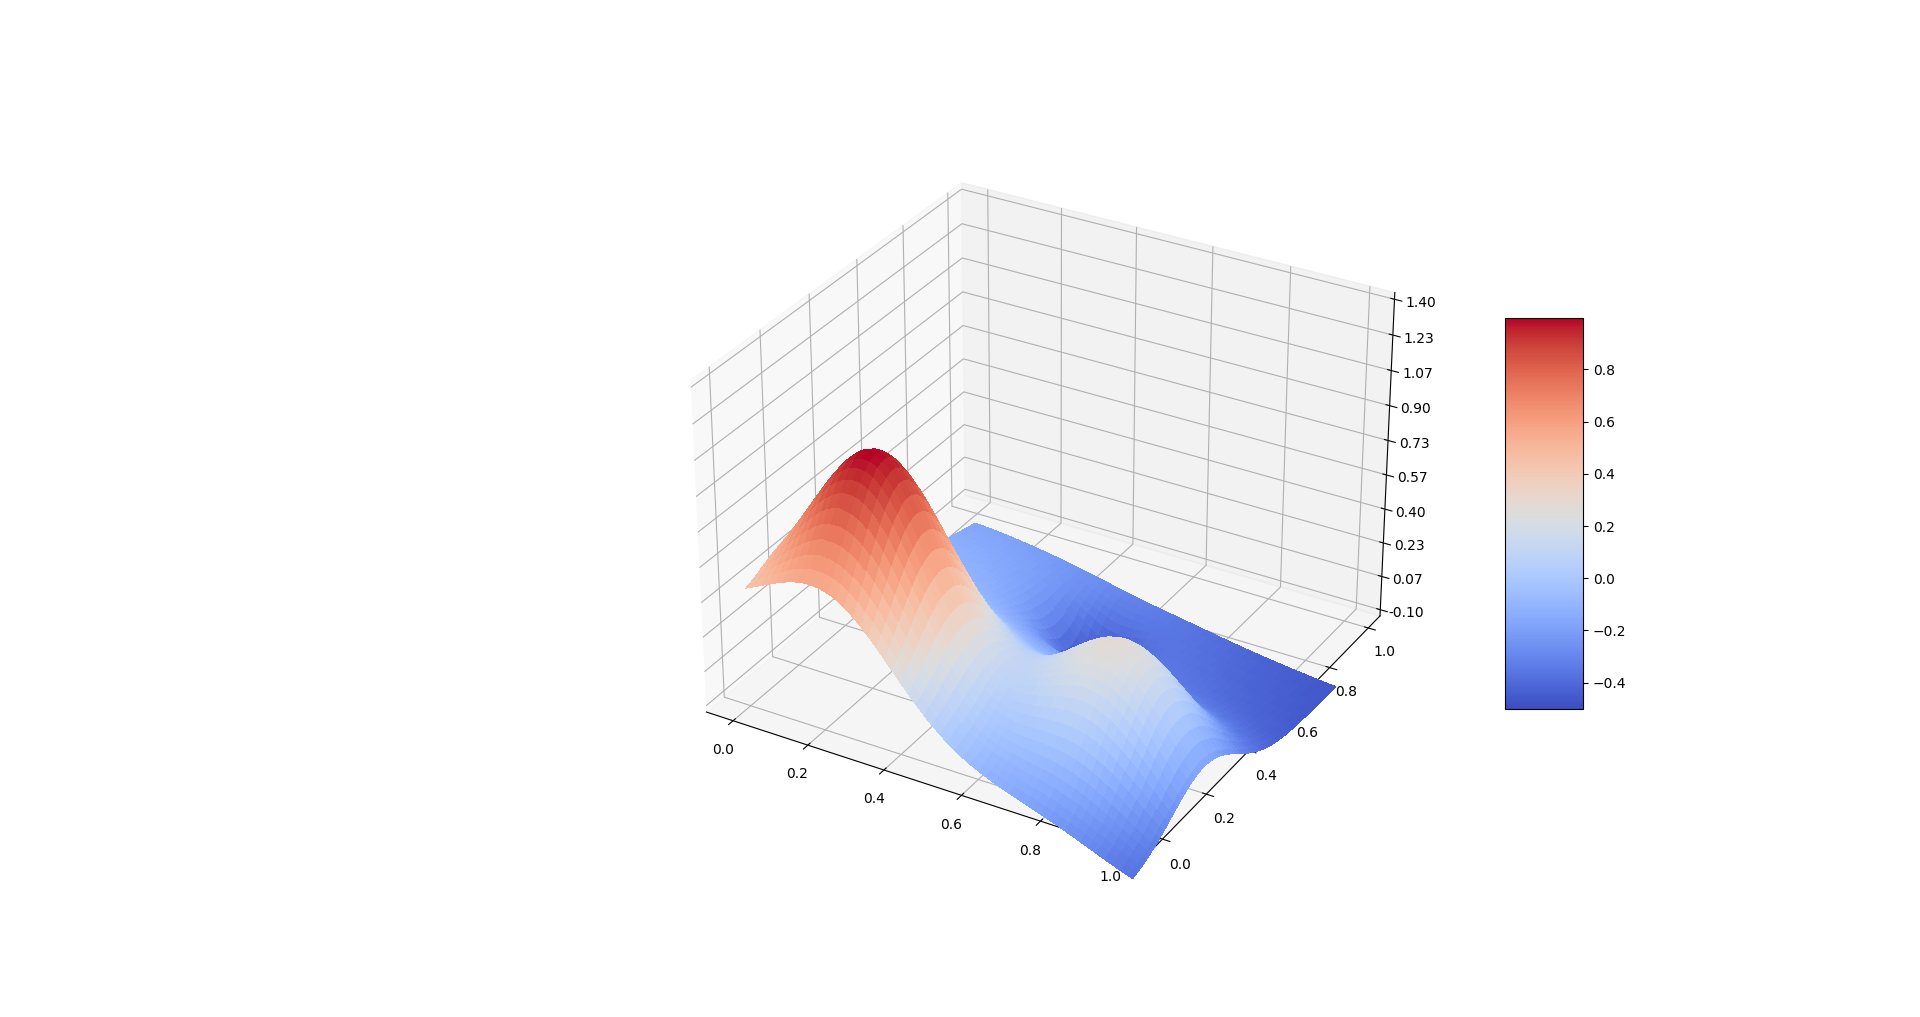
\includegraphics[width = 1\linewidth]{C:/Users/Sander/Documents/GitHub/FYS-STK4155/Project2/Project2/Report/Figures/FrankOG.PNG}
\caption{\label{fig:Franke} A plot of the Franke function discretized with 100 times a 100 observations. The function is standardized and normalized such that the mean is zero and the variance is 1 and the maximum value is 1.}
\end{figure}

\begin{center}
\large{\textbf{Concepts of gradient descent and the cost function}}
\end{center}

\noindent In the last project, we utilized least squares solutions on the form $\boldsymbol{\hat{\beta}} = (\textbf{X}^T\textbf{X})^{-1}\textbf{X}^T\hat{y}$ in order to find the regression coefficients yielding the lowest residual sum of squares. However, this method relies on taking an matrix inverse of the data, which often is not feasible. Another approach which does not utilize matrix inversion is gradient descent. This method instead relies on finding the minimum value of some cost function dependent on the regression coefficients. In this exercise, we will use the MSE as the cost function is given by equation \ref{eq:MSEdef}

\begin{equation}\label{eq:MSEdef}
\begin{aligned}
MSE = C(\boldsymbol{\beta}) = \frac{1}{n}\sum_{i = 1}^n (f - \hat{y})^2
\end{aligned}
\end{equation}

\noindent where f is the Franke function we are trying to predict and $\hat{y}$ is the prediction. Like previously mentioned, we want to find where this function has its minimum, as this point will yield the best regression coefficients. Gradient descent does not attempt to find this point directly, but iteratively. We can find the gradient of equation \ref{eq:MSEdef} and iteratively move the values of our regression coefficients along the line of most negative gradient. After a given number of iterations, we are bound to find the minimum of the cost function, or at least a local minimum (this will be discussed later). In order to find the gradient, we can simply take the partial derivative of equation \ref{eq:MSEdef} with respect to each individual regression coefficient

\begin{equation}\label{eq:MSEder}
\begin{aligned}
\frac{\partial C(\boldsymbol{\beta})}{\partial \boldsymbol{\beta}} 
\\
\frac{\partial \frac{1}{n} \sum_{i = 1}^n (f-\hat{y})^2}{\partial \boldsymbol{\beta}} 
\\
\frac{\partial \frac{1}{n} \sum_{i = 1}^n (f-\textbf{X}\boldsymbol{\hat{\beta}})^2}{\partial \boldsymbol{\beta}} 
\\
\frac{2}{n} \sum_{i = 1}^n \textbf{X}(f - \textbf{X}\boldsymbol{\hat{\beta}}) 
\end{aligned}
\end{equation}

\noindent As mentioned, we iteratively follow the direction in which the gradient is most negative. The number of iterations to perform is called the epoch and is usually just set to a very high number. When we are approaching the minimum or a local minimum, the algorithm which only follows the gradient will be "stuck" and wiggle back and fourth around this minimum or local minimum. Therefore, any iterations following the point of becoming "stuck" is useless, so the algorithm should be stopped at this point.
\\
We have so far only discussed in which direction we are to move, but how large steps should we take in that direction? This parameter is called the learning rate and is typically in the between zero and one (around $0.01$). The learning parameter can either be static or adaptive. The former means that we are only moving a set distance every iteration, while the latter means that we are changing the distance we are moving depending on what iterations we are currently on. A adaptive learning rate depends on the schedule which sets the learning rate for each epoch iteration. In this project we use the time based schedule which is given by equation \ref{eq:scheduleTIME}

\begin{equation}\label{eq:scheduleTIME}
\begin{aligned}
\frac{t_0}{t + t_1}
\end{aligned}
\end{equation}

\noindent where $t_0$ and $t_1$ are constants and t is given by epoch iterations $\times$ number of samples. 
\\
The problem with gradient descent is that if we have a very large number of features (polynomial degrees here), the gradient descent algorithm will take a very long time to run. To counter this problem, we introduce a variant of the gradient descent called stochastic gradient descent.

\begin{center}
\large{\textbf{Taking a stochastic approach to gradient descent}}
\end{center}

\noindent The stochastic gradient descent approach relies on simply utilizing a part of the entire data. The part used is called batch or mini-batch and can be just a single observation (actual stochastic gradient descent) or some where in between one and the number of observations (semi-stochastic gradient descent). This technique works as we are iterating over the number of batches as well as the number of epochs, each time taking a random sample from the original observations. Taking only a sample from the observation works because we are repeating the gradient descent process a large number of times equal to $\frac{\textrm{number of observations}}{\textrm{size of batch}}$. Since we are only utilizing one or a few number of observations, equation \ref{eq:MSEder} can be written as

\begin{equation}\label{eq:MSEderSTO}
\begin{aligned}
2 \textbf{X}(f - \textbf{X}\boldsymbol{\hat{\beta}}) 
\end{aligned}
\end{equation}

\noindent and the t in equation \ref{eq:scheduleTIME} will instead be epoch iteration $\times$ number of samples $+$ batch iteration.
\\
So far we have only considered the gradient descent in terms of its least squares equivalent, however, we also want to implement the ridge equivalent. In the Ridge case, the gradient descent concept and algorithm is exactly the same as the OLS case, but the gradient at which we try to find the MSE minimum look slightly different as we need to add a penalty term $\lambda \times \boldsymbol{\hat{\beta}}$ as shown in equation \ref{eq:MSEderSTOridge}

\begin{equation}\label{eq:MSEderSTOridge}
\begin{aligned}
2 \textbf{X}(f - \textbf{X}\boldsymbol{\hat{\beta}}) + \lambda \boldsymbol{\hat{\beta}}
\end{aligned}
\end{equation}

\noindent where the penalty parameter $\lambda$ is typically between zero and one. 

\begin{center}
\large{\textbf{Parameter dependencies for static learning rate}}
\end{center}

\noindent So far we have merely discussed the theoretical concepts of gradient descent, but now we will implement to perform the stochastic gradient descent. We will then vary the different parameters and see how our cost function varies with the different parameters. First, let us set up some standard parameters so we keep the analysis consistent as seen in table \ref{tab:standardParam}

\begin{table}[h]
\caption{\label{tab:standardParam} An overview of standard parameters to be used in the analysis.}
\centering
\begin{tabular}{c|c|c|c|c}
 & static OLS & static Ridge & adaptive OLS & adaptive Ridge\\
\hline
Number of observation n & $100$ & $100$ & $100$ & $100$\\
\hline
Noise-level & $0.001$ & $0.001$ & $0.001$ & $0.001$\\
\hline
Penalty $\lambda$ & None & $0.01$ & None & $0.01$\\
\hline
Model complexity p & $5$ & $5$ & $5$ & $5$\\
\hline
Batch size & $10$ & $10$ & $10$ & $10$\\
\hline
Epoch size & $100$ & $100$ & $100$ & $100$\\
\hline
Initial learning rate & $0.01$ & $0.01$ & $0.01$ & $0.01$\\
\hline
Schedule & None & None & $\frac{t_0}{t+t_1}$ & $\frac{t_0}{t+t_1}$\\
\end{tabular}
\end{table}

\noindent We can now use the values in table \ref{tab:standardParam} as a standard when we want to study the dependence on a single parameter. Let us first study how the MSE varies as function of an increasing number of epoch iterations using our standard parameters with static learning rate

\begin{figure}[H]
\centering
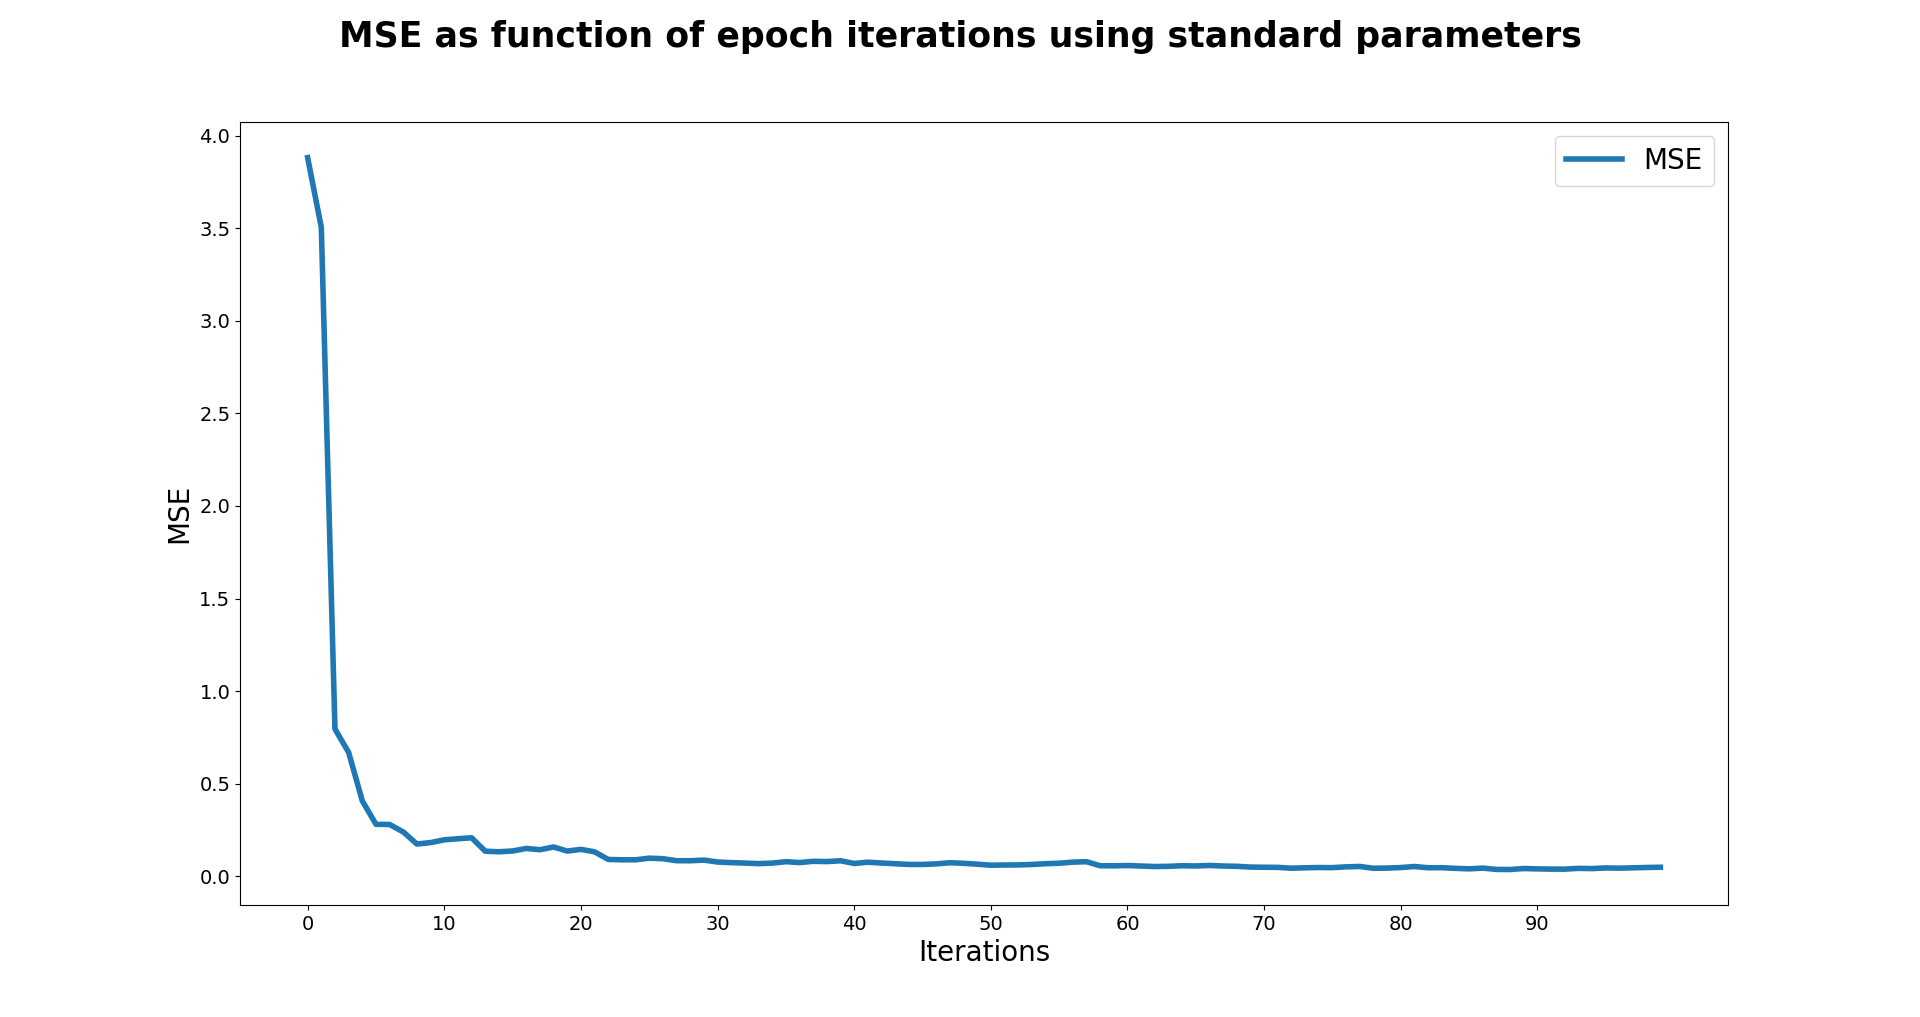
\includegraphics[width = 1\linewidth]{C:/Users/Sander/Documents/GitHub/FYS-STK4155/Project2/Project2/Report/Figures/MSEvsEPOCH_StandardOLS.PNG}
\caption{\label{fig:MSEvsEPOCHstandard} The MSE as function of number of epoch iterations using static learning rate and OLS equivalent SGD.}
\end{figure}

\begin{figure}[H]
\centering
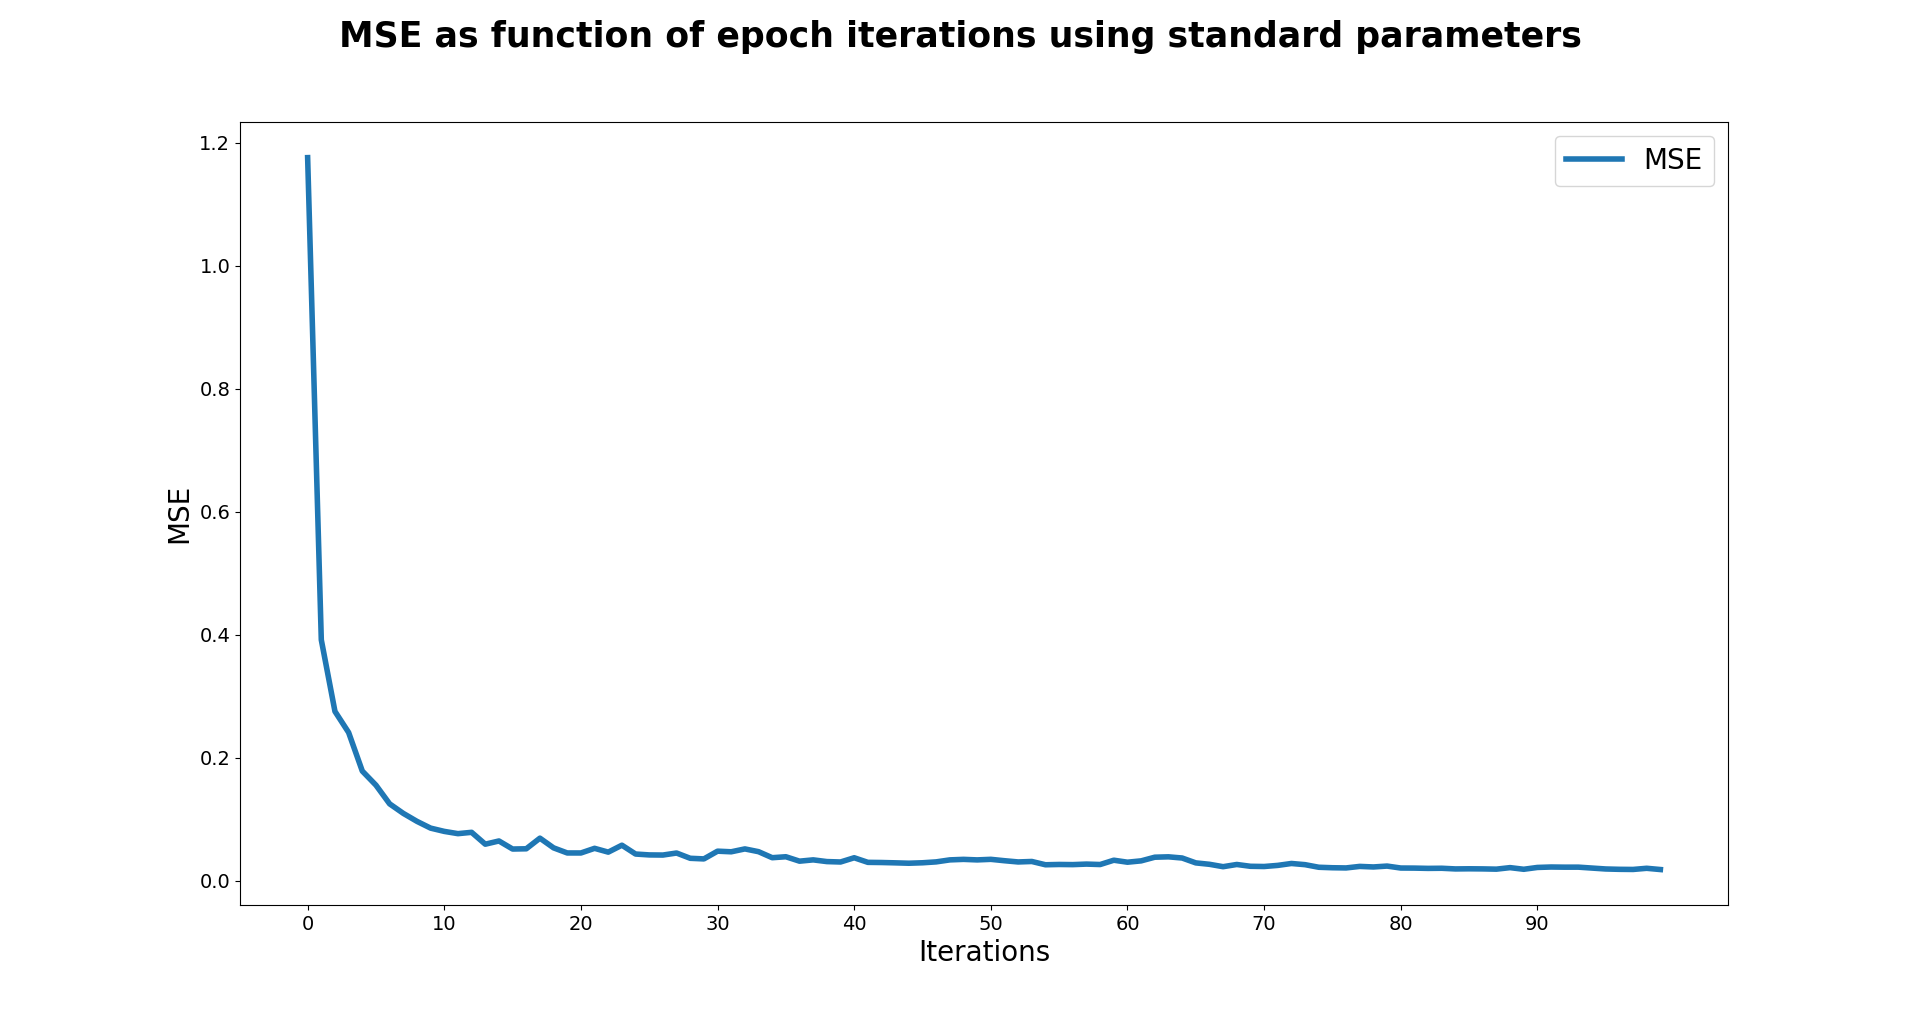
\includegraphics[width = 1\linewidth]{C:/Users/Sander/Documents/GitHub/FYS-STK4155/Project2/Project2/Report/Figures/MSEvsEPOCH_StandardRIDGE.PNG}
\caption{\label{fig:MSEvsEPOCHstandardRidge} The MSE as function of number of epoch iterations using static learning rate and Ridge equivalent SGD.}
\end{figure}

\noindent Figures \ref{fig:MSEvsEPOCHstandard} and \ref{fig:MSEvsEPOCHstandardRidge} shows that the MSE drastically increases as function of the number of epoch iterations, particularly at low number of iterations. At higher number of iterations, say around 30, the MSE keeps decreasing, but at a lower rate. One can also observe that the Ridge SGD starts at a lower MSE than the OLS SGD which indicate that Ridge algorithms fits the data better. Let us now see how the MSE changes as function of both epoch iterations and the size of the batch. We will then use the standard parameters, but change the batch size in the span $[100, 10, 1]$ and the results are shown in figures \ref{fig:MSEvsEPOCHbatchOLS} and \ref{fig:MSEvsEPOCHbatchRIDGE}

\begin{figure}[H]
\centering
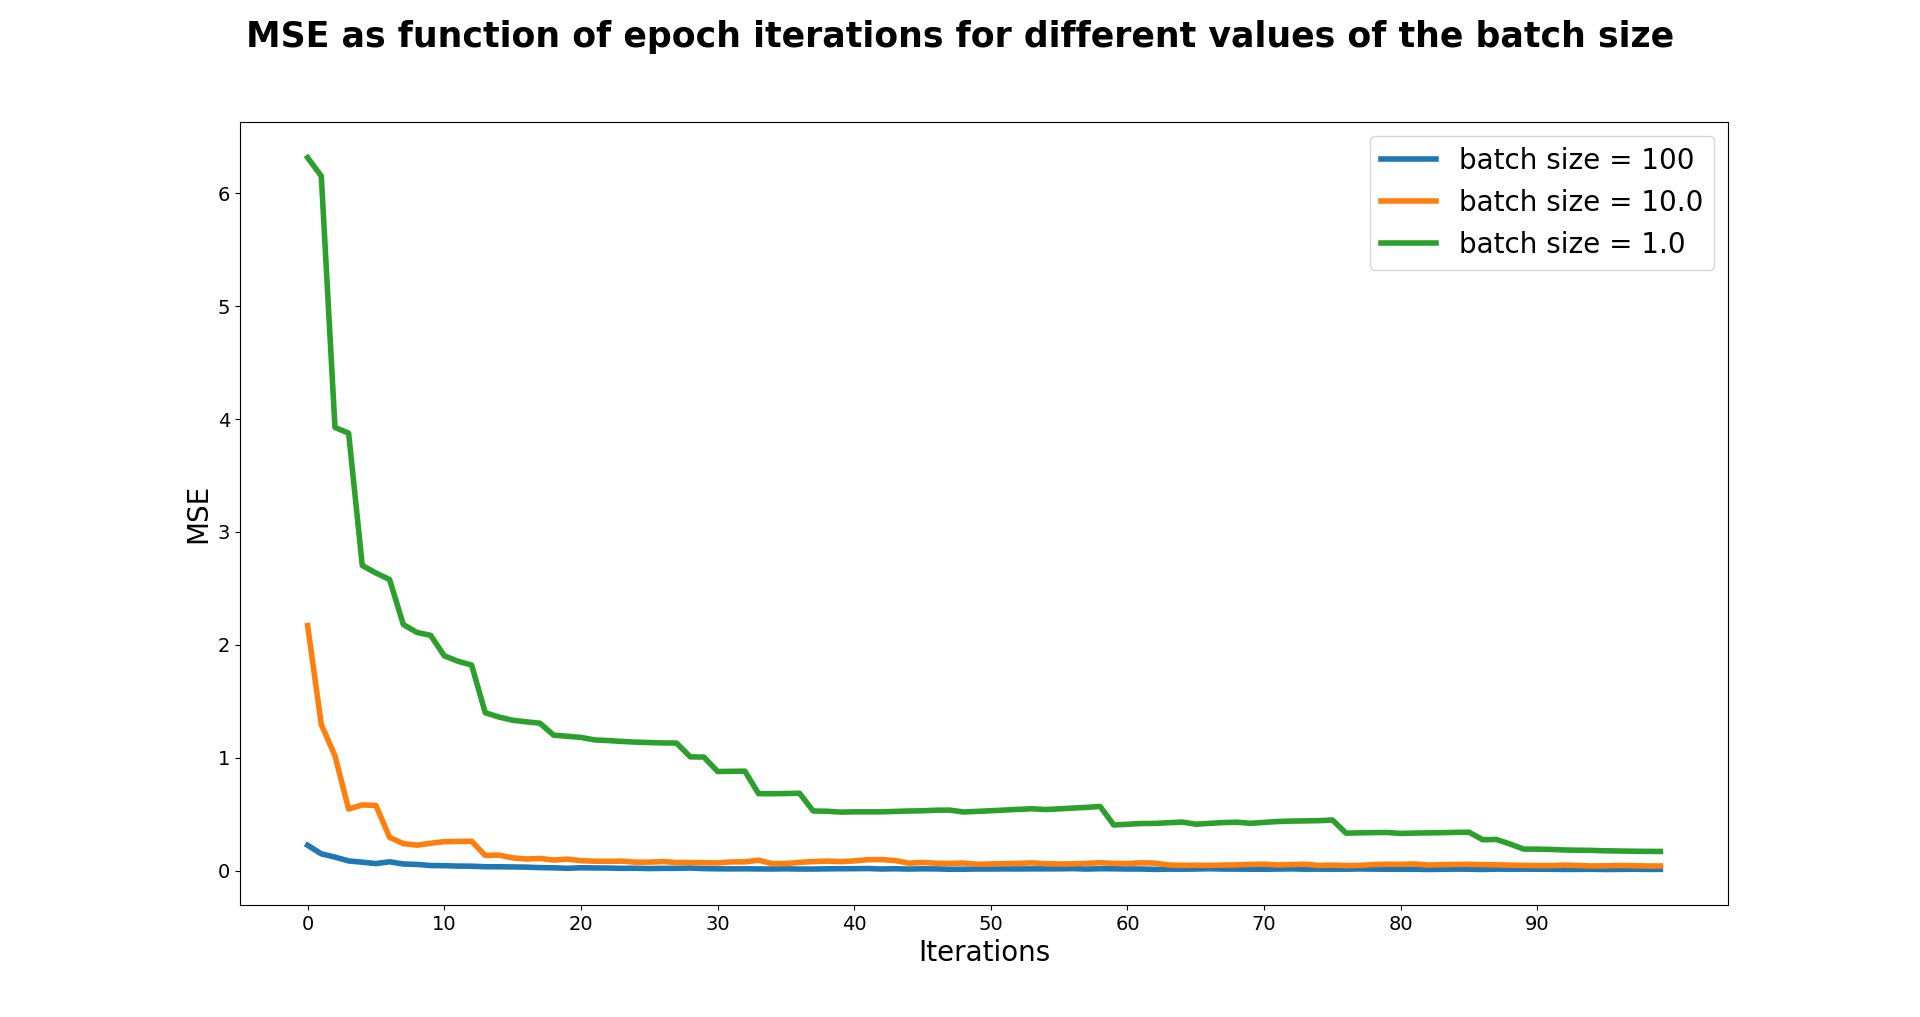
\includegraphics[width = 1\linewidth]{C:/Users/Sander/Documents/GitHub/FYS-STK4155/Project2/Project2/Report/Figures/MSEvsEPOCH_BatchOLS.PNG}
\caption{\label{fig:MSEvsEPOCHbatchOLS} The MSE as function of number of epoch iterations and batch sizes using static learning rate and OLS equivalent SGD.}
\end{figure}

\begin{figure}[H]
\centering
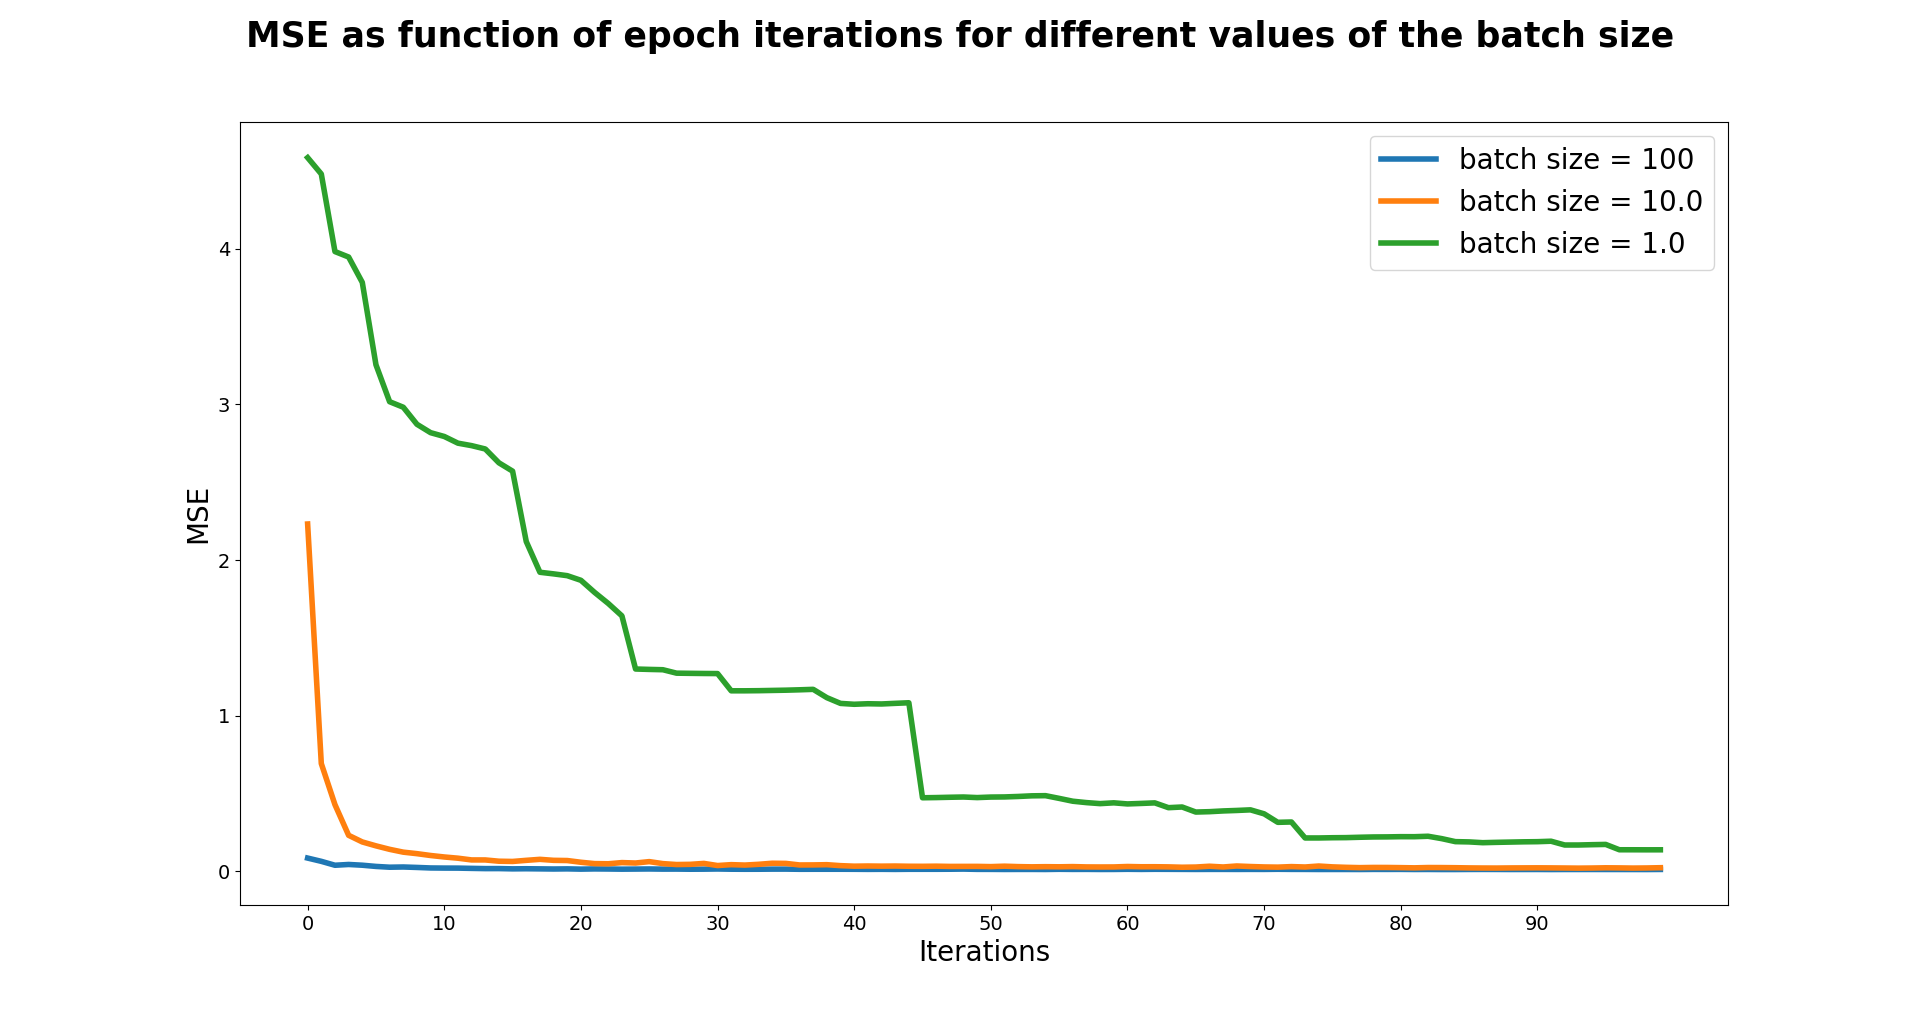
\includegraphics[width = 1\linewidth]{C:/Users/Sander/Documents/GitHub/FYS-STK4155/Project2/Project2/Report/Figures/MSEvsEPOCH_BatchRIDGE.PNG}
\caption{\label{fig:MSEvsEPOCHbatchRIDGE} The MSE as function of number of epoch iterations and batch sizes using static learning rate and Ridge equivalent SGD.}
\end{figure}

\noindent It can be observed from figures \ref{fig:MSEvsEPOCHbatchOLS} and \ref{fig:MSEvsEPOCHbatchRIDGE} that increasing the batch size drastically decreases the MSE. The batch size of 100 is equivalent to gradient descent (we use all observations) and it clearly has the lowest MSE for both the OLS and Ridge SGD. However, using the entirety of the data set can be extremely costly in terms of computational power, so it is not optimal for large data sets. What we also observe is that the difference in MSE between the batch sizes decreases for higher number of epoch iterations. In other words, we can utilize smaller batch sizes as long as we have a sufficiently large epoch. 
\\
Now let us see how the MSE varies as function of learning rate. We can again plot the MSE versus epoch iterations with our standard parameters, but vary the learning rate in the span $[0.0001, 0.001, 0.01]$

\begin{figure}[H]
\centering
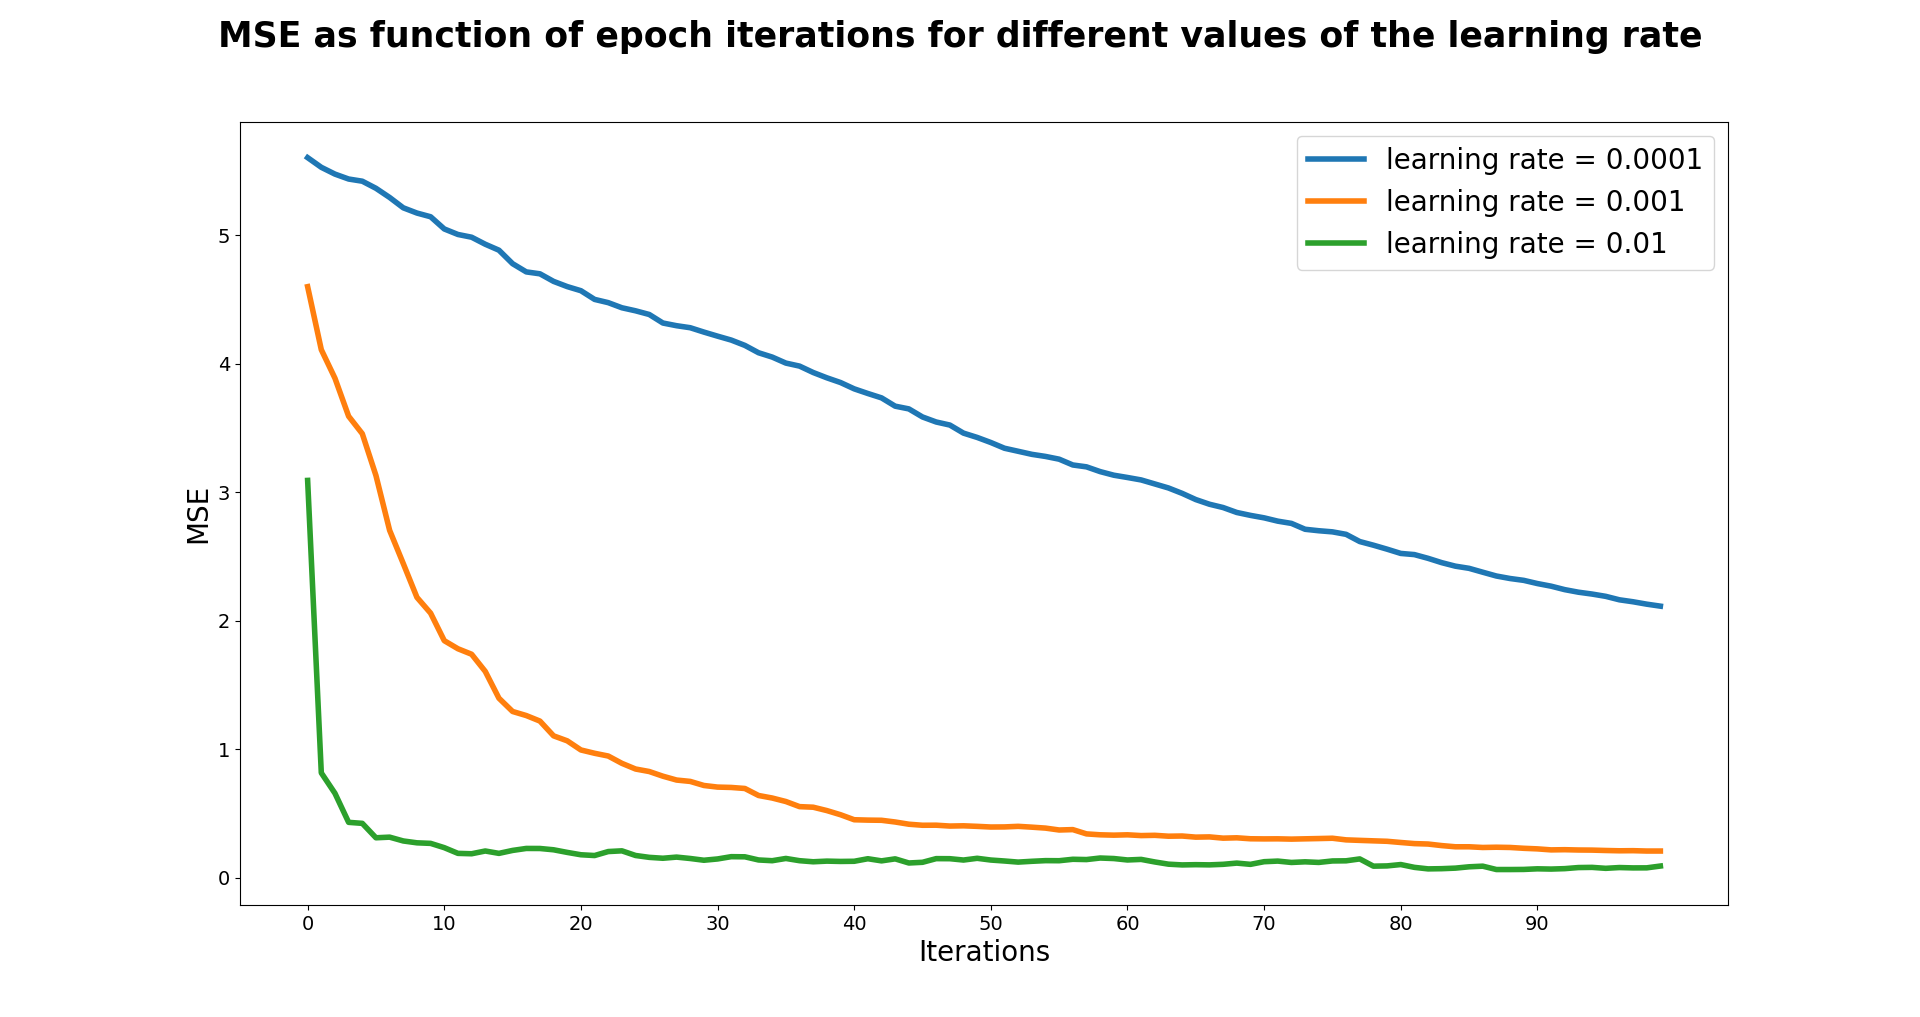
\includegraphics[width = 1\linewidth]{C:/Users/Sander/Documents/GitHub/FYS-STK4155/Project2/Project2/Report/Figures/MSEvsEPOCH_LearnOLS.PNG}
\caption{\label{fig:MSEvsEPOCHlaernOLS} The MSE as function of number of epoch iterations and learning rates using static learning rate and OLS equivalent SGD.}
\end{figure}

\begin{figure}[H]
\centering
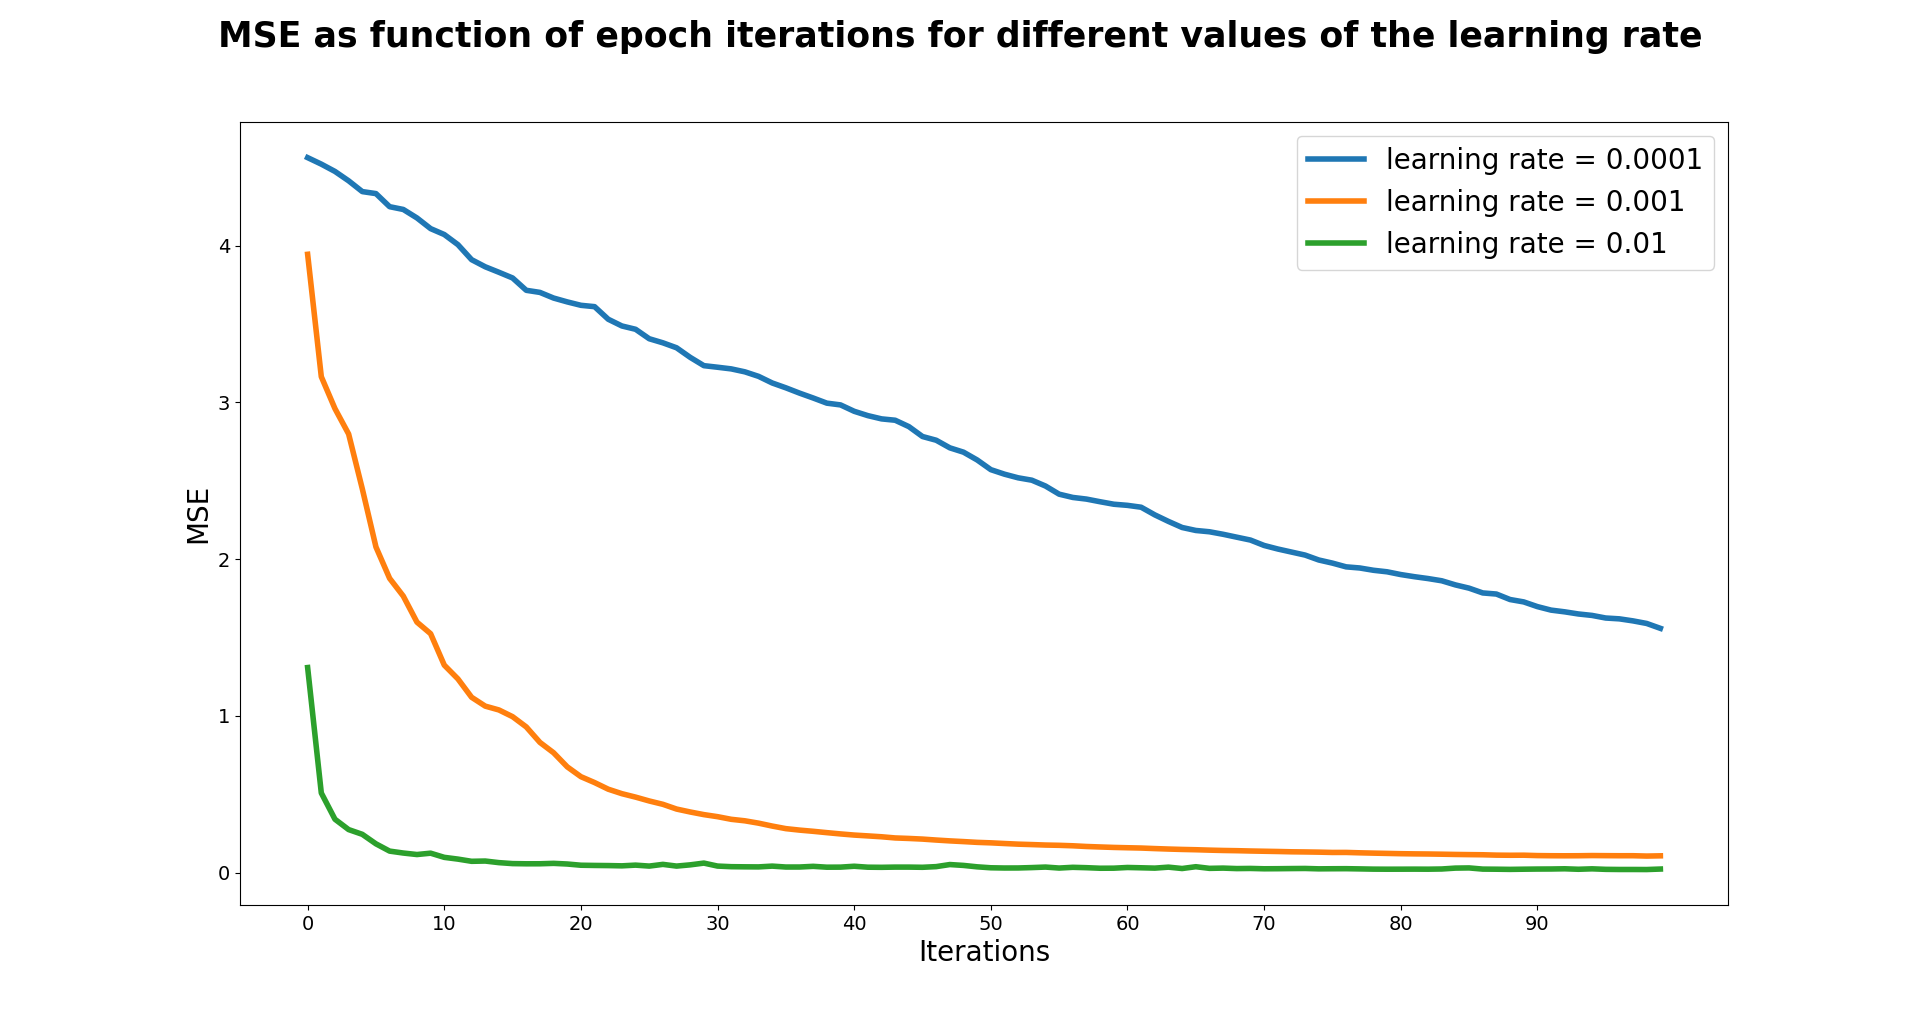
\includegraphics[width = 1\linewidth]{C:/Users/Sander/Documents/GitHub/FYS-STK4155/Project2/Project2/Report/Figures/MSEvsEPOCH_LearnRIDGE.PNG}
\caption{\label{fig:MSEvsEPOCHlearnRIDGE} The MSE as function of number of epoch iterations and learning rates using static learning rate and Ridge equivalent SGD.}
\end{figure}

\noindent One can observe from figures \ref{fig:MSEvsEPOCHlaernOLS} and \ref{fig:MSEvsEPOCHlearnRIDGE} that increasing the learning rate decreases the MSE for a low number of epoch iterations. However, the MSE of learning rates $0.01$ and $0.001$ converge for a higher number of epoch iterations. The MSE of the learning rate $0.0001$ does not drop exponentially, but linearly. This may be due to the learning rate is so small that the SGD takes a very long time to reach any kind of minimum, making the process too slow for the number of epoch iterations shown here. What we observe overall is that a learning rate anywhere over $0.001$ is fine as long as we have sufficiently many epoch iterations. 
\\
We can also study the how the MSE of the Ridge SGD changes as function of the number of epoch iterations and the penalty parameter $\lambda$. We again use the standard parameters but change the penalty parameter in the span $[0.0001, 0.001, 0.01, 0.1, 1]$ and the results are shown in figure \ref{fig:MSEvsEPOCHlambRIDGE}

\begin{figure}[H]
\centering
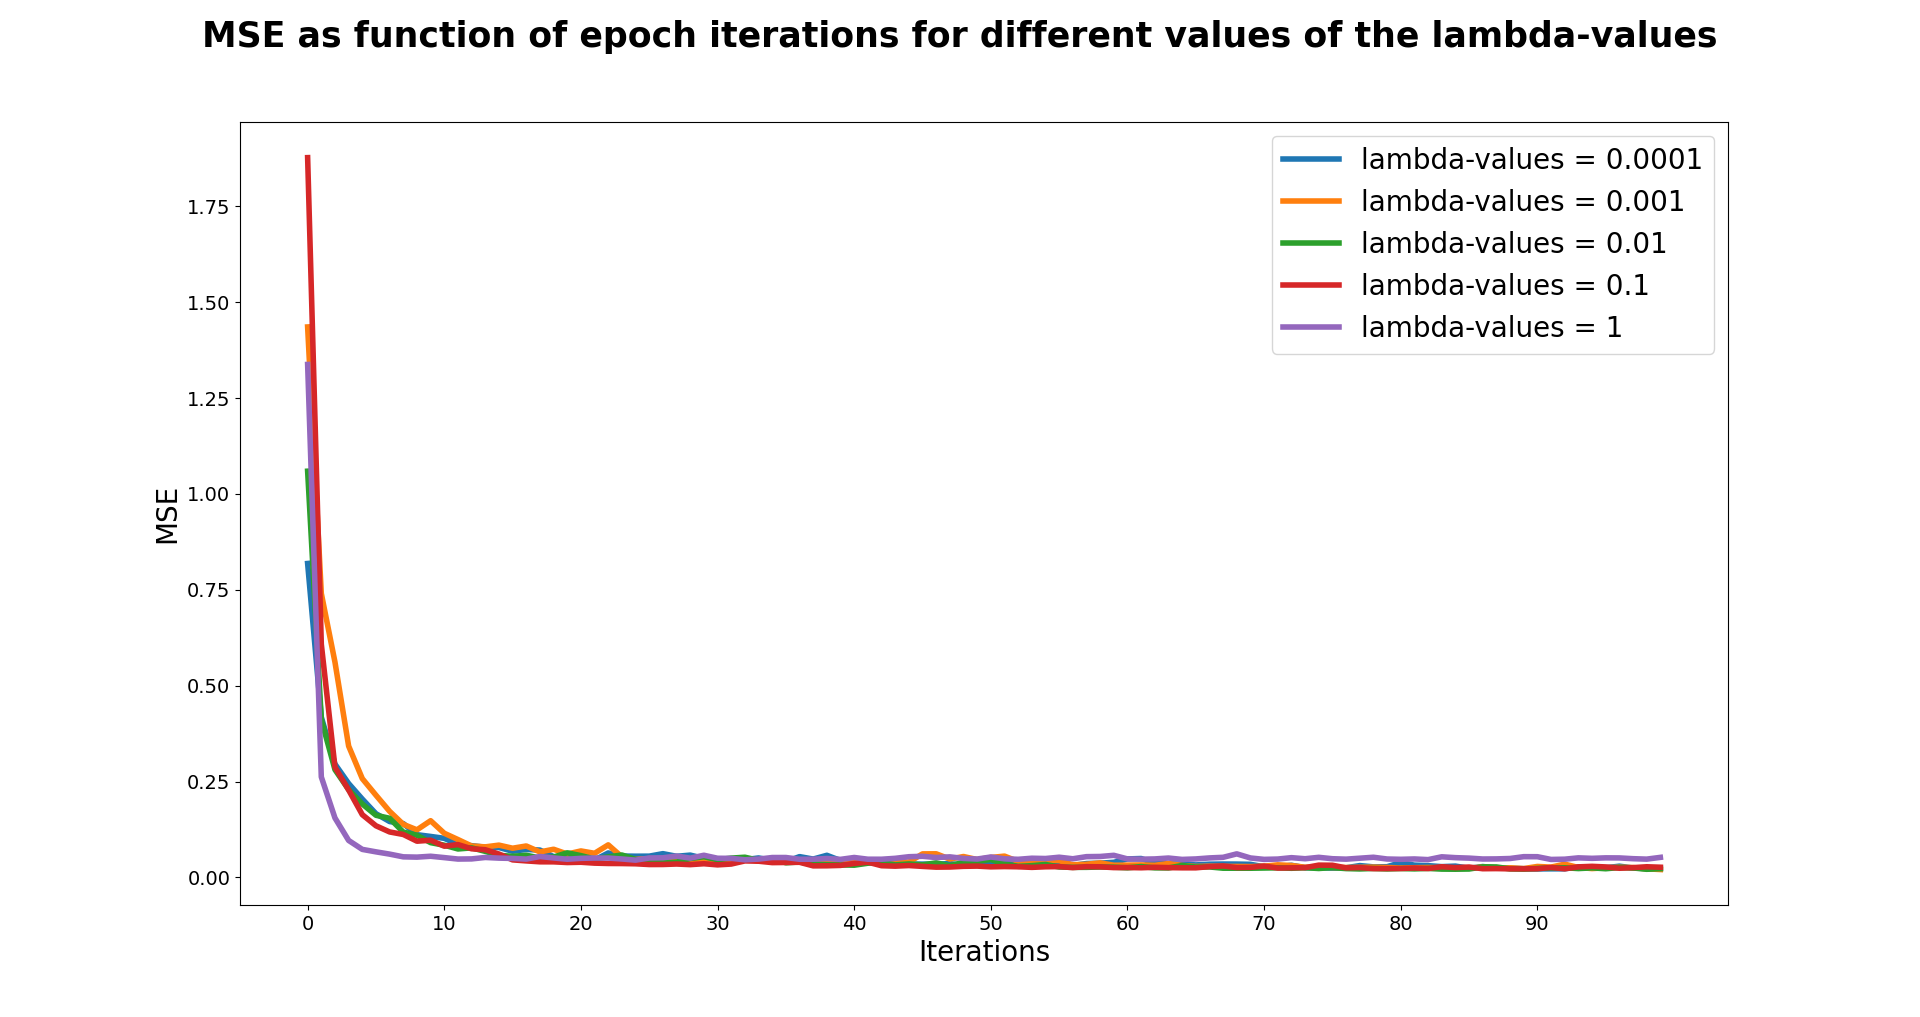
\includegraphics[width = 1\linewidth]{C:/Users/Sander/Documents/GitHub/FYS-STK4155/Project2/Project2/Report/Figures/MSEvsEPOCH_lambRIDGE.PNG}
\caption{\label{fig:MSEvsEPOCHlambRIDGE} The MSE as function of number of epoch iterations and penalty parameter $\lambda$ using static learning rate and Ridge equivalent SGD.}
\end{figure}

\noindent One can observe from figure \ref{fig:MSEvsEPOCHlambRIDGE} that the different penalty parameters yields similar results. One interesting observations is that the penalty parameter of $1$ yields the lowest MSE for a low number of epoch iterations, while it yields the highest MSE for a high number of epoch iterations. This may be caused by the fact that some of the regression coefficients are set close to zero and therefore do not contribute much to the overall cost function. It may be that the minimum of this reduced cost function has a minimum or local minimum with higher MSE than that of the less reduced cost function.

\begin{center}
\large{\textbf{Parameter dependencies for scheduled learning rate}}
\end{center}

\noindent We now aim to repeat the above analysis, but with a scheduled/adaptive learning rate. The learning rate will change as according to $\frac{t_0}{t+t_1}$ where $t_0 = 5$, $t_1 = 50$ and where t is constantly changing as function of epoch and batch iterations such that $t = $ current epoch iteration $\times$ batch size $+$ current batch iteration. The hopes for the scheduled learning rate is that we take large steps when we are far from the minimum of the cost function, while we take smaller steps as we approach said minimum. This will decrease our chances of getting "stuck" in some local minimum as our steps are too large for us to find ourselves in such a local minimum. We can implement this schedule in the SGD algorithm and see how the MSE changes for different epoch iterations and varying parameters. We start by simply plotting the MSE as function of epoch iteration using the standard parameters of table \ref{tab:standardParam}

\begin{figure}[H]
\centering
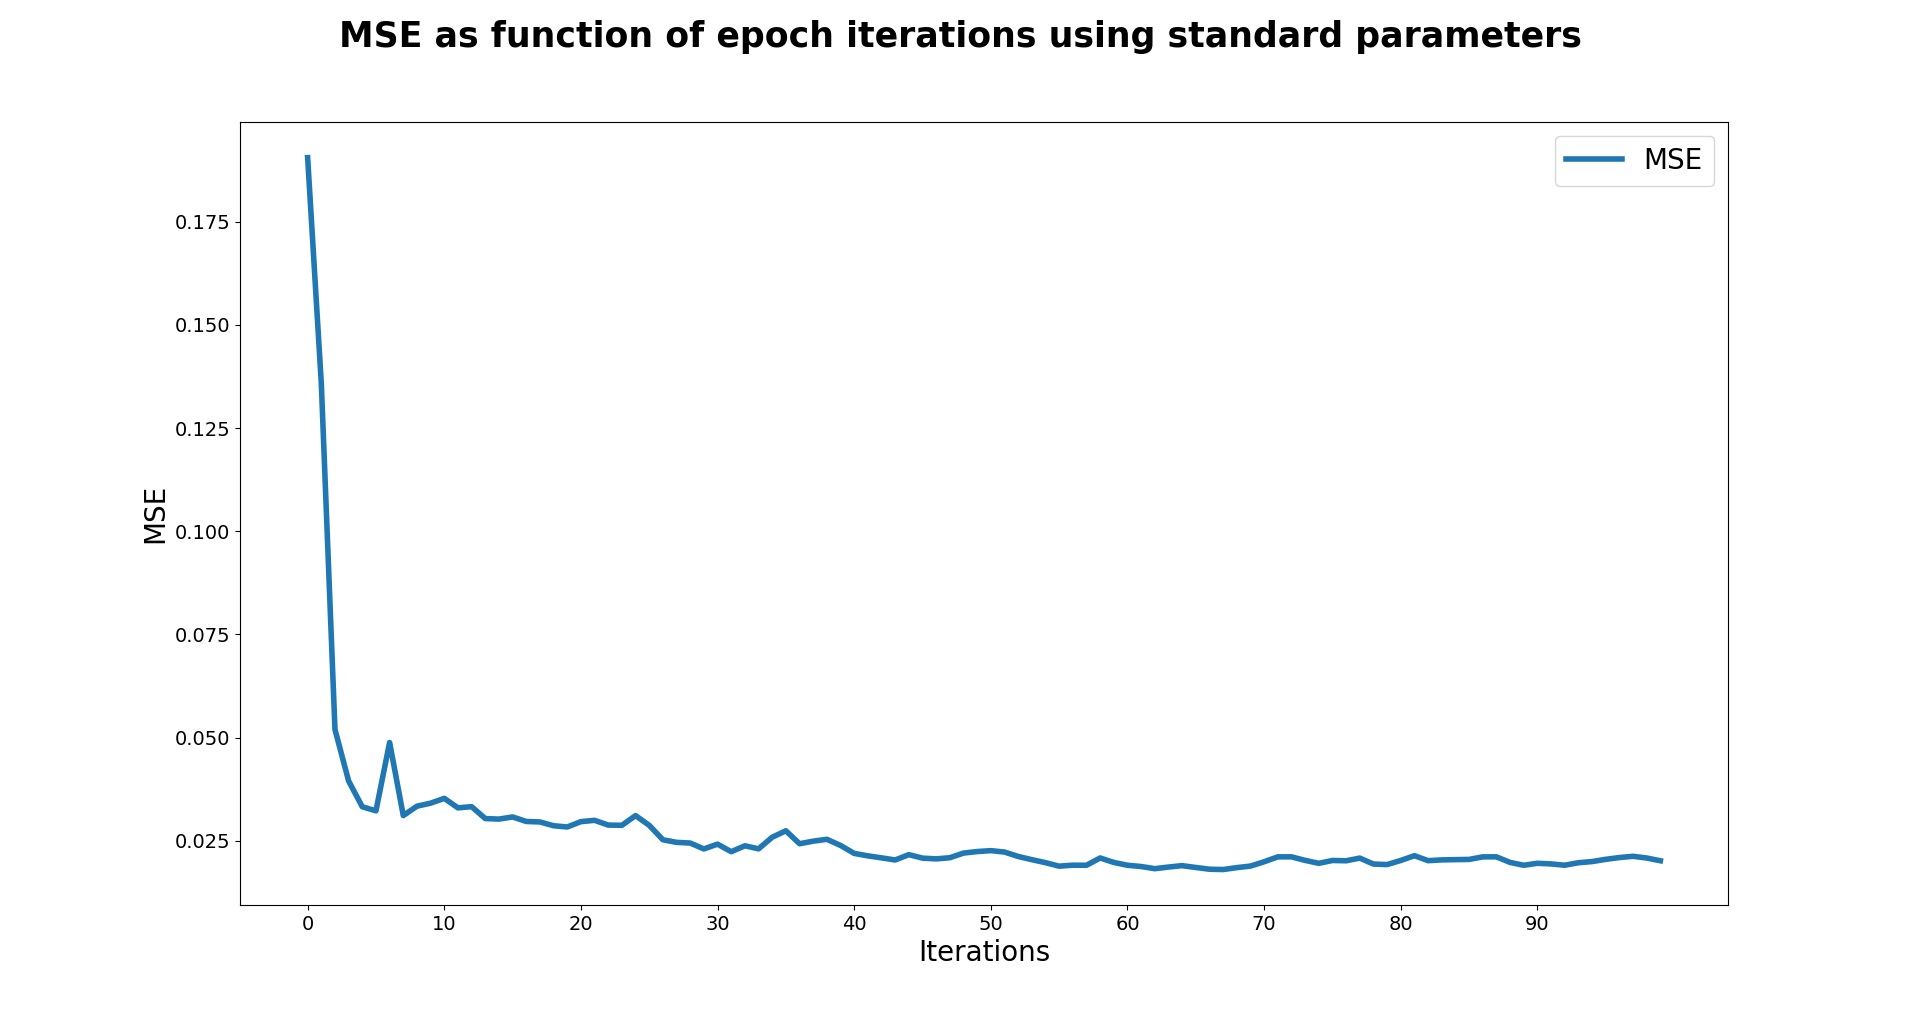
\includegraphics[width = 1\linewidth]{C:/Users/Sander/Documents/GitHub/FYS-STK4155/Project2/Project2/Report/Figures/MSEvsEPOCH_StandardOLS_schedule.PNG}
\caption{\label{fig:MSEvsEPOCHstandard_sch} The MSE as function of number of epoch iterations using a learning schedule rate and OLS equivalent SGD.}
\end{figure}

\begin{figure}[H]
\centering
\includegraphics[width = 1\linewidth]{C:/Users/Sander/Documents/GitHub/FYS-STK4155/Project2/Project2/Report/Figures/MSEvsEPOCH_StandardRIDGE_schedule.PNG}
\caption{\label{fig:MSEvsEPOCHstandardRidge_sch} The MSE as function of number of epoch iterations using a learning schedule rate and Ridge equivalent SGD.}
\end{figure}

\noindent It can be observed when comparing figures \ref{fig:MSEvsEPOCHstandard} and \ref{fig:MSEvsEPOCHstandardRidge} to figures \ref{fig:MSEvsEPOCHstandard_sch} and \ref{fig:MSEvsEPOCHstandardRidge_sch} that the MSE drops much quicker when we utilize a learning schedule. This is a direct consequence of taking larger steps when we are far away from the minimum. This ultimately leads to fewer steps to get to the minimum of the cost function. 
\\
We can also study how the MSE changes as function of batch size when we utilize a learning schedule and the result is plotted in figures QQQ and QQQ

\begin{figure}[H]
\centering
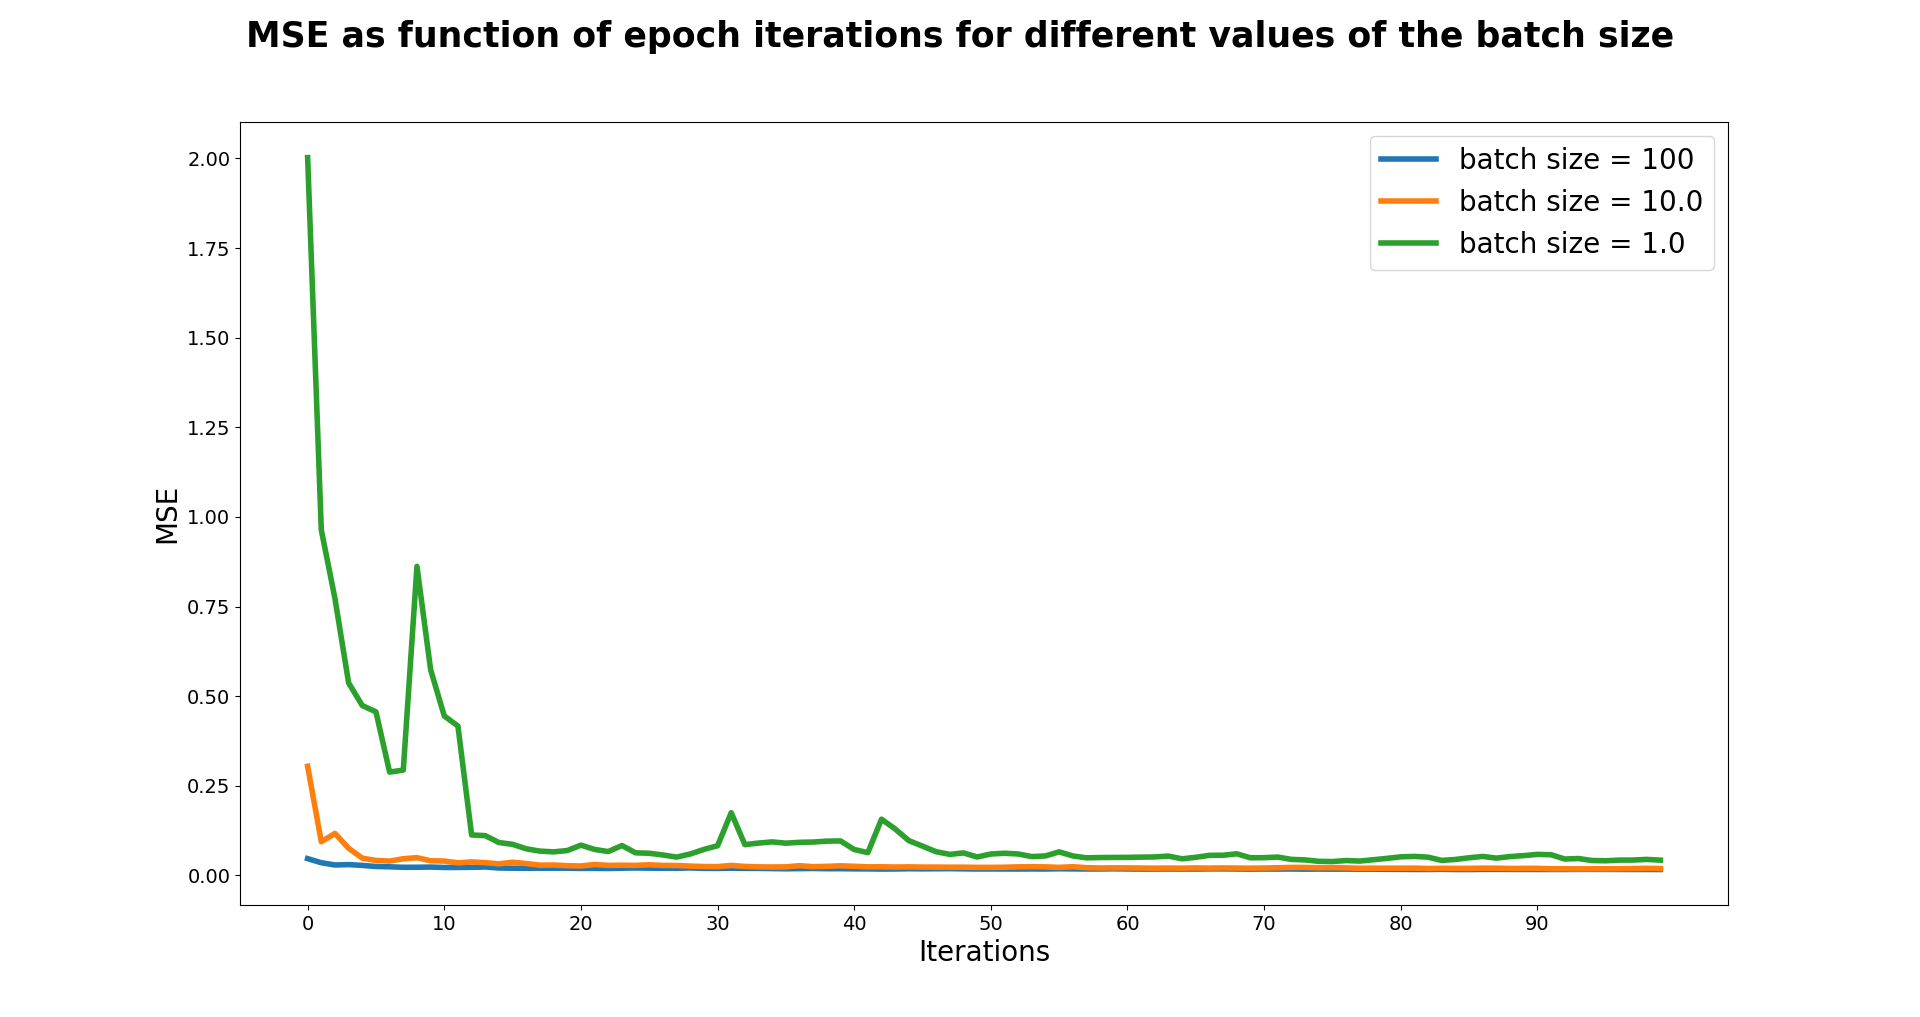
\includegraphics[width = 1\linewidth]{C:/Users/Sander/Documents/GitHub/FYS-STK4155/Project2/Project2/Report/Figures/MSEvsEPOCH_BatchOLS_schedule.PNG}
\caption{\label{fig:MSEvsEPOCHbatchOLS_sch} The MSE as function of number of epoch iterations and batch sizes using a learning schedule and OLS equivalent SGD.}
\end{figure}

\begin{figure}[H]
\centering
\includegraphics[width = 1\linewidth]{C:/Users/Sander/Documents/GitHub/FYS-STK4155/Project2/Project2/Report/Figures/MSEvsEPOCH_BatchRIDGE_schedule.PNG}
\caption{\label{fig:MSEvsEPOCHbatchRIDGE_sch} The MSE as function of number of epoch iterations and batch sizes using a learning schedule and Ridge equivalent SGD.}
\end{figure}

\noindent When we compare figures \ref{fig:MSEvsEPOCHbatchOLS} and \ref{fig:MSEvsEPOCHbatchRIDGE} to figures \ref{fig:MSEvsEPOCHbatchOLS_sch} and \ref{fig:MSEvsEPOCHbatchRIDGE_sch} we can observe that the batch size seems to play a more important role when using a learning schedule as the gap between batchs sizes are much greater than that of static learning rate. What is also observed is that the a batch size of one observation is much more "jagged" when we utilize a learning schedule. This be caused by the schedule "jumping" in and out of local minimums of the cost function. We can look at batch size equal to one for the OLS SGD in figure \ref{fig:MSEvsEPOCHbatchOLS_sch} where the MSE initially decreases a lot to around 5 iterations, but then has a large upturn in MSE. This may be one of these local minimum the algorithm found itself in. However, it does seem that the algorithm eventually finds the absolute minimum of the entire cost function as the "jagged" parts disappear for higher epoch iterations. 
\\
This phenomena seems to be a greater problem for the OLS as the Ridge SGD is nowhere near as jagged as the OLS SGD for batch size equal to one. This may be caused by the fact that some variables are reduced to a very small value, thereby removing any local minimum in that particular dimension.
\\
We can investigate the ridge implementation further by plotting plotting the MSE versus the epoch iterations for different values of the penalty parameter $\lambda$

\begin{figure}[H]
\centering
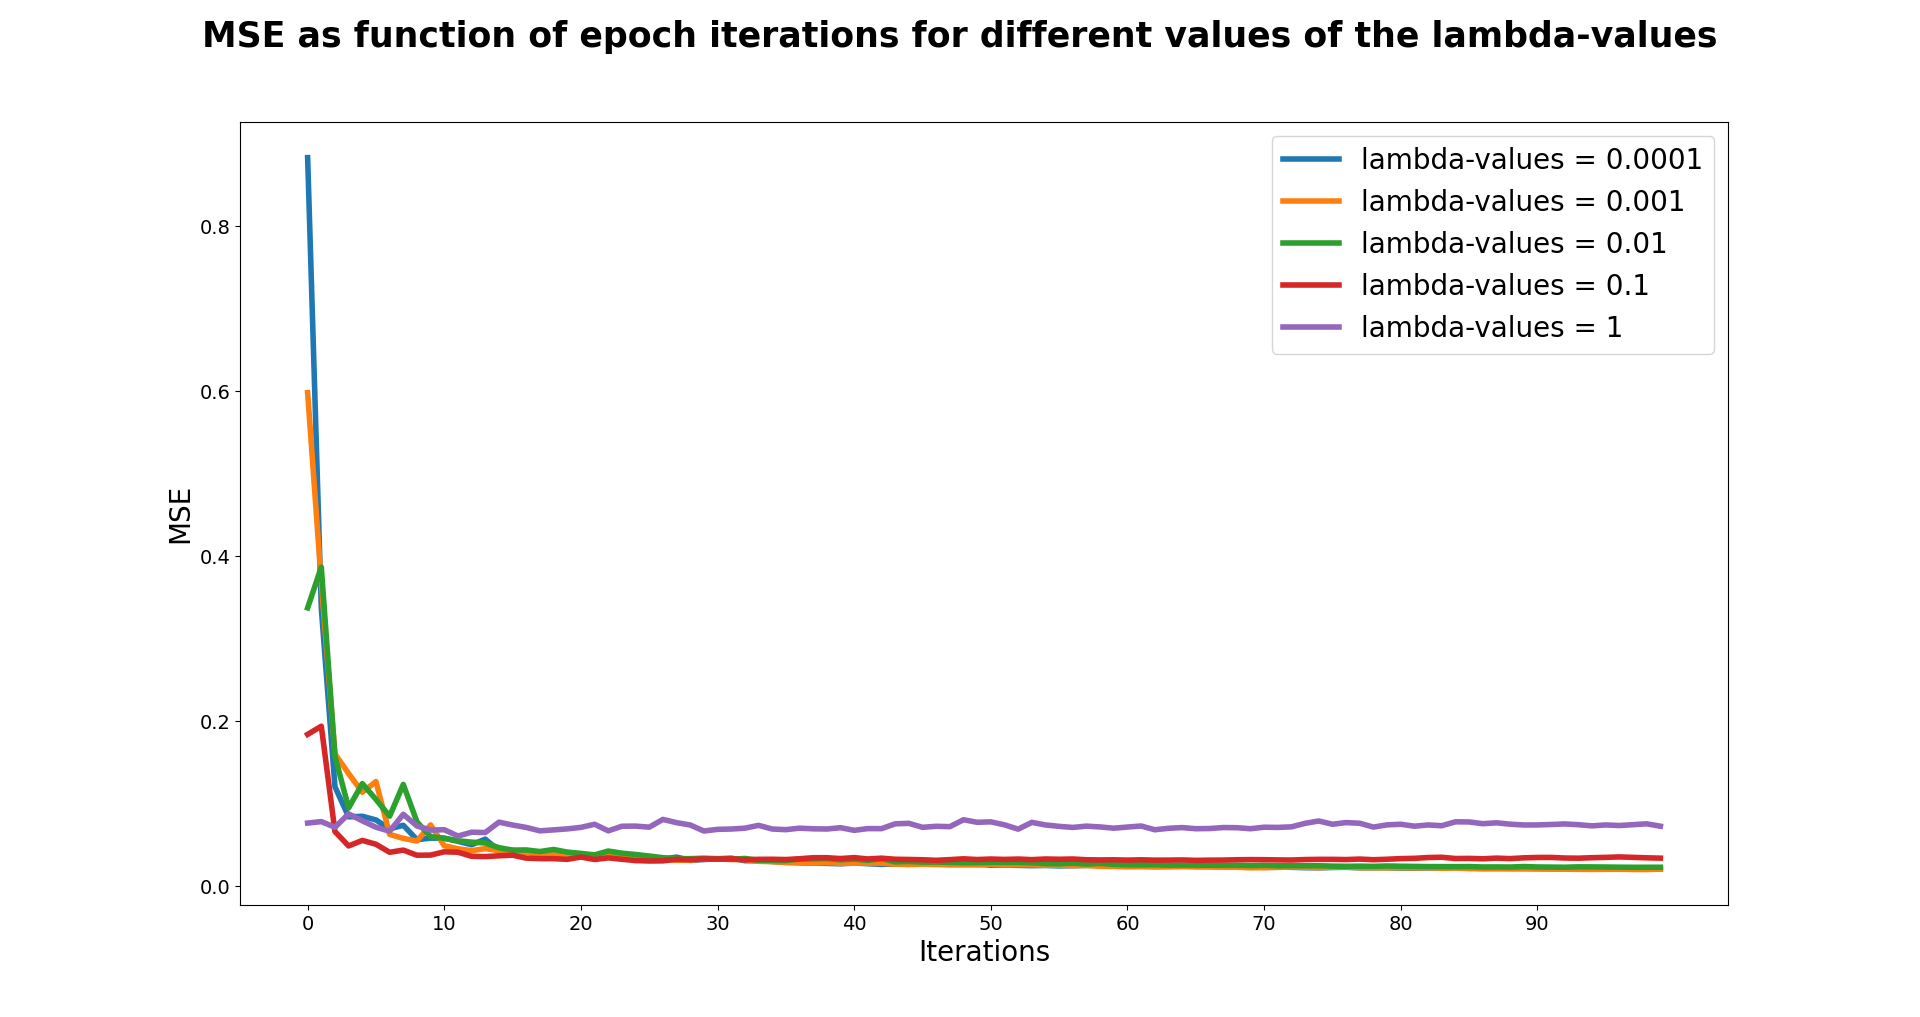
\includegraphics[width = 1\linewidth]{C:/Users/Sander/Documents/GitHub/FYS-STK4155/Project2/Project2/Report/Figures/MSEvsEPOCH_lambRIDGE_schedule.PNG}
\caption{\label{fig:MSEvsEPOCHlambRIDGE_sch} The MSE as function of number of epoch iterations and penalty parameter $\lambda$ using a learning schedule and Ridge equivalent SGD.}
\end{figure}

\begin{figure}[H]
\centering
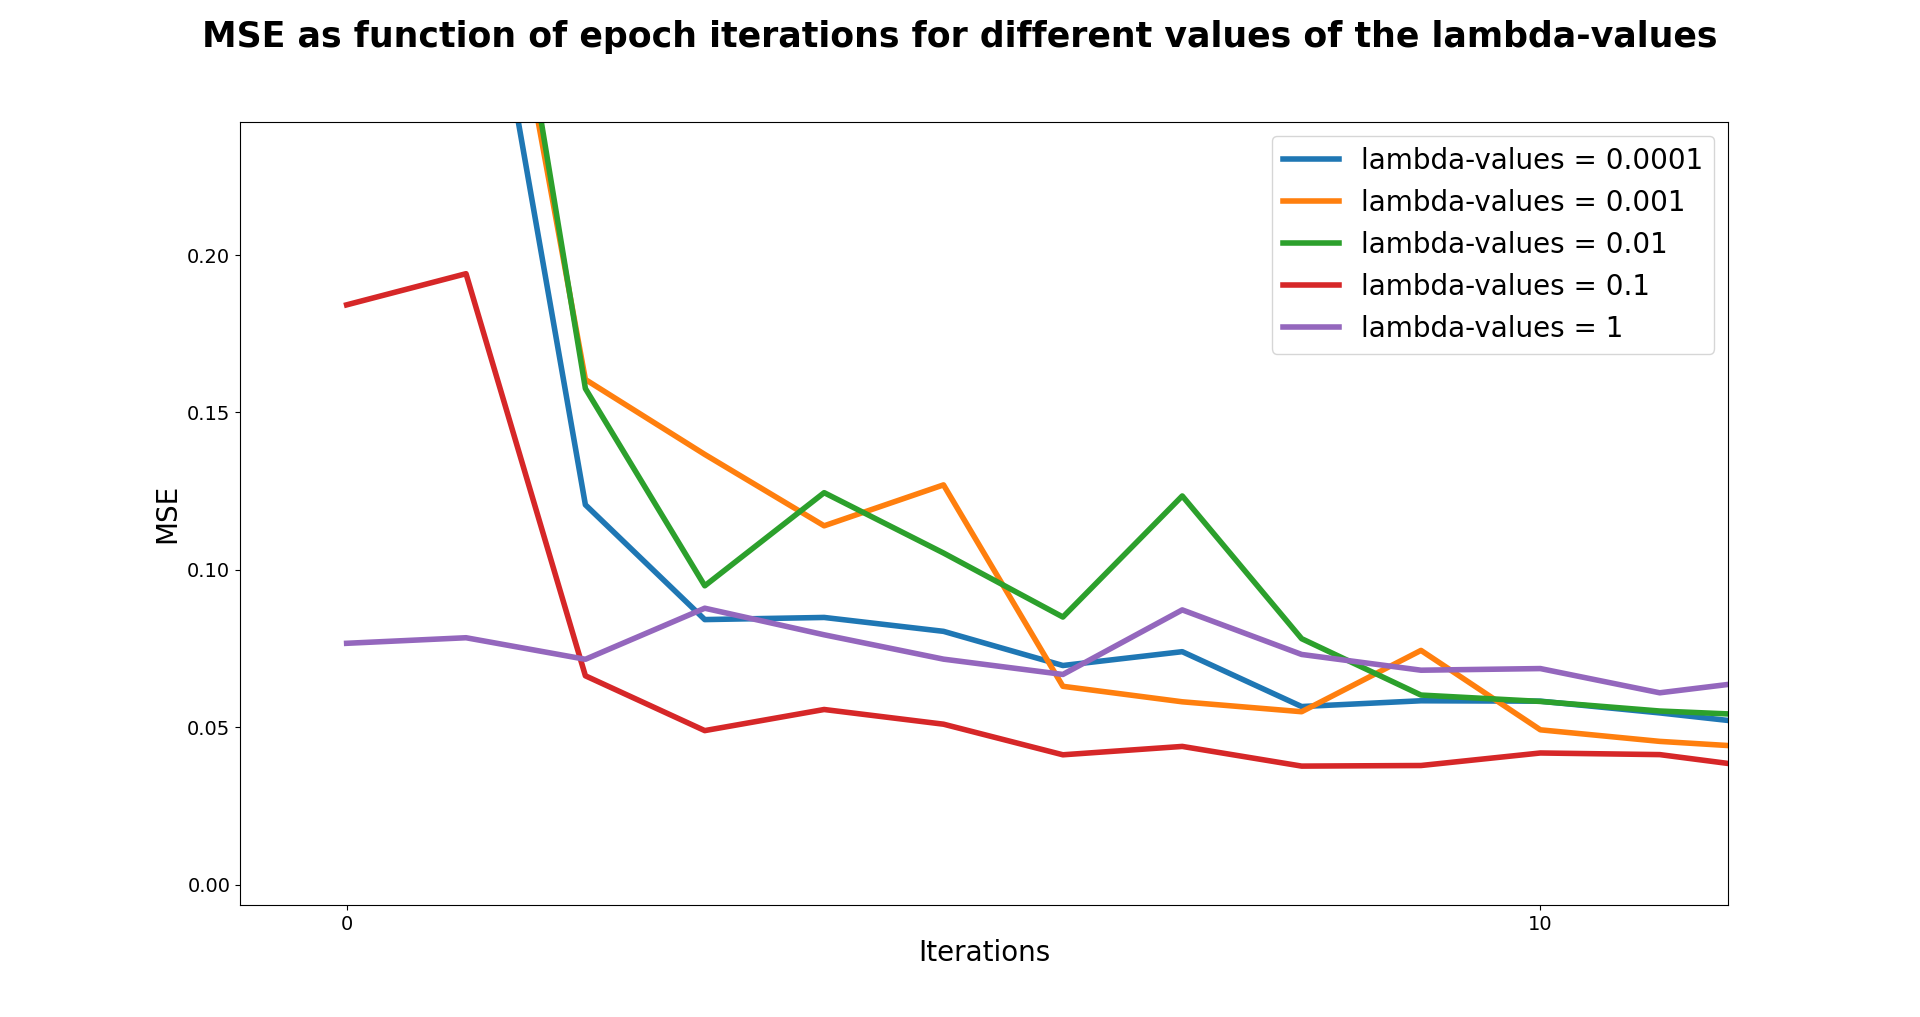
\includegraphics[width = 1\linewidth]{C:/Users/Sander/Documents/GitHub/FYS-STK4155/Project2/Project2/Report/Figures/MSEvsEPOCH_lambRIDGE_schedule2.PNG}
\caption{\label{fig:MSEvsEPOCHlambRIDGE_sch2} The MSE as function of number of epoch iterations and penalty parameter $\lambda$ using a learning schedule and Ridge equivalent SGD. This is a zoom-in of figure \ref{fig:MSEvsEPOCHlambRIDGE_sch}}.
\end{figure}

\noindent We can observe from figures that the choice of penalty parameter $\lambda$ has little or no effect on the MSE, except for when $\lambda = 1$. The MSE in this case never really increase or decrease, which is probably caused by the penalty term setting too many regression coefficients close to zero, meaning there is not really a minimum of the cost function since if all the regression coefficients are to small. 
\\
We also observe that the MSE for penalty parameters less than one decrease their MSE at a very low number of epoch iterations. Indicating that the minimum value is easy to find when some variables are very small.

\newpage

\begin{center}
\Large{\textbf{Exercise 1b)and 1c): Neural network for regression}}
\end{center}

\begin{center}
\large{\textbf{The basics of a neural network}}
\end{center}

\noindent A neural network is a concept based on how neurons operate in the brain where we have an input that travels through neurons that weights the input, eventually making its way to some given set of neuron that trigger an output. This process can be replicated by computers by creating a layered model consisting of one input layer where the data goes in, an output layer where the neural network prediction comes out and a given number of hidden layers consisting of hidden neurons. A conceptual drawing of this process can be seen in figure \ref{fig:nnconcept}

\begin{figure}[H]
\centering
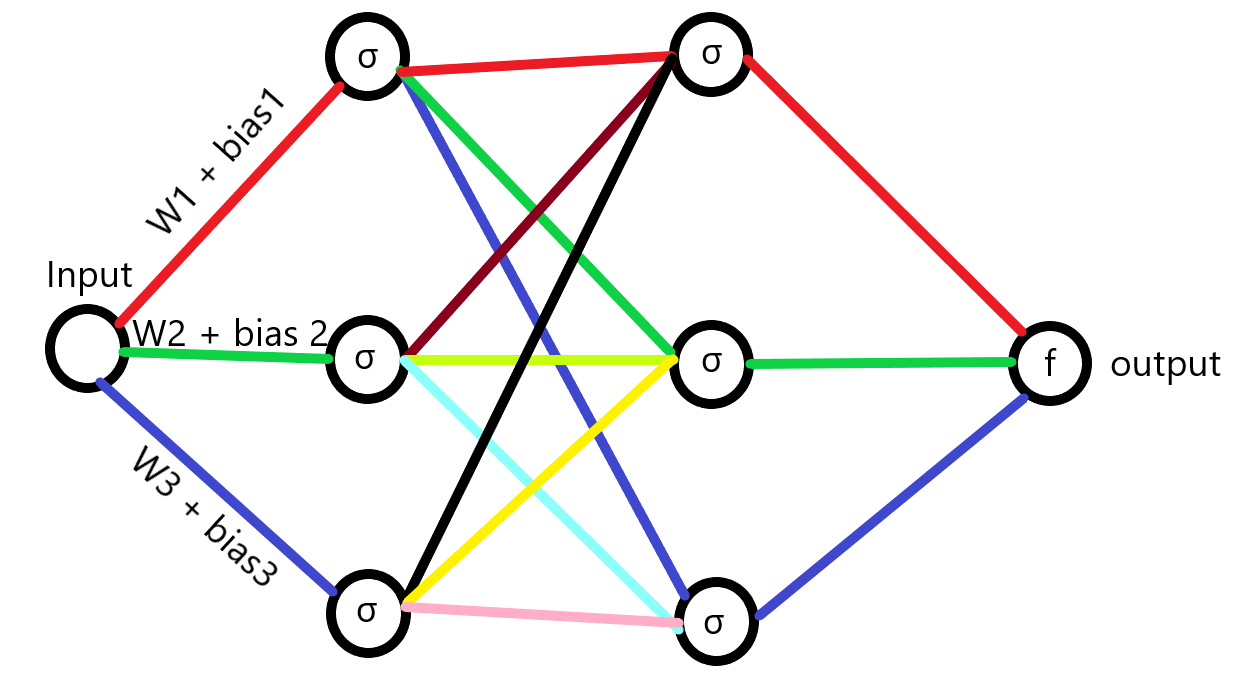
\includegraphics[width = 1\linewidth]{C:/Users/Sander/Documents/GitHub/FYS-STK4155/Project2/Project2/Report/Figures/NeuralNetConcept.PNG}
\caption{\label{fig:nnconcept} Conseptual drawing of a neural network. Here we have one input layer, two hidden layers and one output layer. The input and output layers consist of a single neuron, while the hidden layers have three neurons each. The input to each neuron is a weighted sum (W) plus a bias (B) from the previous layer. The output of a given neuron is the input to that neuron going through a activation function $\sigma$ which is then passed to the neurons in the next layer. The output activation function may be different than that of the neuron activation functions.}
\end{figure}

\noindent Figure \ref{fig:nnconcept} shows an input layer that passes a weighted sum plus bias to the three neurons in the first hidden layer. The weights $W_1, W_2$ and $W_3$ are typically different while the biases $B_1, B_2$ and $B_3$ are typically the equal. When these weighted sums plus bias enter a neuron, they are passed through an activation function which compresses the input to some value between zero and one. It is intuitive to think of this as how activated a neuron is, where one being fully activated and zero being fully inactivated. The data is passed through every neuron in every layer and will eventually reach the output layer where another activation function is applied. This whole process is called feed forward and is typically the first step of any neural network algorithm.
\\
The next step is to tune the weights within the neural network. This is where the gradient descent from exercise 1a) comes in. We can utilize the stochastic gradient descent to find the minimum of a cost function where each dimension is the weights of the neural network. Can then find which value of the weight would incrementally decrease the cost function, and then go back though our neural network and update the weight values in each neuron. This process is often called back propagation. We want to repeat the feed forward and back propagation many times in order for the weight to find their optimal value. This is called the training of the neural network. When we have trained the neural network sufficiently, it can be used to predict new data the network has never seen before. With these processes in mind, we can implement an algorithm that performs feed forward and back propagation.

\begin{center}
\large{\textbf{The sigmoid activation function}}
\end{center}

\noindent Three types of activation functions within the hidden layers will be implemented, the first one being the sigmoid activation function which is given by equation \ref{eq:sig}

\begin{equation}\label{eq:sig}
\begin{aligned}
\frac{1}{1 + e^{-x}}
\end{aligned}
\end{equation}

\noindent It can be seen from the definition of the sigmoid function that whatever the value of x, the output is always somewhere between zero and one. We can utilize this to force the neurons to output a value between zero and one.

\begin{center}
\large{\textbf{The RELU activation functions}}
\end{center}

\noindent So far we have only utilized the sigmoid function in our hidden neurons as defined in equation \ref{eq:sig}. Now we want to experiment with two additional activation functions, namely the RELU and the leaky RELU defined in equation \ref{eq:RELU} and \ref{eq:leakyRELU}

\begin{equation}\label{eq:RELU}
\begin{aligned}
f(x) = 
\begin{cases}
x,& \text{if } x > 0\\
0,& \text{otherwise}
\end{cases}
\end{aligned}
\end{equation}

\begin{equation}\label{eq:leakyRELU}
\begin{aligned}
f(x) = 
\begin{cases}
x,& \text{if } x > 0\\
ax,& \text{otherwise}
\end{cases}
\end{aligned}
\end{equation}

\noindent We can see that this is close to the linear activation function where the input is simply passed through without any alterations. However, if the input is zero, then the output from a given neuron will be zero in the RELU case. The same goes for the leaky RELU case, but instead if setting the input values to zero, we set it to some small constant times the input. a in equation \ref{eq:leakyRELU} is typically in the range of $0.01$ and kind of has the same purpose as the bias in the way that it prevents the neuron from ever giving an output of zero (thereby the name "leaky"). Similar to the bias, this is done to prevent a chain of zeros to be passed through the neural network.
\\
One can observe from equations \ref{eq:RELU} and \ref{eq:leakyRELU} that the output from a given neuron will not be between zero and one if the input to the neuron is greater than zero. This has proven to be a problem when implementing the code as some configurations of the neural network will explode the gradient. The exploding gradient happens when 
\\
We can now perform the same analysis as in exercise 1b), but using the RELU and leaky RELU instead of the sigmoid as our hidden layer activation function.

\begin{center}
\large{\textbf{Learning rate, weights and biases}}
\end{center}

\noindent The neural network have proved stable when using the sigmoid activation function for the hidden layers as observed from the previous exercise. The leaky RELU and sometimes the RELU were prone to overflow leading to a worse predictions. The overflow became a huge problem for learning rates larger than 0.01, and therefore, only learning rates under this value were considered. Another solution to counter the overflow problem were increasing the number of epoch iterations to 2000 and decreasing the batch size to around 5. 
\\
It was also observed that the initial weights really impacted whether the network overflowed or not. Setting the initial weight to some random number drawn from a standard normal distribution gave severe flaws for many layer/neuron configurations. However, the xavier weight initialization proved to stabilize the network in most cases. The xavier weight initialization aims to maintain a constant variance of the data passing through the network (kilde). Doing this drastically reduced the chance for overflow which really showed when coding the network.
\\
The bias has in this case was simply been set to $0.01$. The role of the bias is to make sure there is some input to the neurons. Say a neuron only receives zeros from the previous layer. This would in turn lead to a feed forward of only zeros for that particular set of neurons meaning they will never contribute to the network. Therefore, it is important to add some bias to each neuron. The choice of bias showed to be of little significance when we played around with the code. The only important thing was that the bias was greater than zero, as a bias of zero often resulted in the network only passing zeros through, ultimately leading to a terrible prediction.

\begin{center}
\large{\textbf{Neural network results}}
\end{center}

\noindent We first want to see how the different activation function behave relative to the number of epoch iterations, the size of the batch and the learning rate. Figure \ref{fig:MSEvsLrateTOTAL1} and \ref{fig:MSEvsLrateTOTAL2} show the MSE and $R^2$ as function of learning rate using 100 epoch iterations and a batch size of 10 for the sigmoid, RELU and leaky RELU activation functions

\begin{figure}[H]
\centering
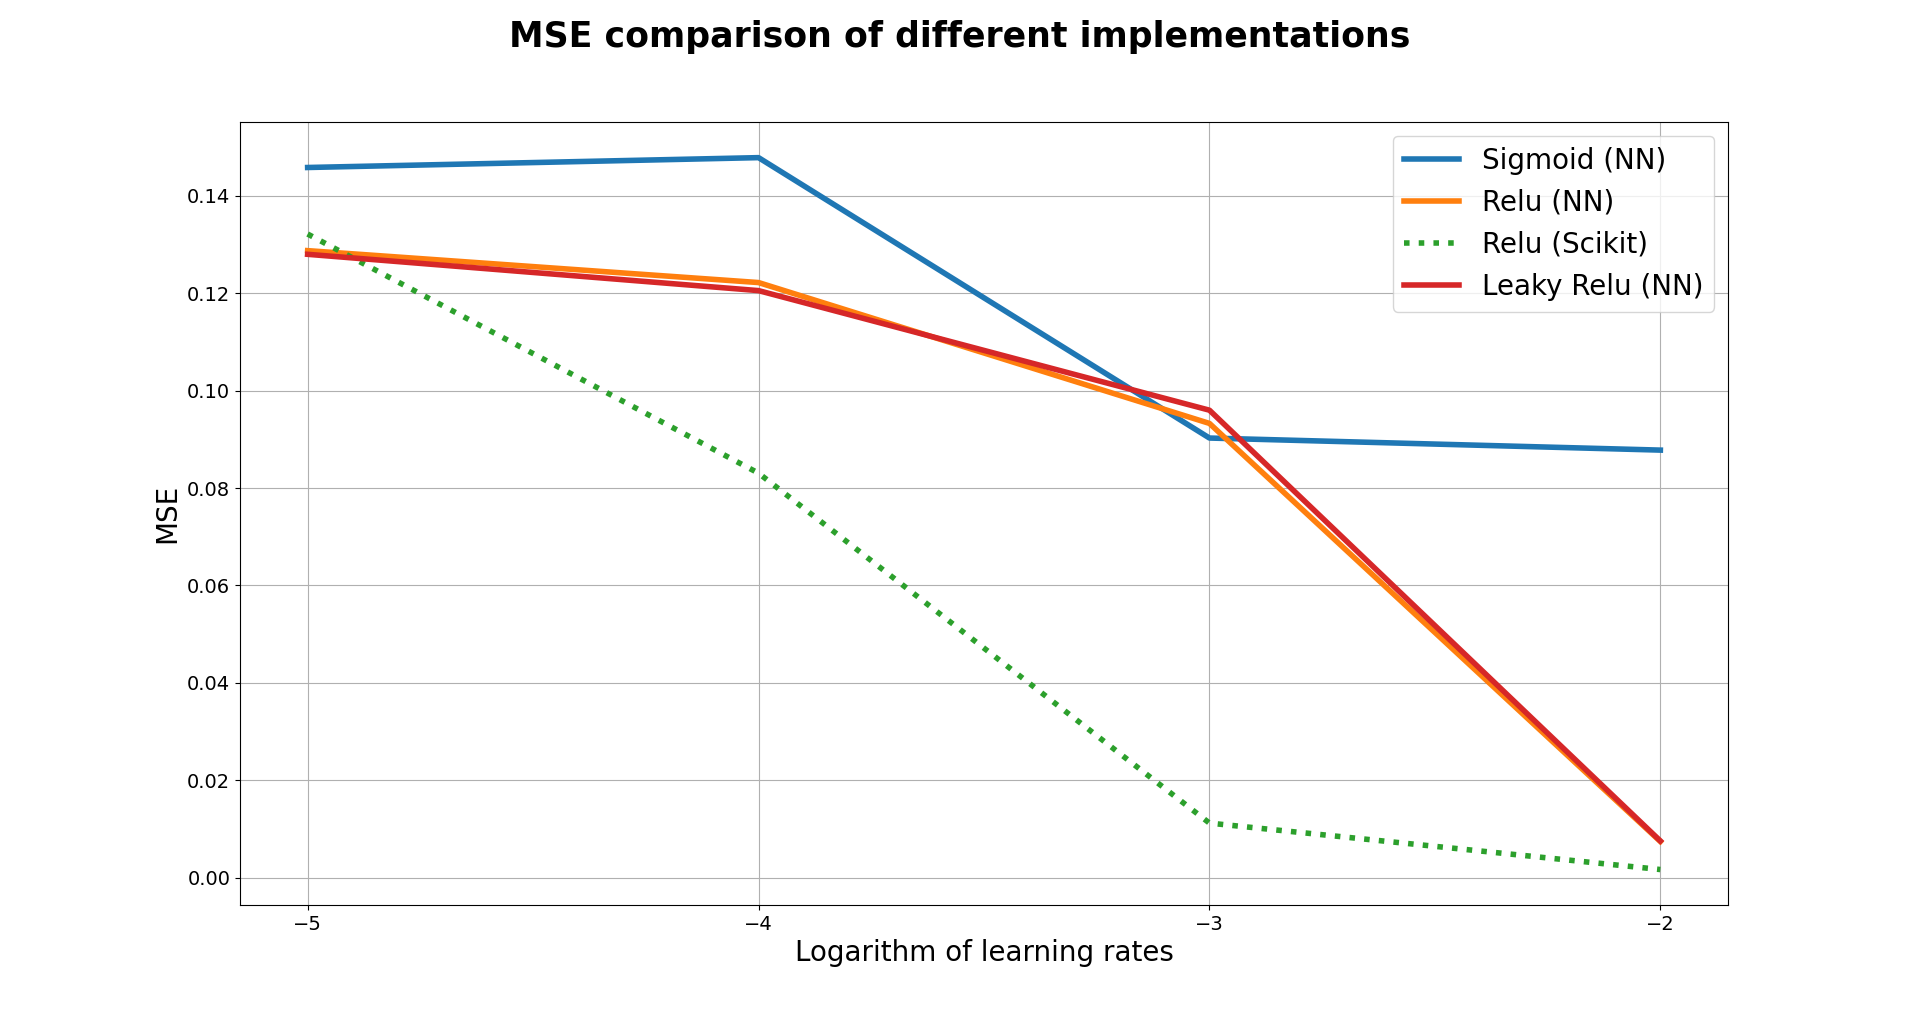
\includegraphics[width = 1\linewidth]{C:/Users/Sander/Documents/GitHub/FYS-STK4155/Project2/Project2/Report/Figures/MSEvsLearn_OLS_TOTAL_epoch100_batch10.PNG}
\caption{\label{fig:MSEvsLrateTOTAL1} The MSE as function of number of learning rate for the three activation functions when we utilize 100 epoch iterations and a batch size of 10. This is the OLS equivalent.}
\end{figure}

\begin{figure}[H]
\centering
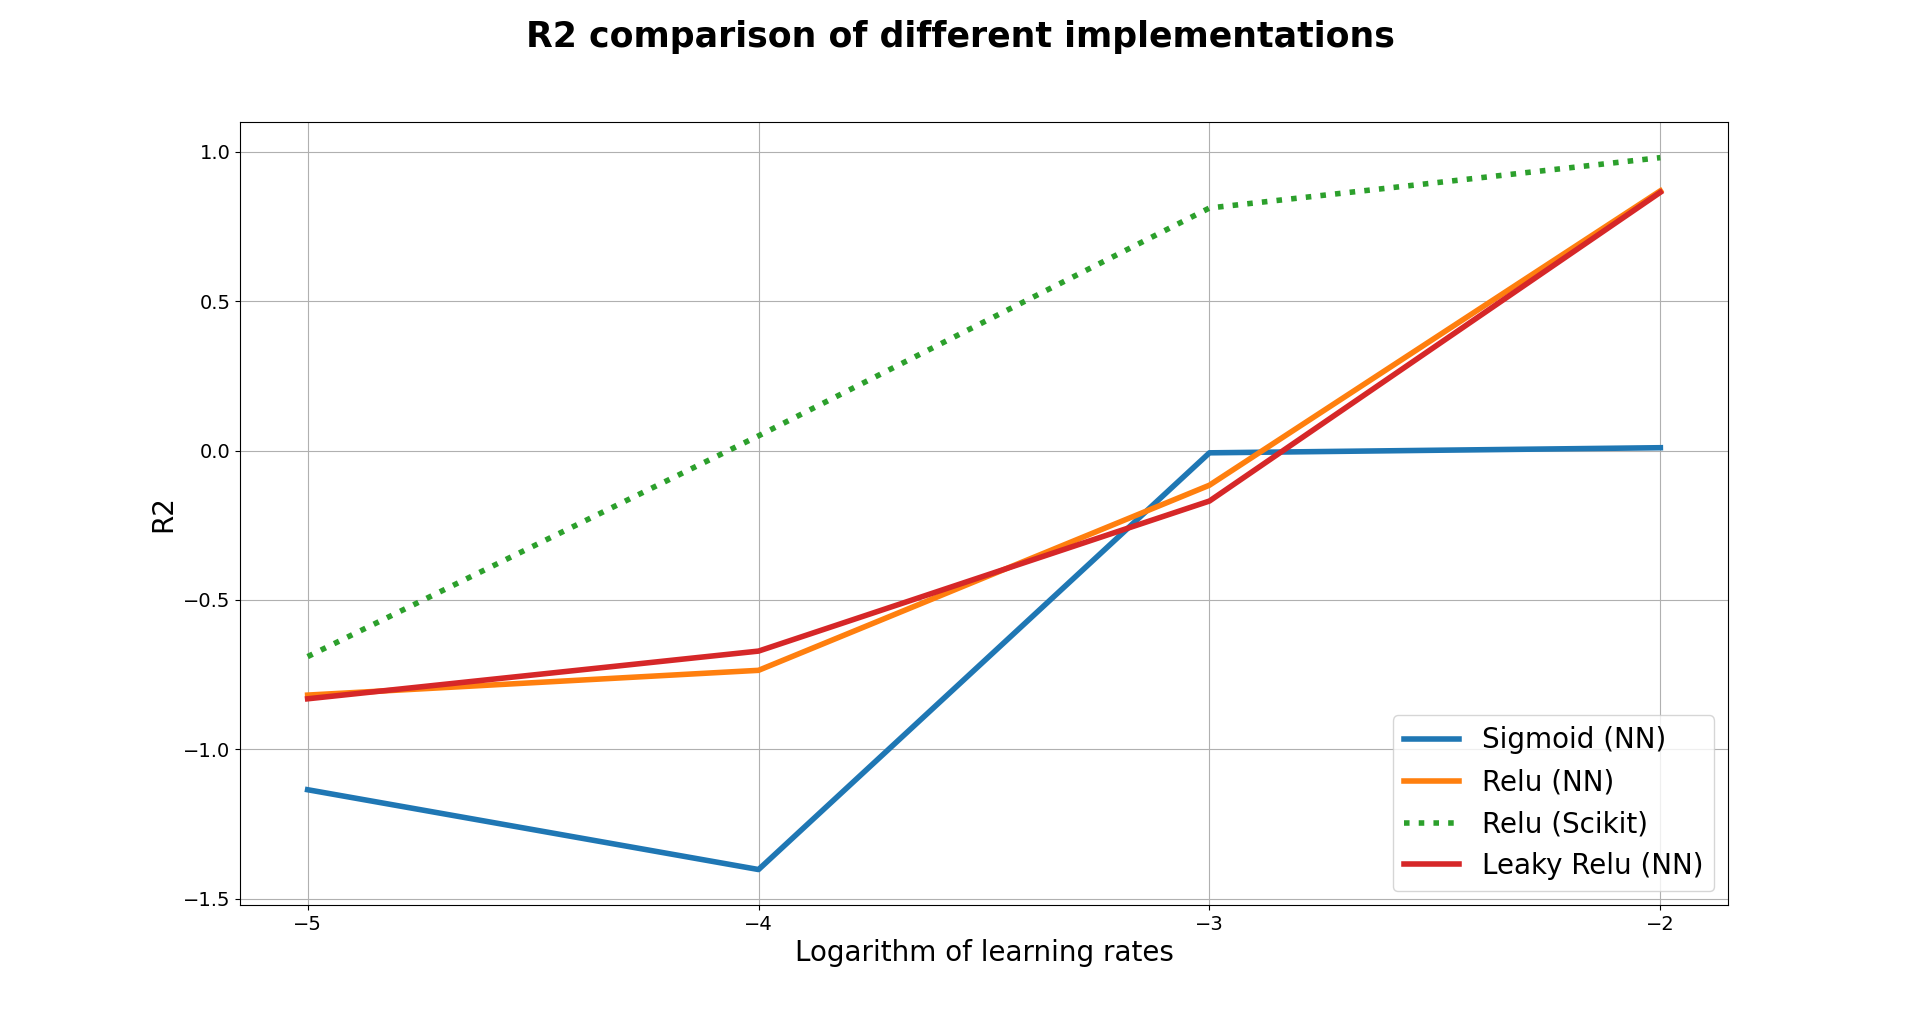
\includegraphics[width = 1\linewidth]{C:/Users/Sander/Documents/GitHub/FYS-STK4155/Project2/Project2/Report/Figures/MSEvsLearn_OLS_TOTAL_epoch100_batch10_r2.PNG}
\caption{\label{fig:MSEvsLrateTOTAL2} The $R^2$ as function of number of learning rate for the three activation functions when we utilize 100 epoch iterations and a batch size of 10. This is the OLS equivalent.}
\end{figure}

\noindent Figures \ref{fig:MSEvsLrateTOTAL1} and \ref{fig:MSEvsLrateTOTAL2} also include the Scikit implementation of the RELU activation function. It can be observed that the Scikit implementation outperforms my own neural network, particularly for lower learning rates. My own RELU and leaky RELU implementations seem nearly equivalent and are able to predict the test set much better than the sigmoid. It seems that the sigmoid implementation reaches a cap at $R^2 = 0$, which is equivalent to the baseline model. This means that the sigmoid model is just as good as randomly guessing the prediction. It can also be observed that the RELU implementations gets closer to the Scikit implementation for higher learning rates. We now aim to increase the number of epoch iterations from 100 to 500 as seen in figures \ref{fig:MSEvsLrateTOTAL3} and \ref{fig:MSEvsLrateTOTAL4}

\begin{figure}[H]
\centering
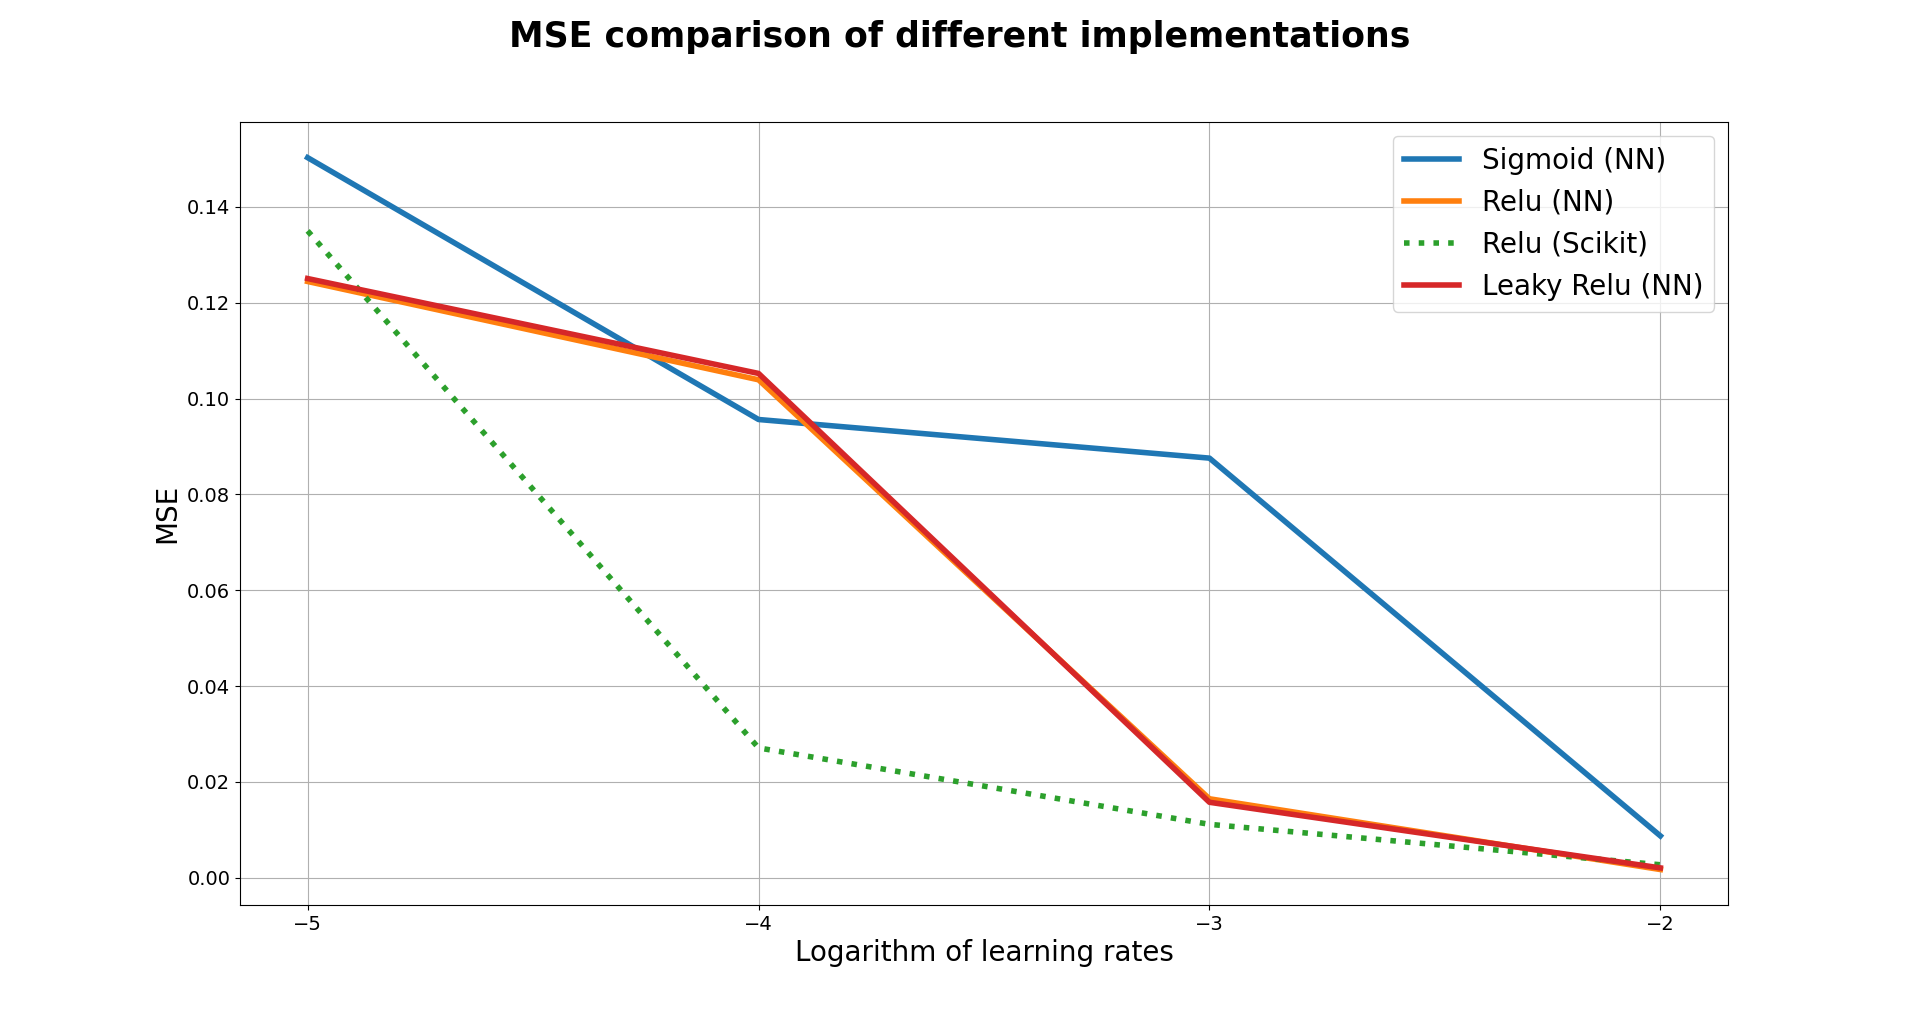
\includegraphics[width = 1\linewidth]{C:/Users/Sander/Documents/GitHub/FYS-STK4155/Project2/Project2/Report/Figures/MSEvsLearn_OLS_TOTAL_epoch500_batch10.PNG}
\caption{\label{fig:MSEvsLrateTOTAL3} The MSE as function of number of learning rate for the three activation functions when we utilize 500 epoch iterations and a batch size of 10. This is the OLS equivalent.}
\end{figure}

\begin{figure}[H]
\centering
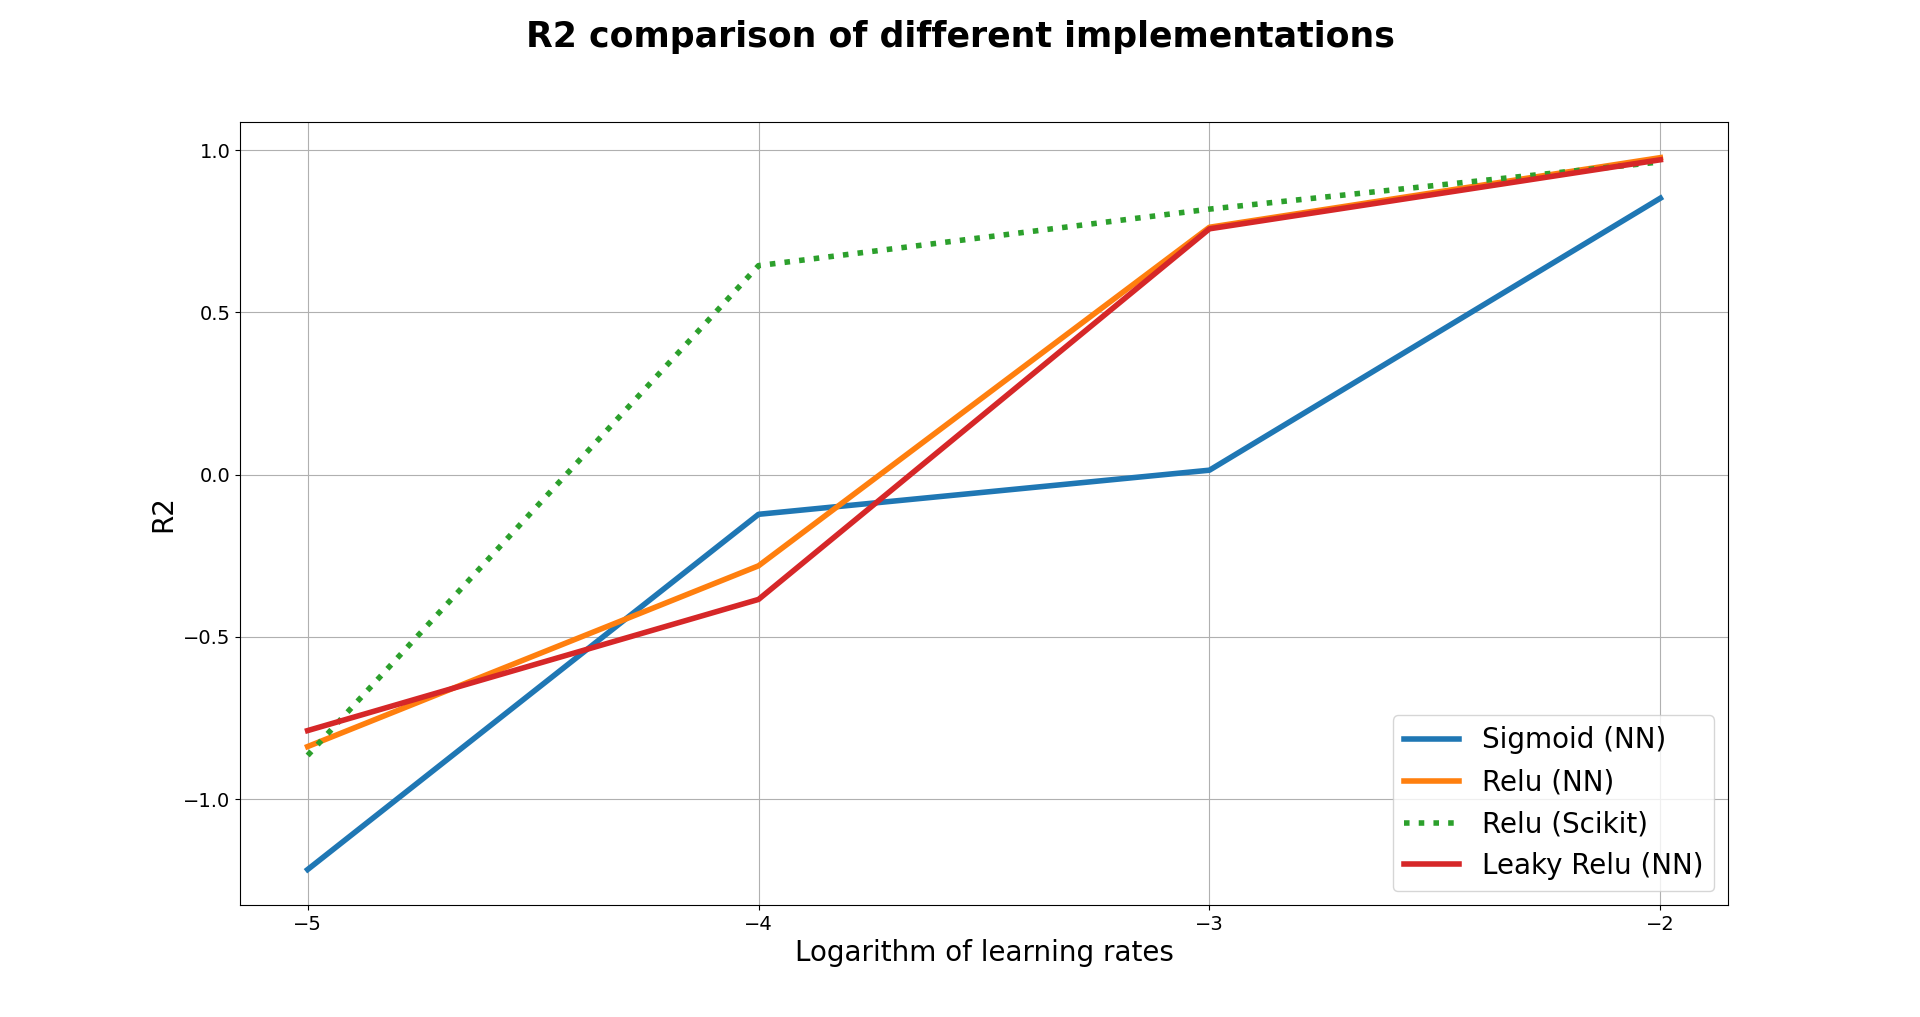
\includegraphics[width = 1\linewidth]{C:/Users/Sander/Documents/GitHub/FYS-STK4155/Project2/Project2/Report/Figures/MSEvsLearn_OLS_TOTAL_epoch500_batch10_r2.PNG}
\caption{\label{fig:MSEvsLrateTOTAL4} The $R^2$ as function of number of learning rate for the three activation functions when we utilize 500 epoch iterations and a batch size of 10. This is the OLS equivalent.}
\end{figure}

\noindent One can observe that increasing the number of epoch iterations caused the sigmoid implementation to perform better. It seems as going over some epoch threshold results in the sigmoid implementation breaking through the previously stated cap and it can therefore predict the test data better than the baseline. We now increase the number of epoch iterations from 500 to 2000 as seen in figures \ref{fig:MSEvsLrateTOTAL5} and \ref{fig:MSEvsLrateTOTAL6}

\begin{figure}[H]
\centering
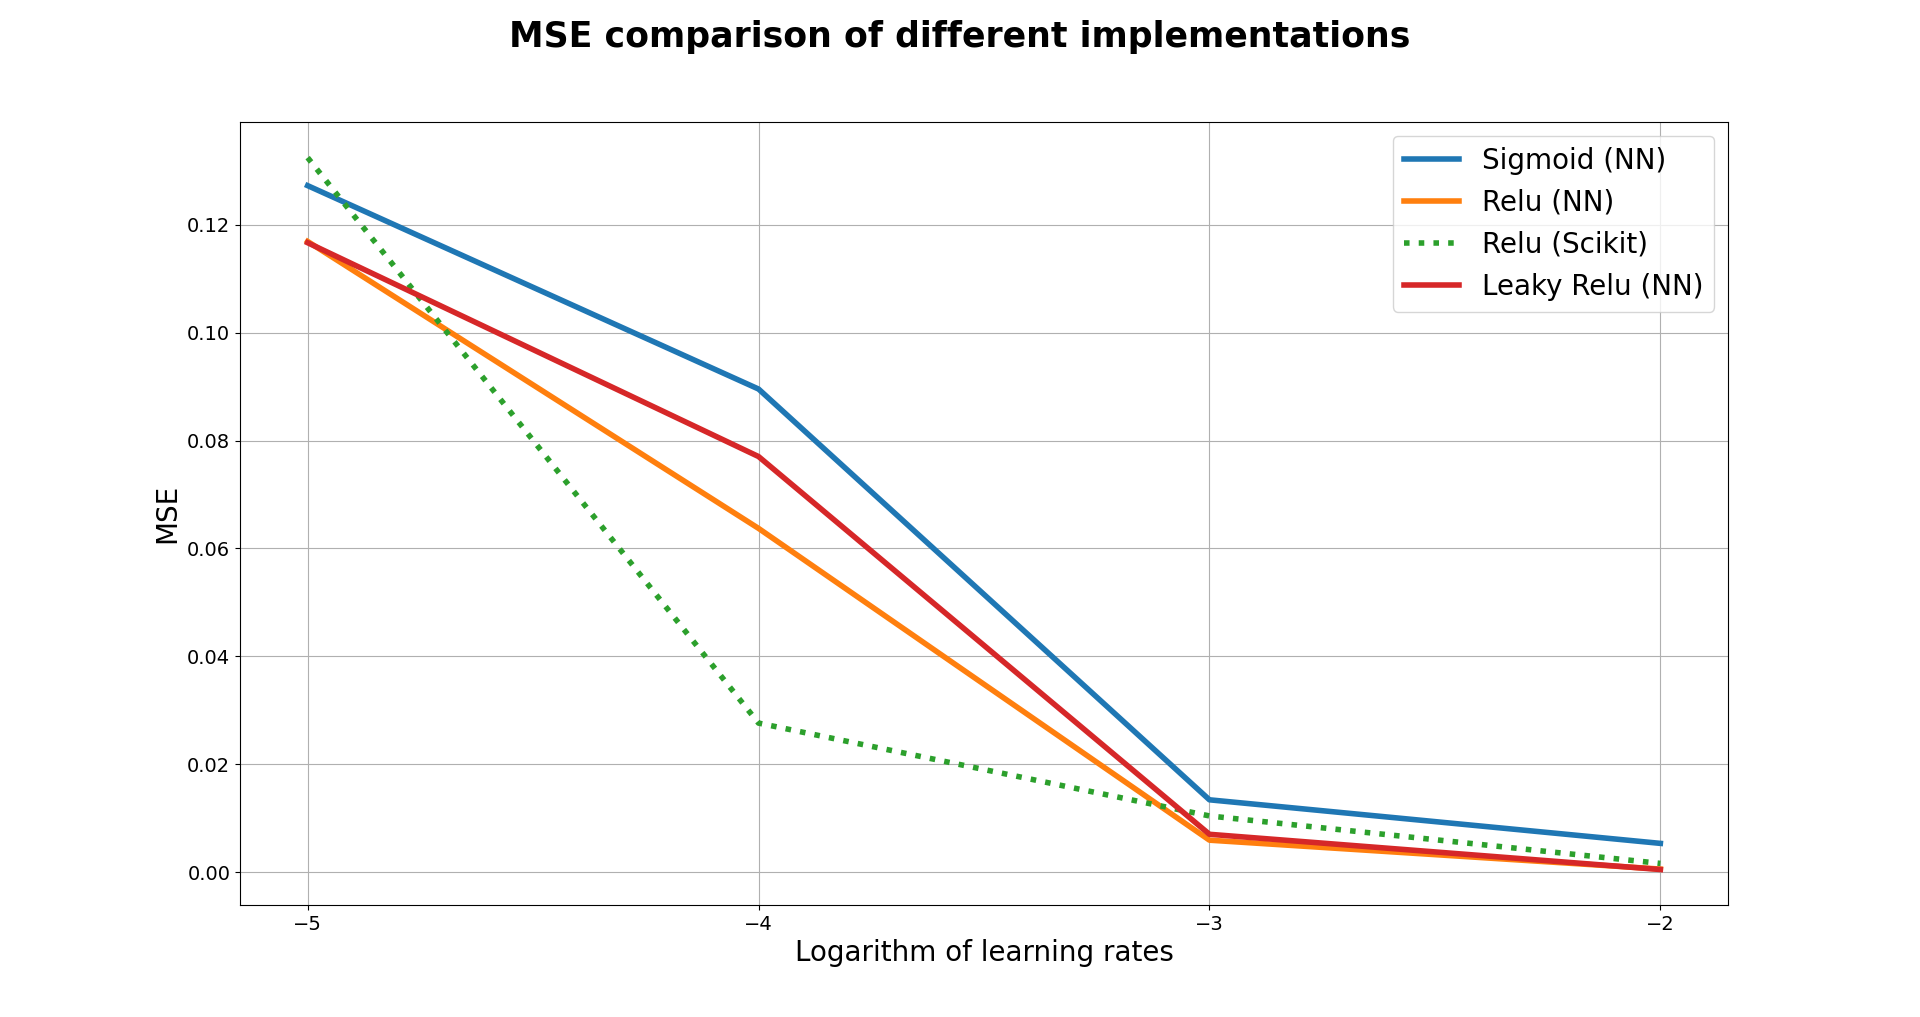
\includegraphics[width = 1\linewidth]{C:/Users/Sander/Documents/GitHub/FYS-STK4155/Project2/Project2/Report/Figures/MSEvsLearn_OLS_TOTAL_epoch2000_batch10.PNG}
\caption{\label{fig:MSEvsLrateTOTAL5} The MSE as function of number of learning rate for the three activation functions when we utilize 2000 epoch iterations and a batch size of 10. This is the OLS equivalent.}
\end{figure}

\begin{figure}[H]
\centering
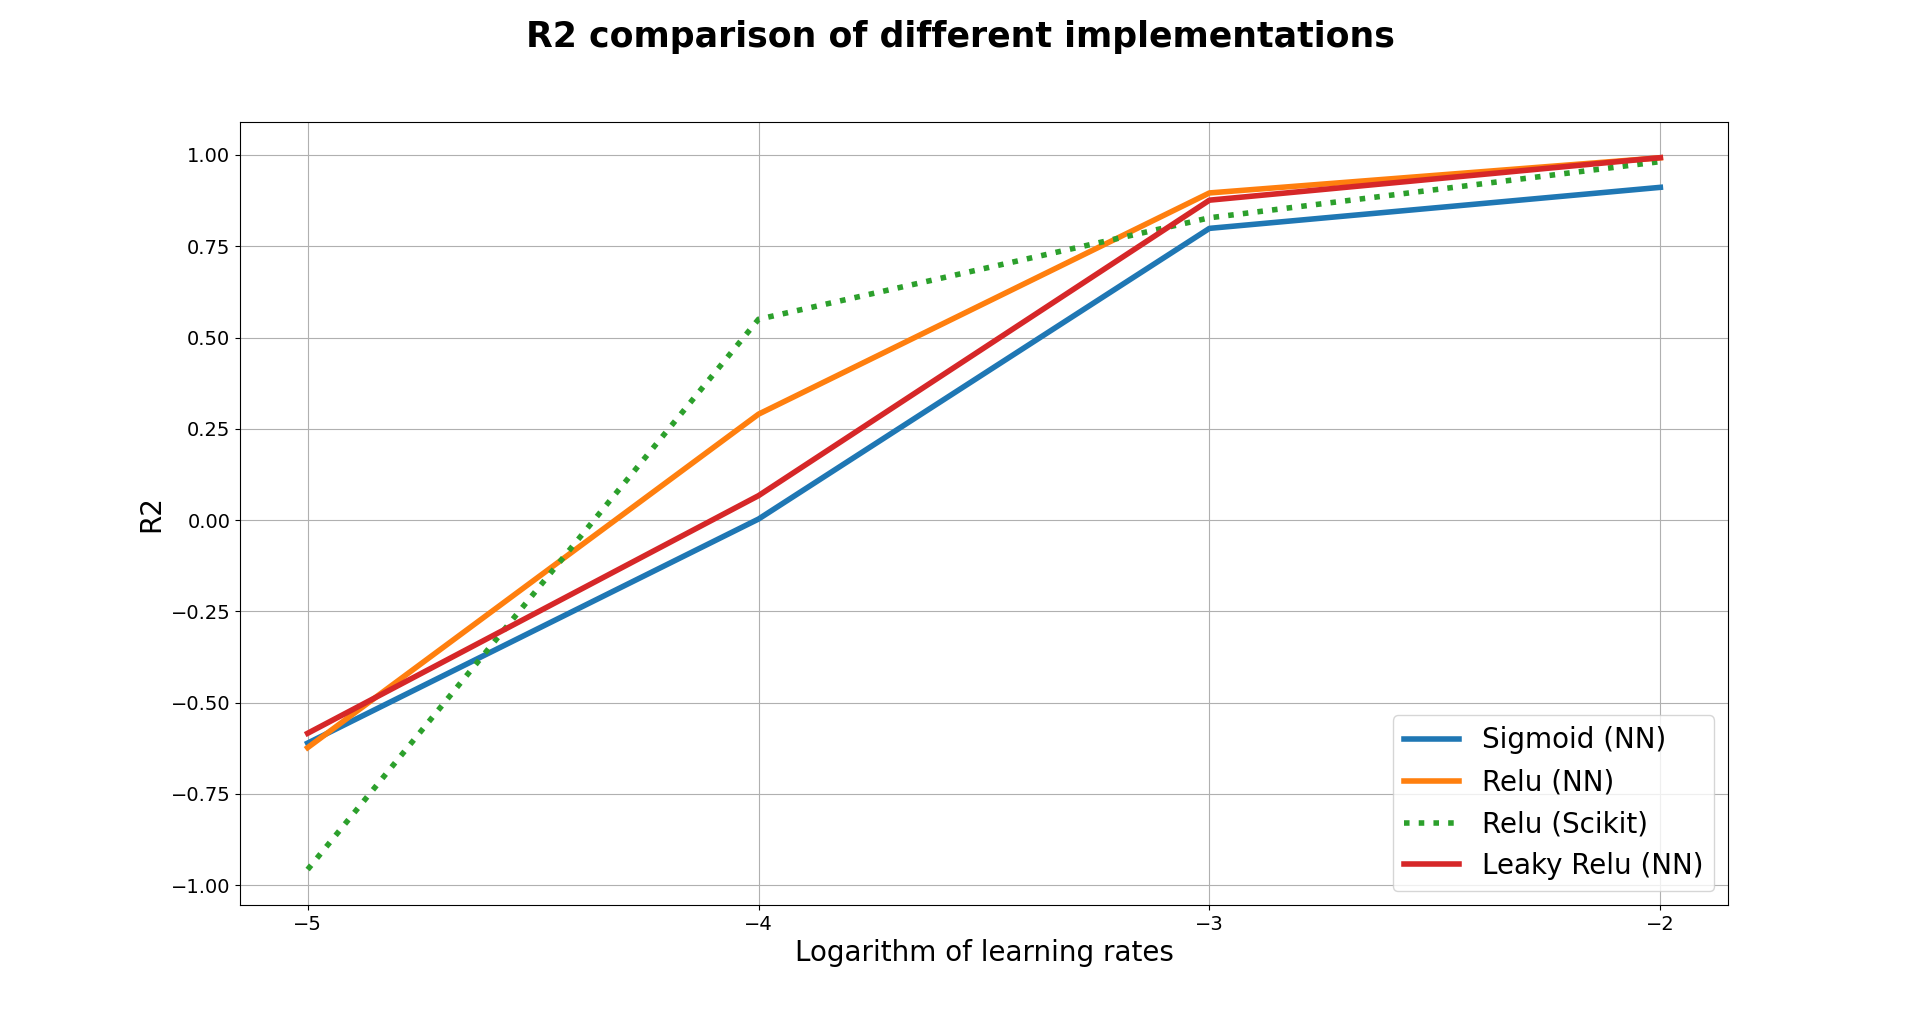
\includegraphics[width = 1\linewidth]{C:/Users/Sander/Documents/GitHub/FYS-STK4155/Project2/Project2/Report/Figures/MSEvsLearn_OLS_TOTAL_epoch2000_batch10_r2.PNG}
\caption{\label{fig:MSEvsLrateTOTAL6} The $R^2$ as function of number of learning rate for the three activation functions when we utilize 2000 epoch iterations and a batch size of 10. This is the OLS equivalent.}
\end{figure}

\noindent One can observe from figures \ref{fig:MSEvsLrateTOTAL5} and \ref{fig:MSEvsLrateTOTAL6} that the three implementations now perform about the same. This leads one to believe that there is a given threshold for when the activation functions are equivalent. At learning rates higher than 0.001, my implementations performs on par with the Scikit implementation, which is reassuring. 
\\
We now aim to see the variation in term of the size of the batch. We keep the number of epochs at 2000, but decrease the batch size from 10 to 2. Figures QQQ and QQQ shows these results.

\begin{figure}[H]
\centering
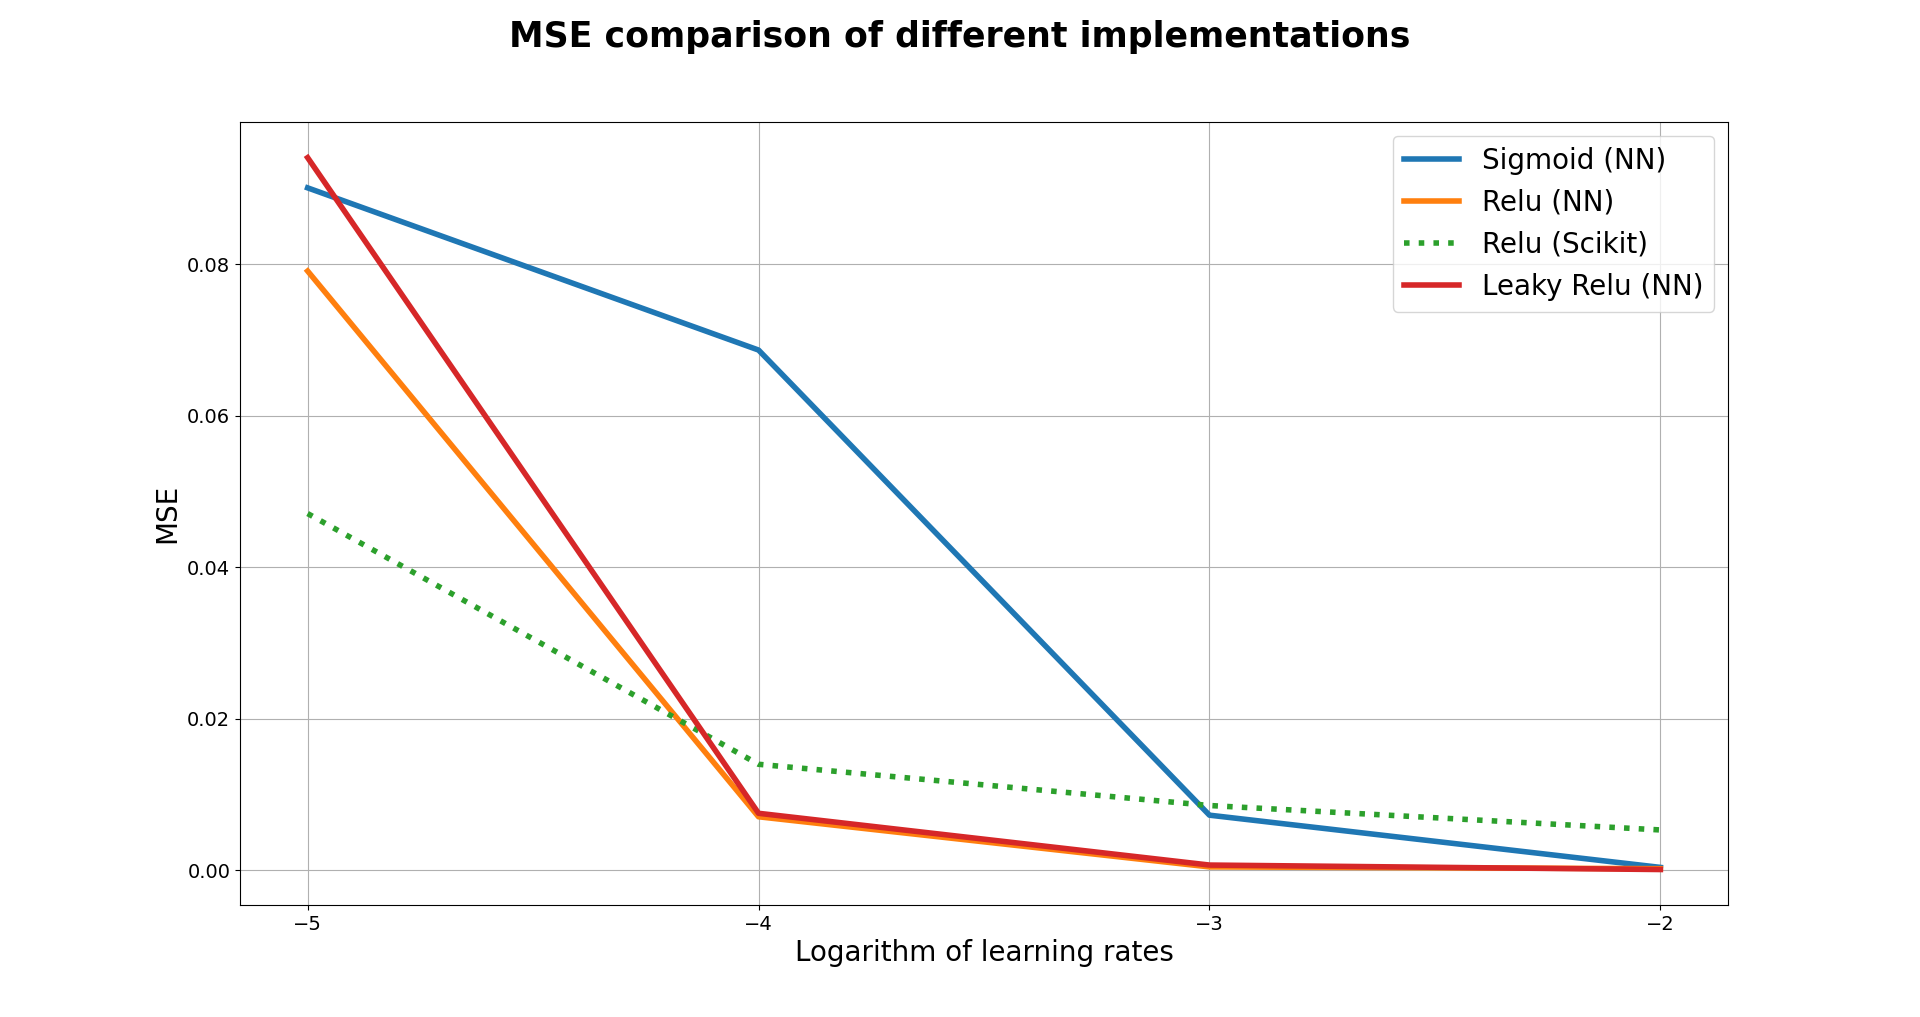
\includegraphics[width = 1\linewidth]{C:/Users/Sander/Documents/GitHub/FYS-STK4155/Project2/Project2/Report/Figures/MSEvsLearn_OLS_TOTAL_epoch2000_batch2.PNG}
\caption{\label{fig:MSEvsLrateTOTAL7} The MSE as function of number of learning rate for the three activation functions when we utilize 2000 epoch iterations and a batch size of 2. This is the OLS equivalent.}
\end{figure}

\begin{figure}[H]
\centering
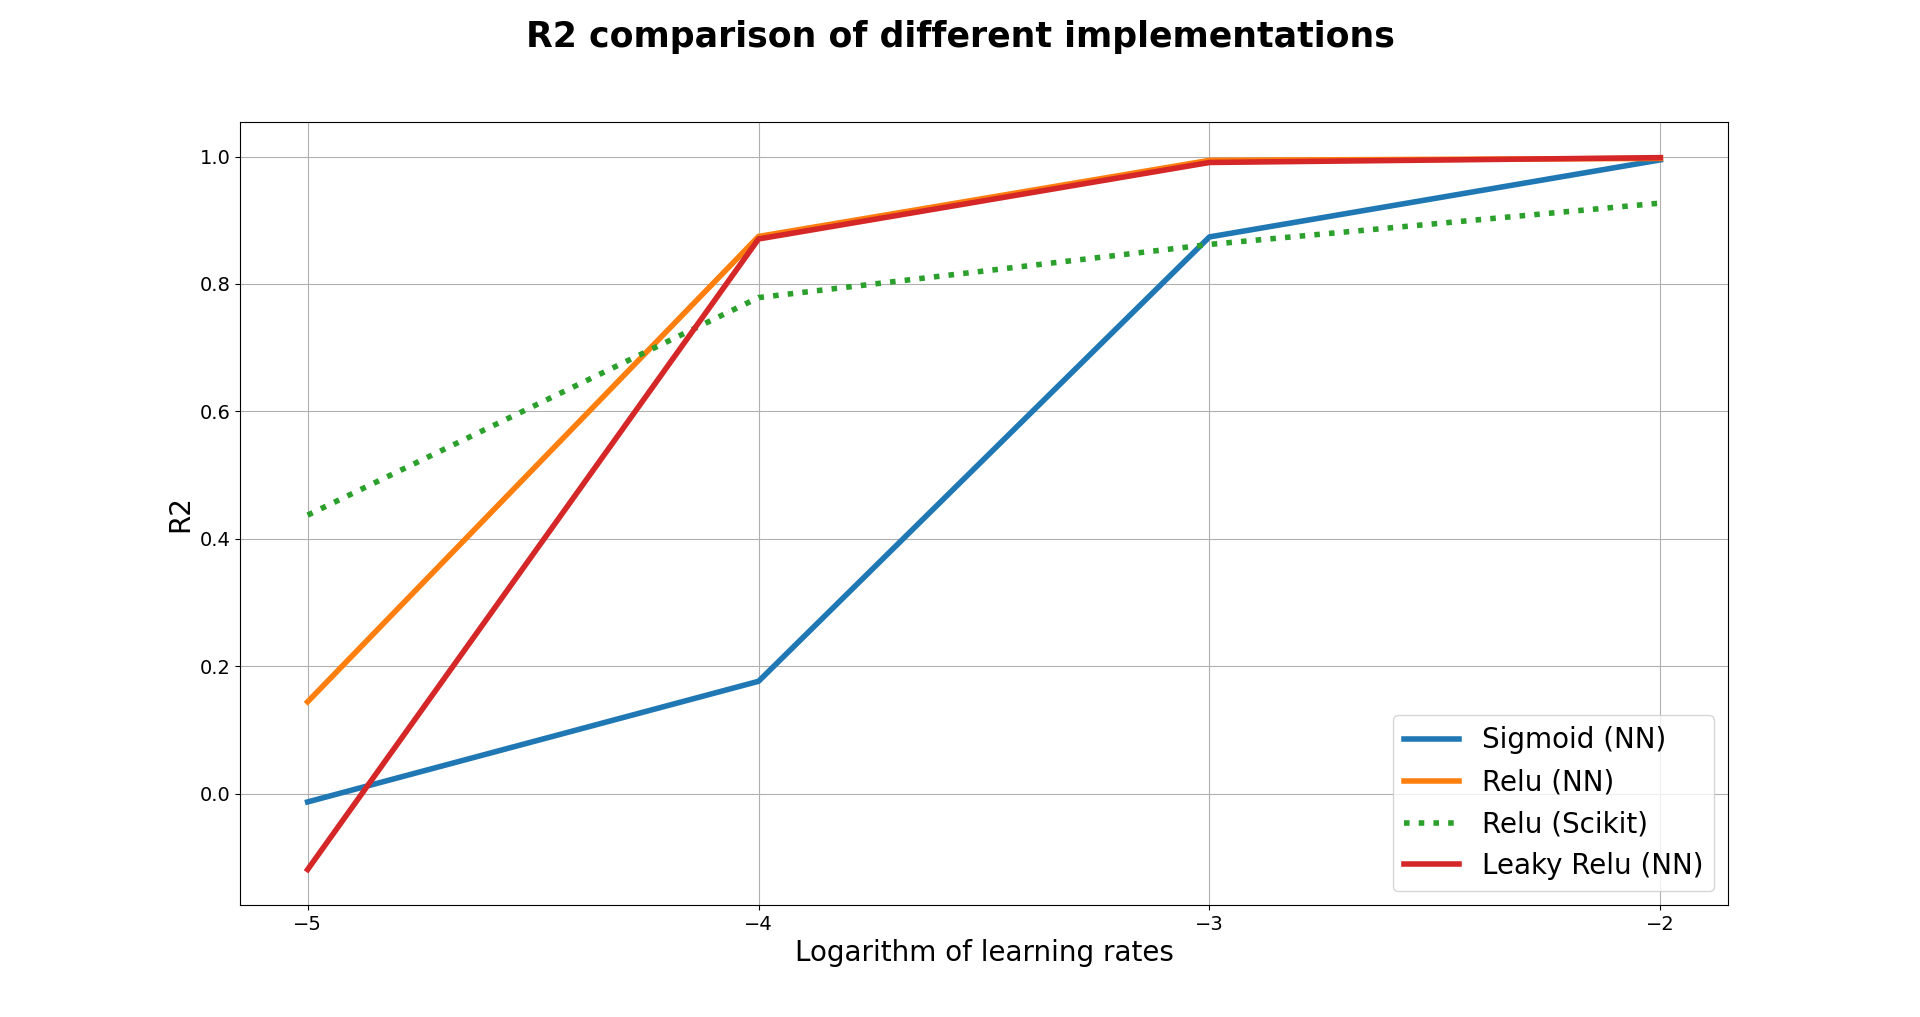
\includegraphics[width = 1\linewidth]{C:/Users/Sander/Documents/GitHub/FYS-STK4155/Project2/Project2/Report/Figures/MSEvsLearn_OLS_TOTAL_epoch2000_batch2_r2.PNG}
\caption{\label{fig:MSEvsLrateTOTAL8} The $R^2$ as function of number of learning rate for the three activation functions when we utilize 2000 epoch iterations and a batch size of 2. This is the OLS equivalent.}
\end{figure}

\noindent One can observe that the decreasing the batch size does not really impact the Scikit and sigmoid implementations, but the RELU implementations are severely improved. In fact, the RELU implementations outperform the Scikit implementations at learning rates over 0.0001. Additionally, my own implementations outperform the Scikit implementations for learning rates higher than 0.001.
\\
We now see that increasing the number of epoch and decreasing the batch size leads to better prediction for my own neural network implementations. The next goal is to find the number of hidden layers and hidden neurons that minimize the MSE (or maximize the $R^2$). To do this, we implement the different activation functions using 2000 epoch iterations and a batch size of 2. Then, we can plot a heatmap where we study the MSE as function of the number of hidden layers and hidden neurons. We only consider hidden layers between 1 and 10 and hidden neurons between 1 and 100, as this task is extremely computationally heavy using 2000 epoch iterations and a batch size of 2. The MSE heatmap using the sigmoid activation function can be seen in figure \ref{fig:heatmap1}

\begin{figure}[H]
\centering
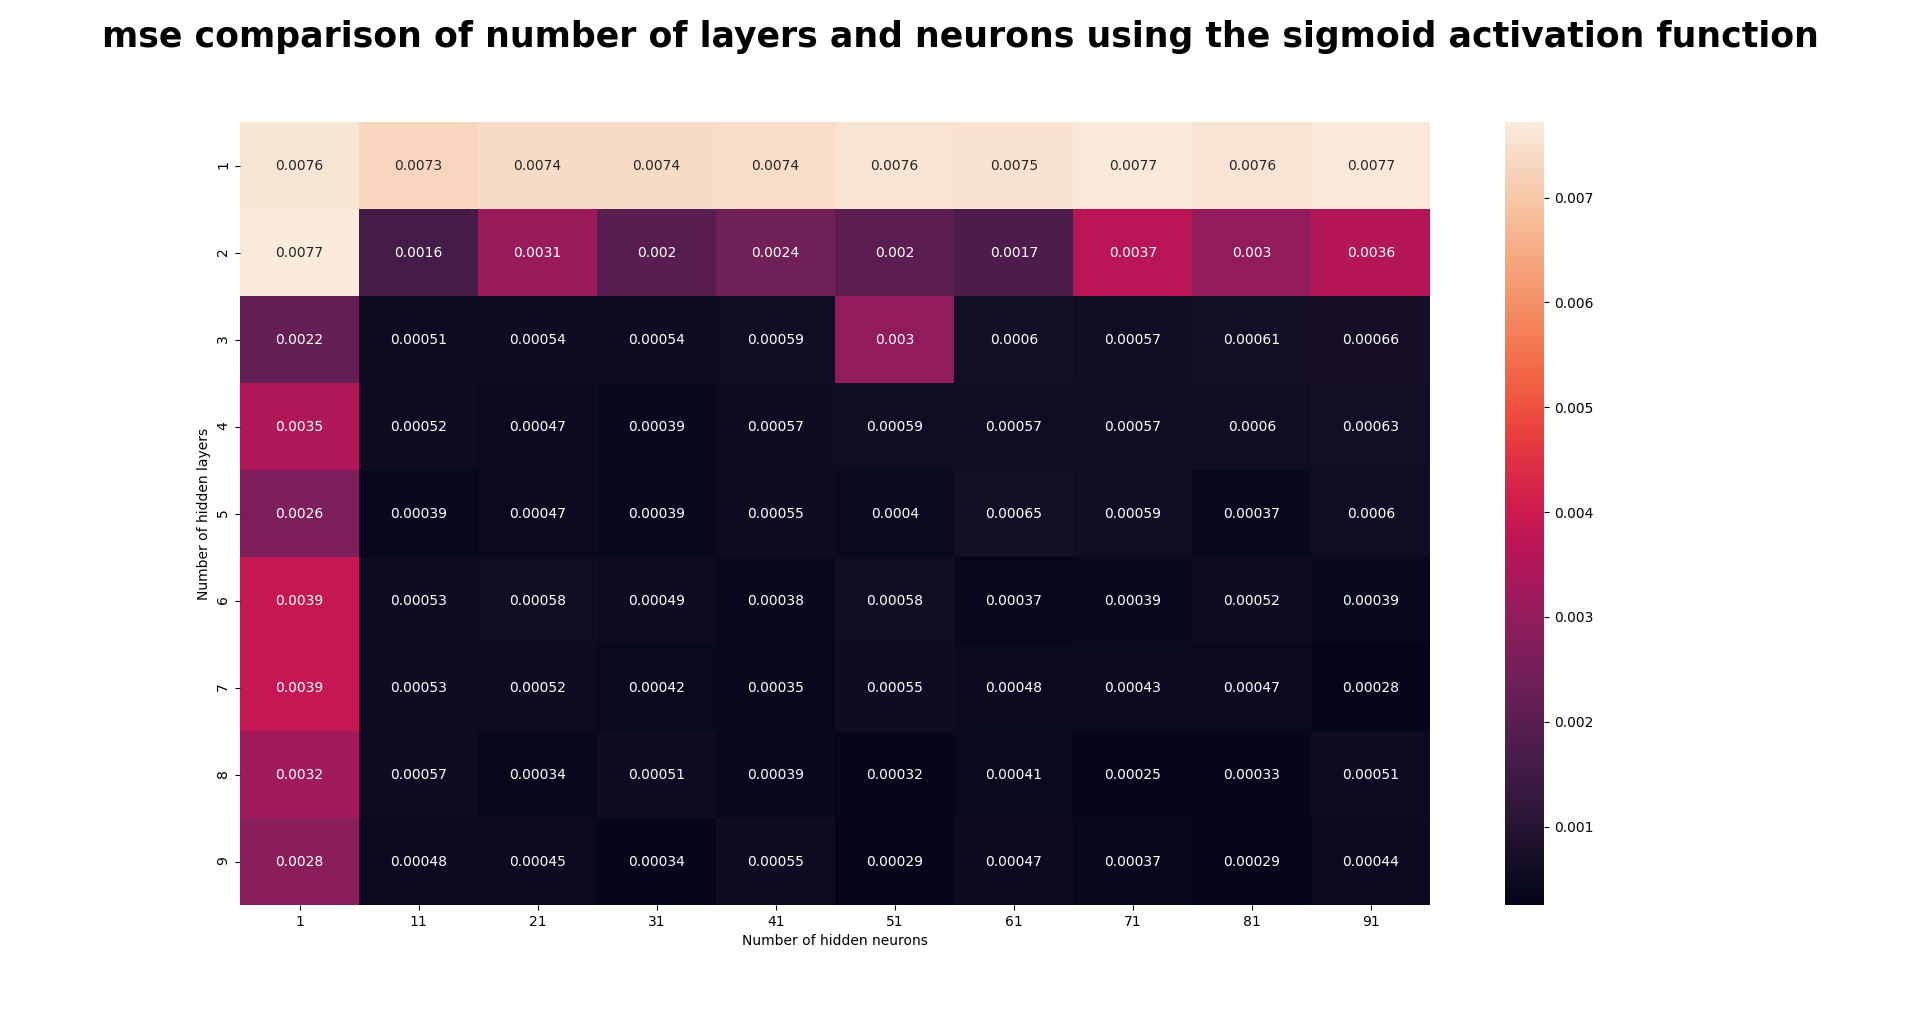
\includegraphics[width = 1\linewidth]{C:/Users/Sander/Documents/GitHub/FYS-STK4155/Project2/Project2/Report/Figures/heatmapOLS_TOTAL_sigmoidMSE_REAL.PNG}
\caption{\label{fig:heatmap1} Heatmap for different number of hidden layers and neurons using the sigmoid activation function. This is the OLS equivalent.}
\end{figure}

\noindent One can observe from the heatmap in figure \ref{fig:heatmap1} that the neural network performs well as long as we keep the number of hidden layers above 4 and the number of hidden neurons above 10. In this range, the MSE is less than $0.0006$ which means the network is able to predict the Franke function accurately. Let us now take a look at the RELU implementation using both my own and the Scikit implementation as seen in figures QQQ and QQQ.

\begin{figure}[H]
\centering
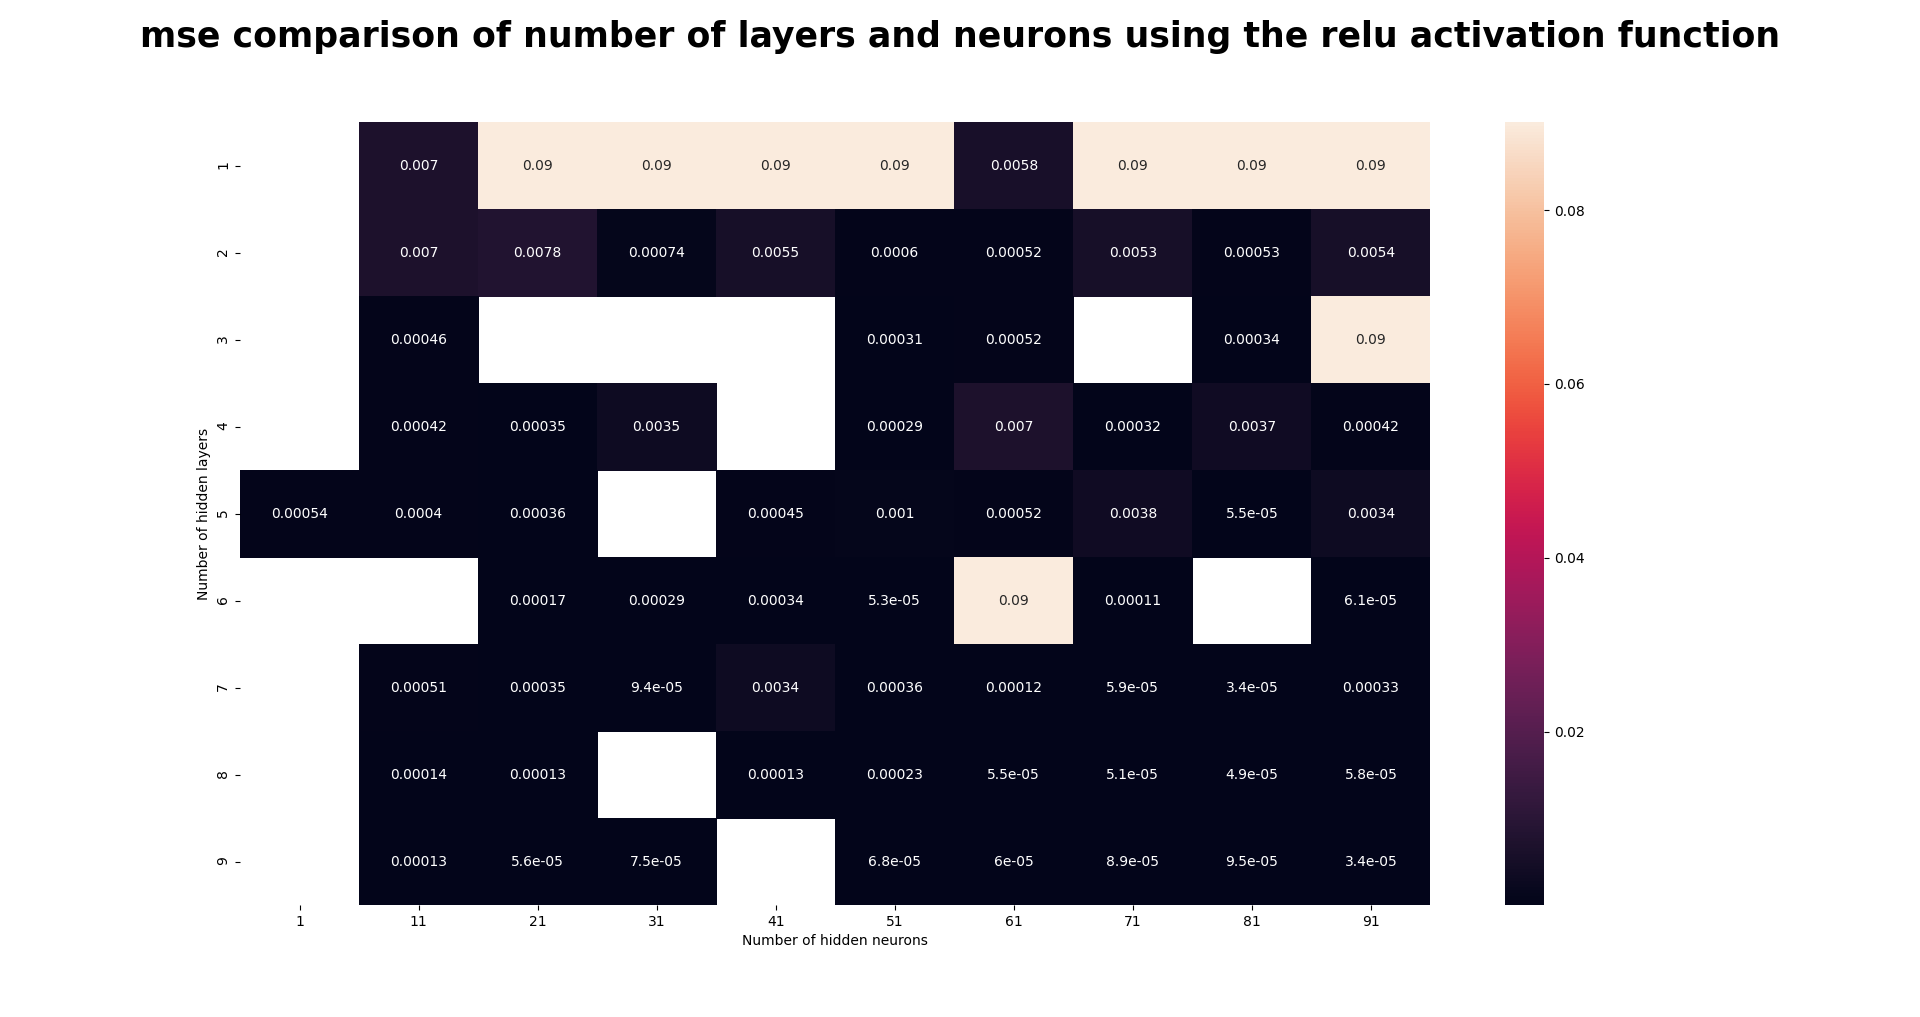
\includegraphics[width = 1\linewidth]{C:/Users/Sander/Documents/GitHub/FYS-STK4155/Project2/Project2/Report/Figures/heatmapOLS_TOTAL_reluMSE_REAL.PNG}
\caption{\label{fig:heatmap2} Heatmap for different number of hidden layers and neurons using the RELU activation function. This is the OLS equivalent.}
\end{figure}

\begin{figure}[H]
\centering
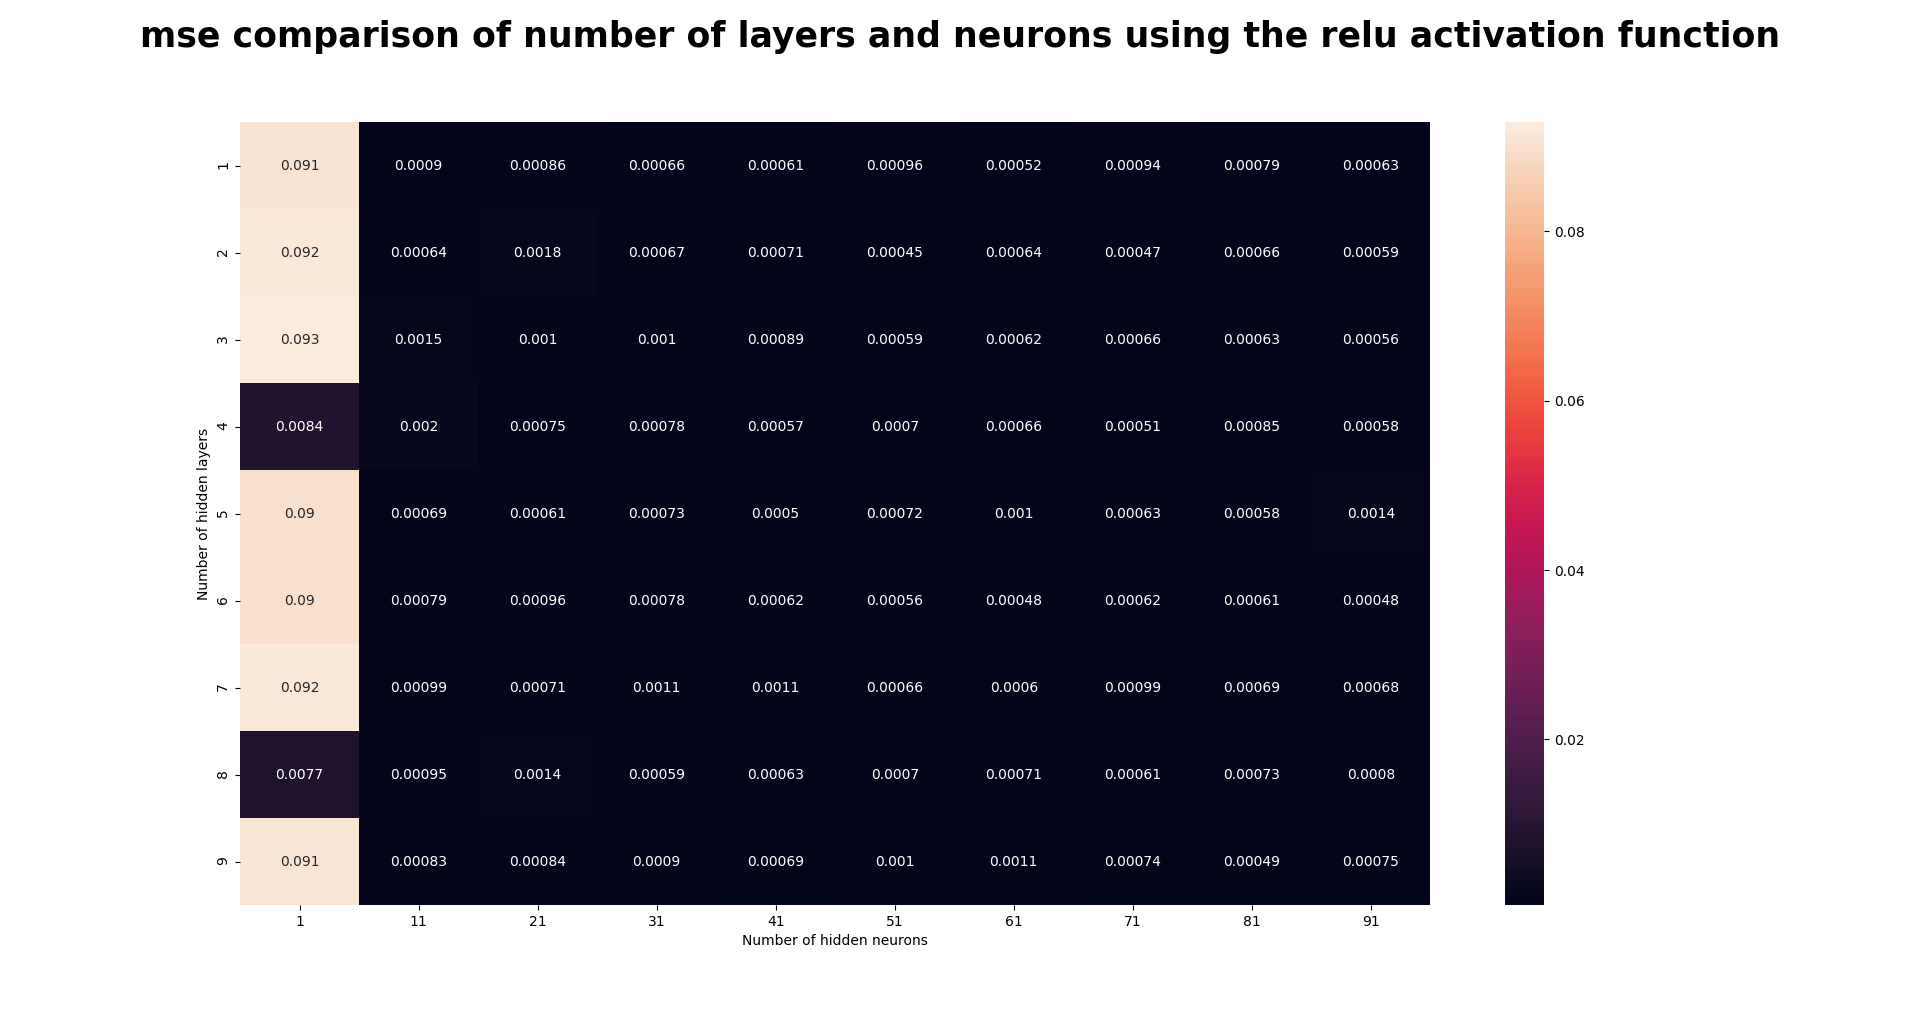
\includegraphics[width = 1\linewidth]{C:/Users/Sander/Documents/GitHub/FYS-STK4155/Project2/Project2/Report/Figures/heatmapOLS_TOTAL_reluMSE_sci_REAL.PNG}
\caption{\label{fig:heatmap3} Heatmap for different number of hidden layers and neurons using the RELU activation function with the Scikit implementation. This is the OLS equivalent.}
\end{figure}

\noindent One can observe from figure \ref{fig:heatmap2} that my own network experienced overflow at given layer/neuron configurations, as some of the squares in the heatmap is not included. This is particularly the case when there is only 1 hidden neuron in the layers. However, the network seems stable for a larger number of neurons in the layers. For hidden neurons above 30 and hidden layers above 5 it can be observed from figure \ref{fig:heatmap2} that the network is able to produce MSEs of under $0.0003$ which is lower than that of the sigmoid implementation. The Scikit implementation seems to be stable at any and all configurations of hidden layers and neurons. However, when there is only 1 neuron per hidden layer, the network gives a really high MSE. It is likely that the Scikit package includes some anti-overflow procedures that makes the algorithm able to deal with the overflow, but the neuron/layer configuration here still yields terrible results. We also observe that the MSE of the Scikit implementation is lower than that of my own implementation. These observations are compatable with those observed in figures \ref{fig:MSEvsLrateTOTAL1} to \ref{fig:MSEvsLrateTOTAL8}. 
\\
The leaky RELU implementation is plotted in figure \ref{fig:heatmap4}

\begin{figure}[H]
\centering
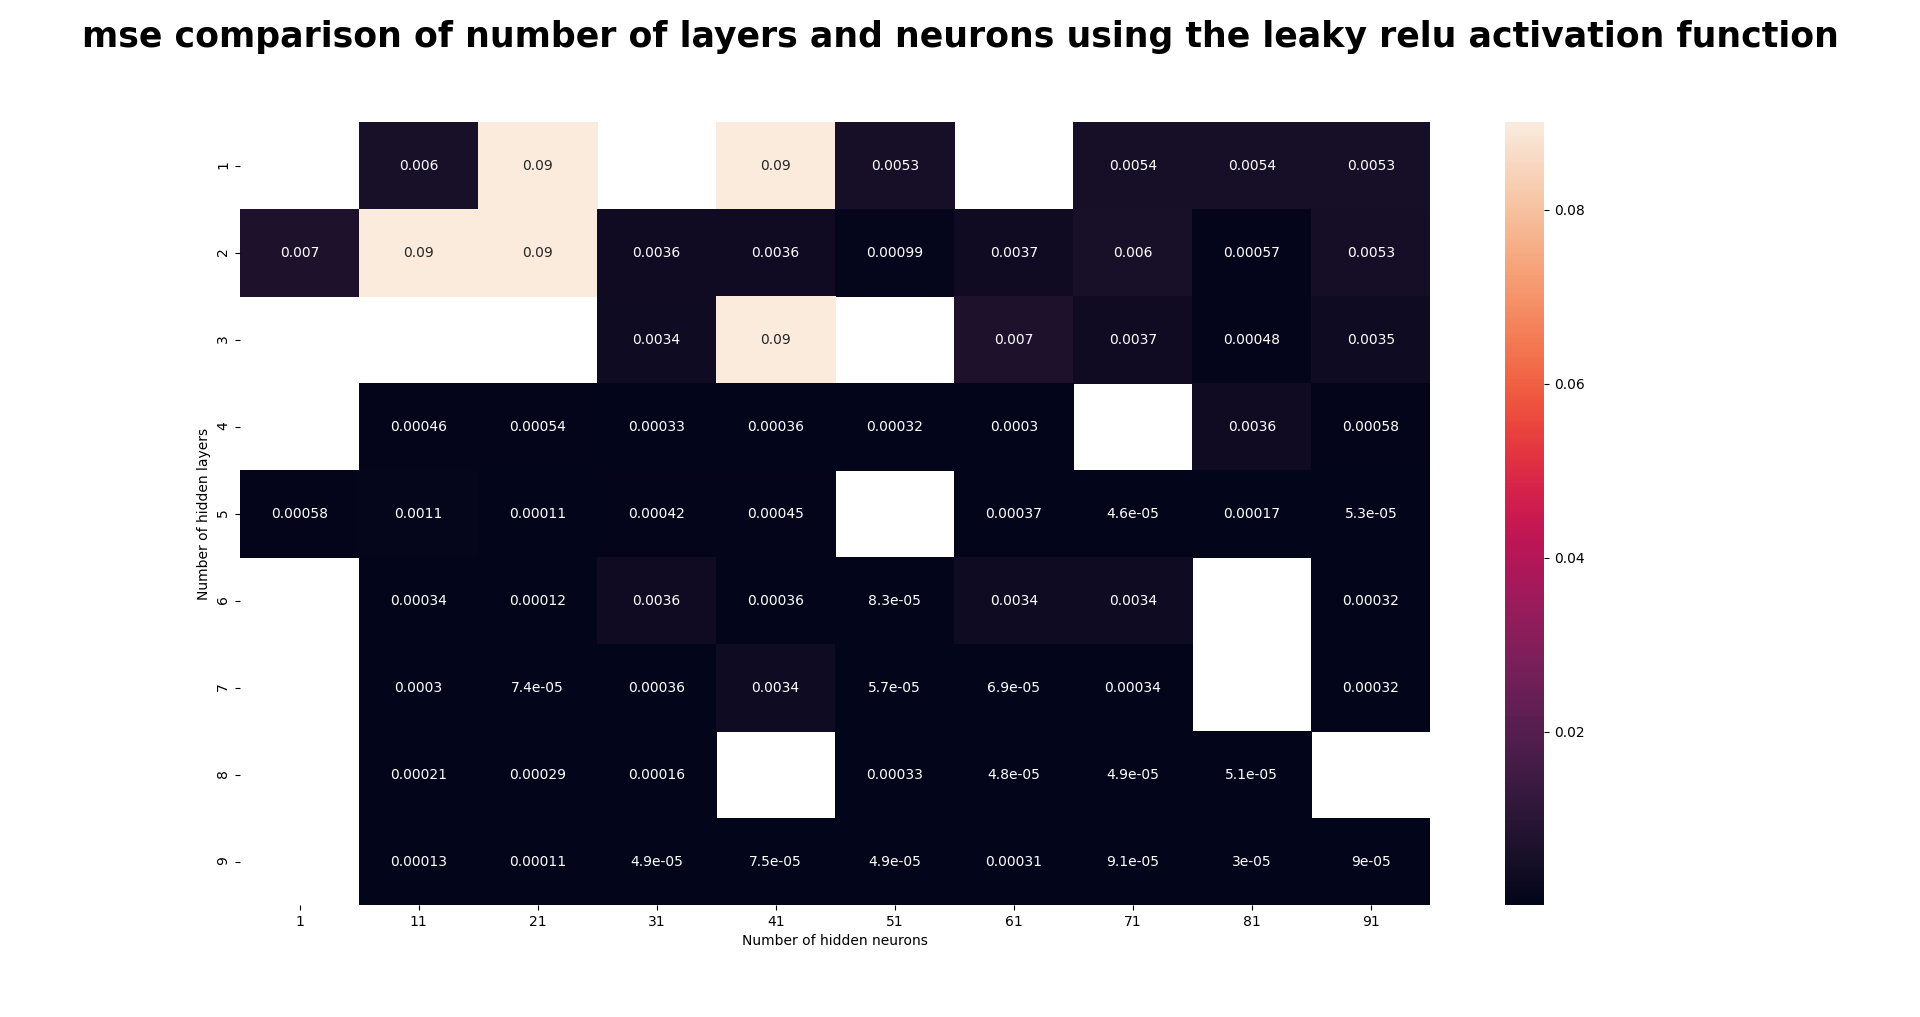
\includegraphics[width = 1\linewidth]{C:/Users/Sander/Documents/GitHub/FYS-STK4155/Project2/Project2/Report/Figures/heatmapOLS_TOTAL_leakyreluMSE_REAL.PNG}
\caption{\label{fig:heatmap4} Heatmap for different number of hidden layers and neurons using the leaky RELU activation function with the Scikit implementation. This is the OLS equivalent.}
\end{figure}

\noindent One can observe from figure \ref{fig:heatmap4} that it resembles my own RELU implementation seen in figure \ref{fig:heatmap2}. However, the algorithms is more unstable and there are many overflows occurring even for more layers and neurons. However, the MSE in the leaky RELU implementation seems to yield similar MSE values to the RELU implementation (slightly higher).

\begin{center}
\large{\textbf{Ridge equivalent implementation}}
\end{center}

\noindent We now aim to perform the above analysis, but using the Ridge equivalent implementation. The Ridge implementation works similar to that of linear regression, but we here add the penalty parameter while the neural network performs the back propagation. The weights are then adjusted with the penalty parameter in mind and the result is a reduction in what weights contribute to the overall output of the network. The penalty parameter was in this case set to $0.001$ as this was seen to yield good results in the previous project. 

MSE/r2 vs laernrates for ridge

\begin{figure}[H]
\centering
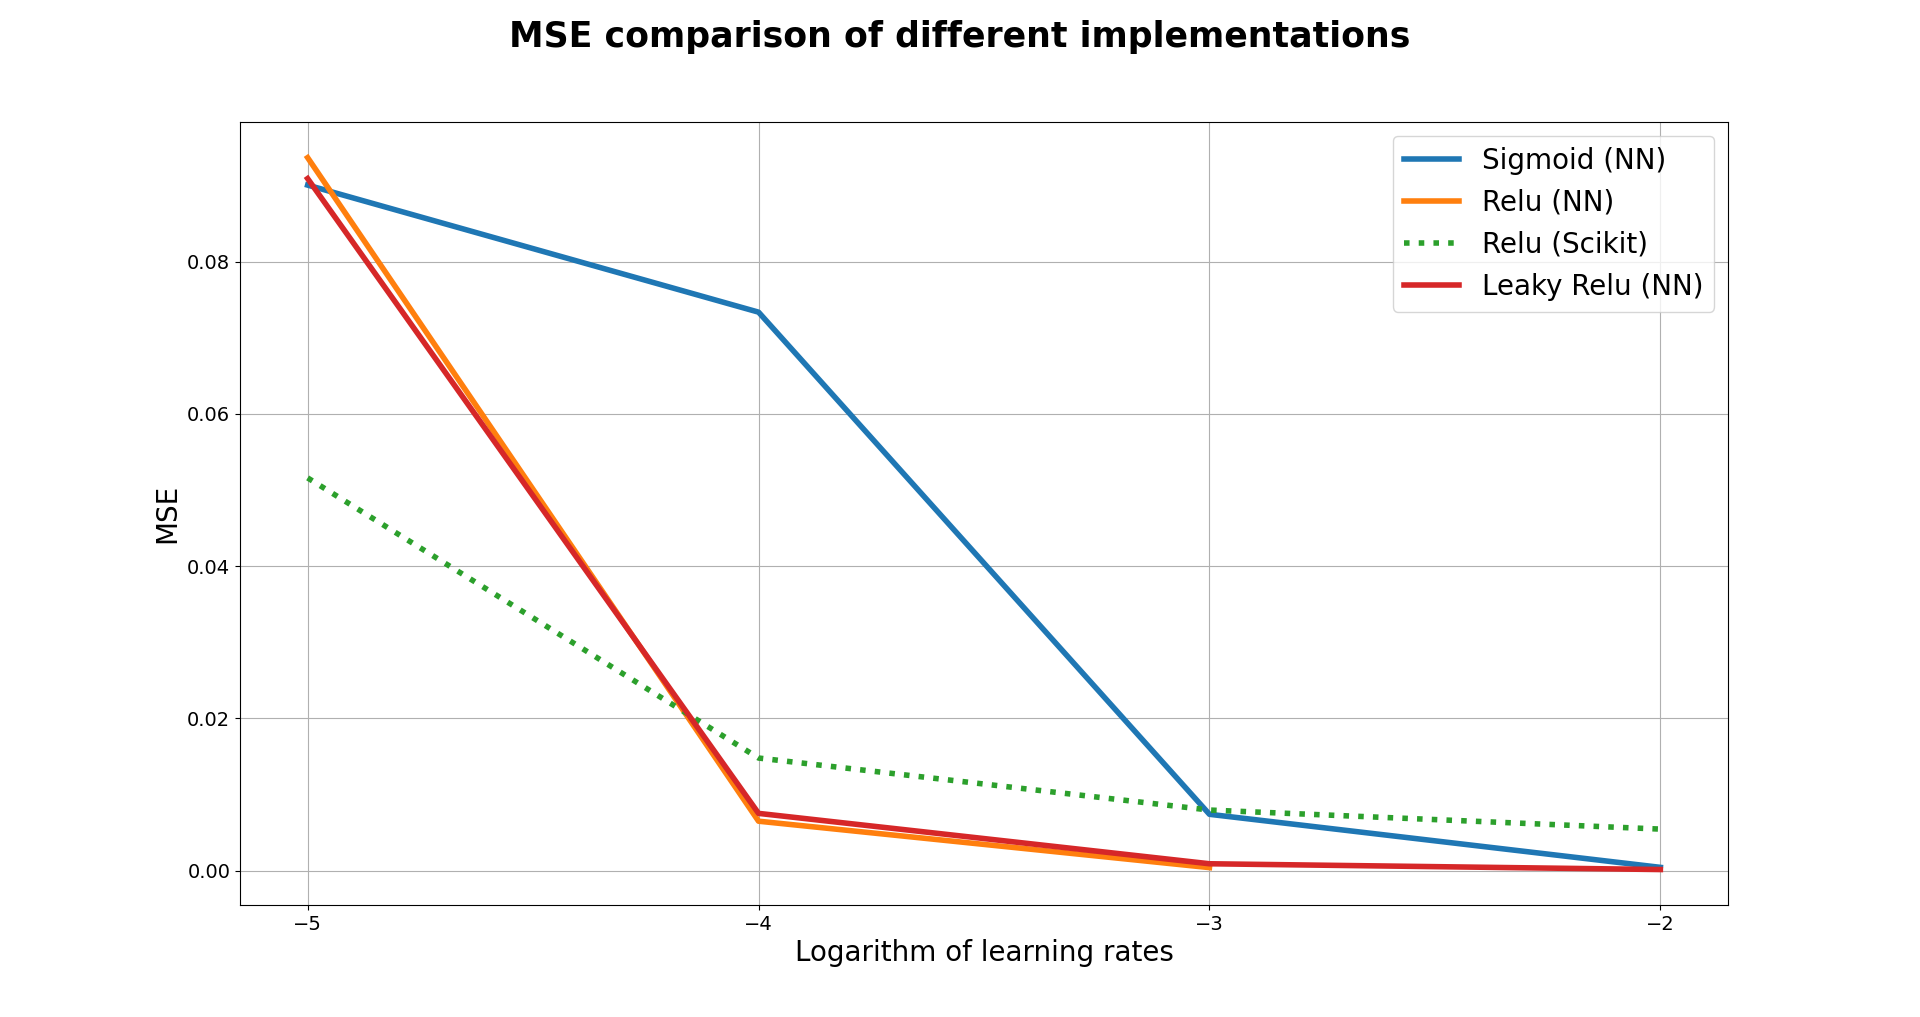
\includegraphics[width = 1\linewidth]{C:/Users/Sander/Documents/GitHub/FYS-STK4155/Project2/Project2/Report/Figures/MSEvsLearn_Ridge_TOTAL_epoch2000_batch2.PNG}
\caption{\label{fig:MSEvsLrateTOTAL8} The MSE as function of number of learning rate for the three activation functions when we utilize 2000 epoch iterations and a batch size of 2. This is the Ridge equivalent.}
\end{figure}

\begin{figure}[H]
\centering
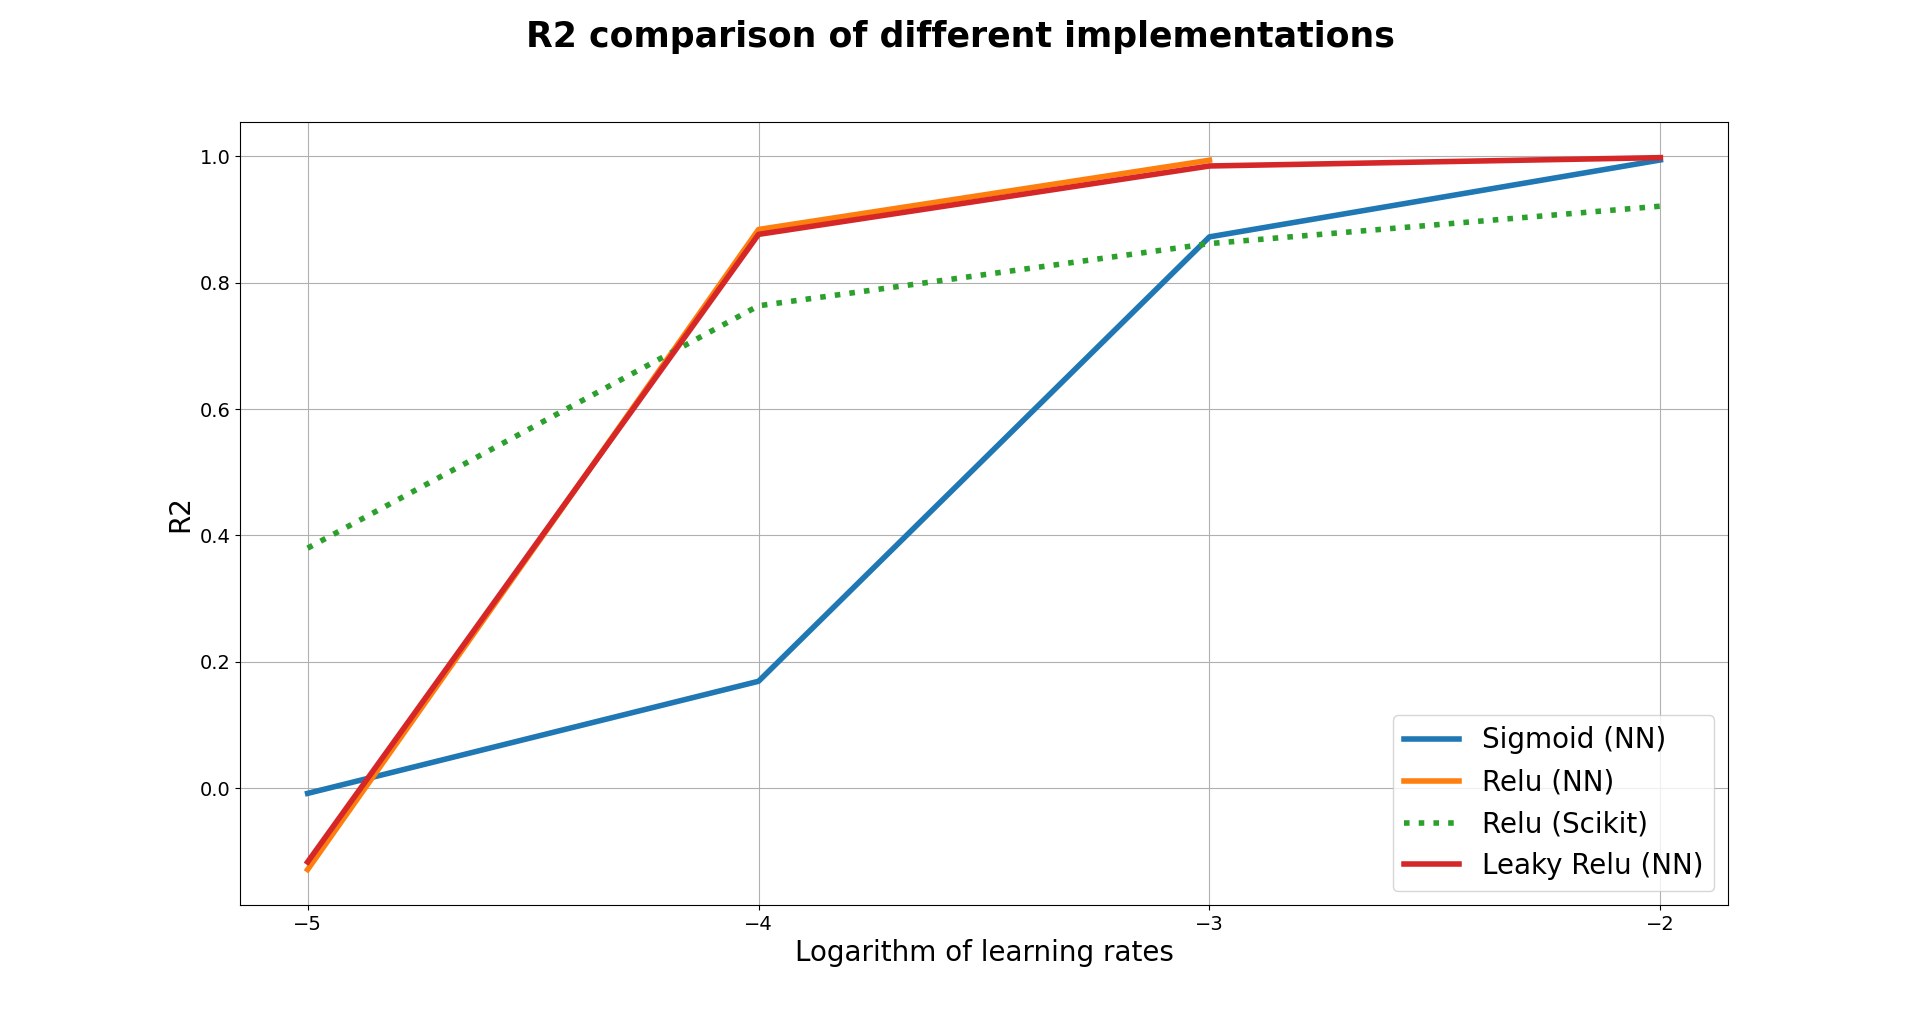
\includegraphics[width = 1\linewidth]{C:/Users/Sander/Documents/GitHub/FYS-STK4155/Project2/Project2/Report/Figures/MSEvsLearn_Ridge_TOTAL_epoch2000_batch2_r2.PNG}
\caption{\label{fig:MSEvsLrateTOTAL9} The $R^2$ as function of number of learning rate for the three activation functions when we utilize 2000 epoch iterations and a batch size of 2. This is the Ridge equivalent.}
\end{figure}

\begin{figure}[H]
\centering
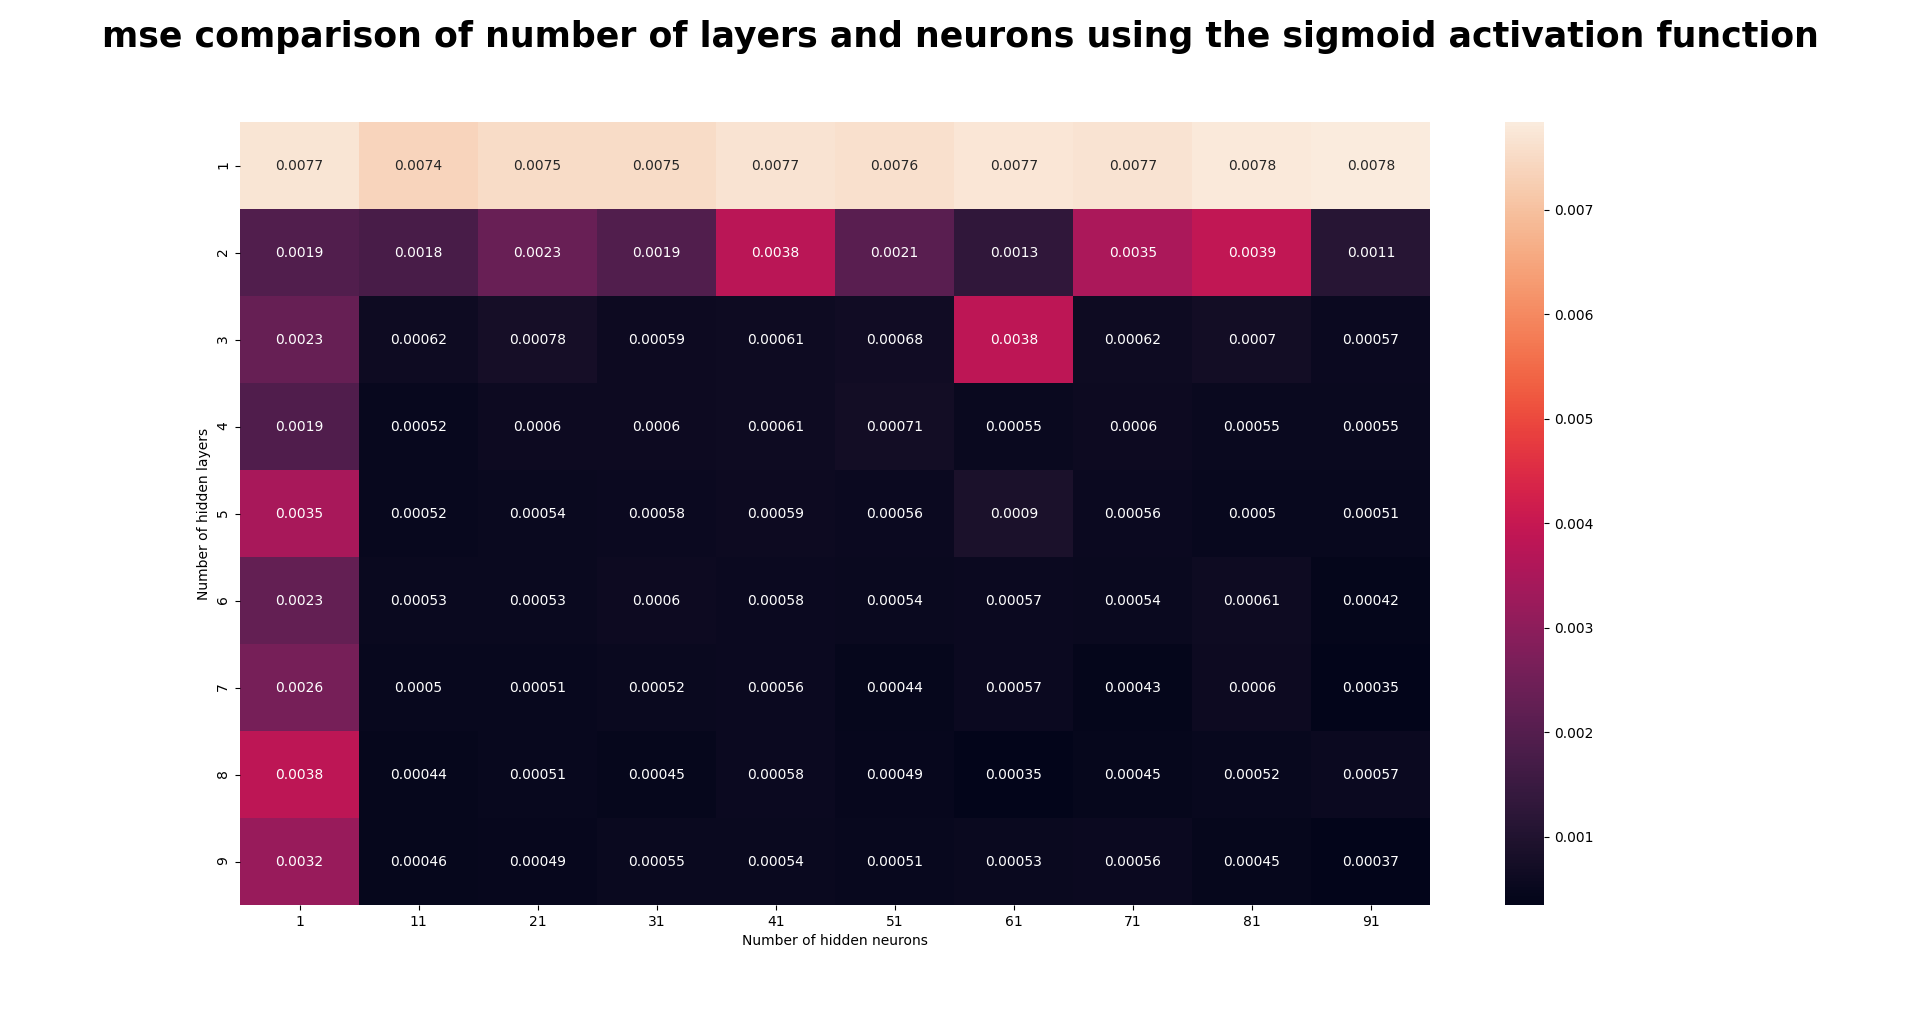
\includegraphics[width = 1\linewidth]{C:/Users/Sander/Documents/GitHub/FYS-STK4155/Project2/Project2/Report/Figures/heatmapRidge_TOTAL_sigmoid_REAL.PNG}
\caption{\label{fig:heatmap5} Heatmap for different number of hidden layers and neurons using the sigmoid activation function. This is the Ridge equivalent.}
\end{figure}

\begin{figure}[H]
\centering
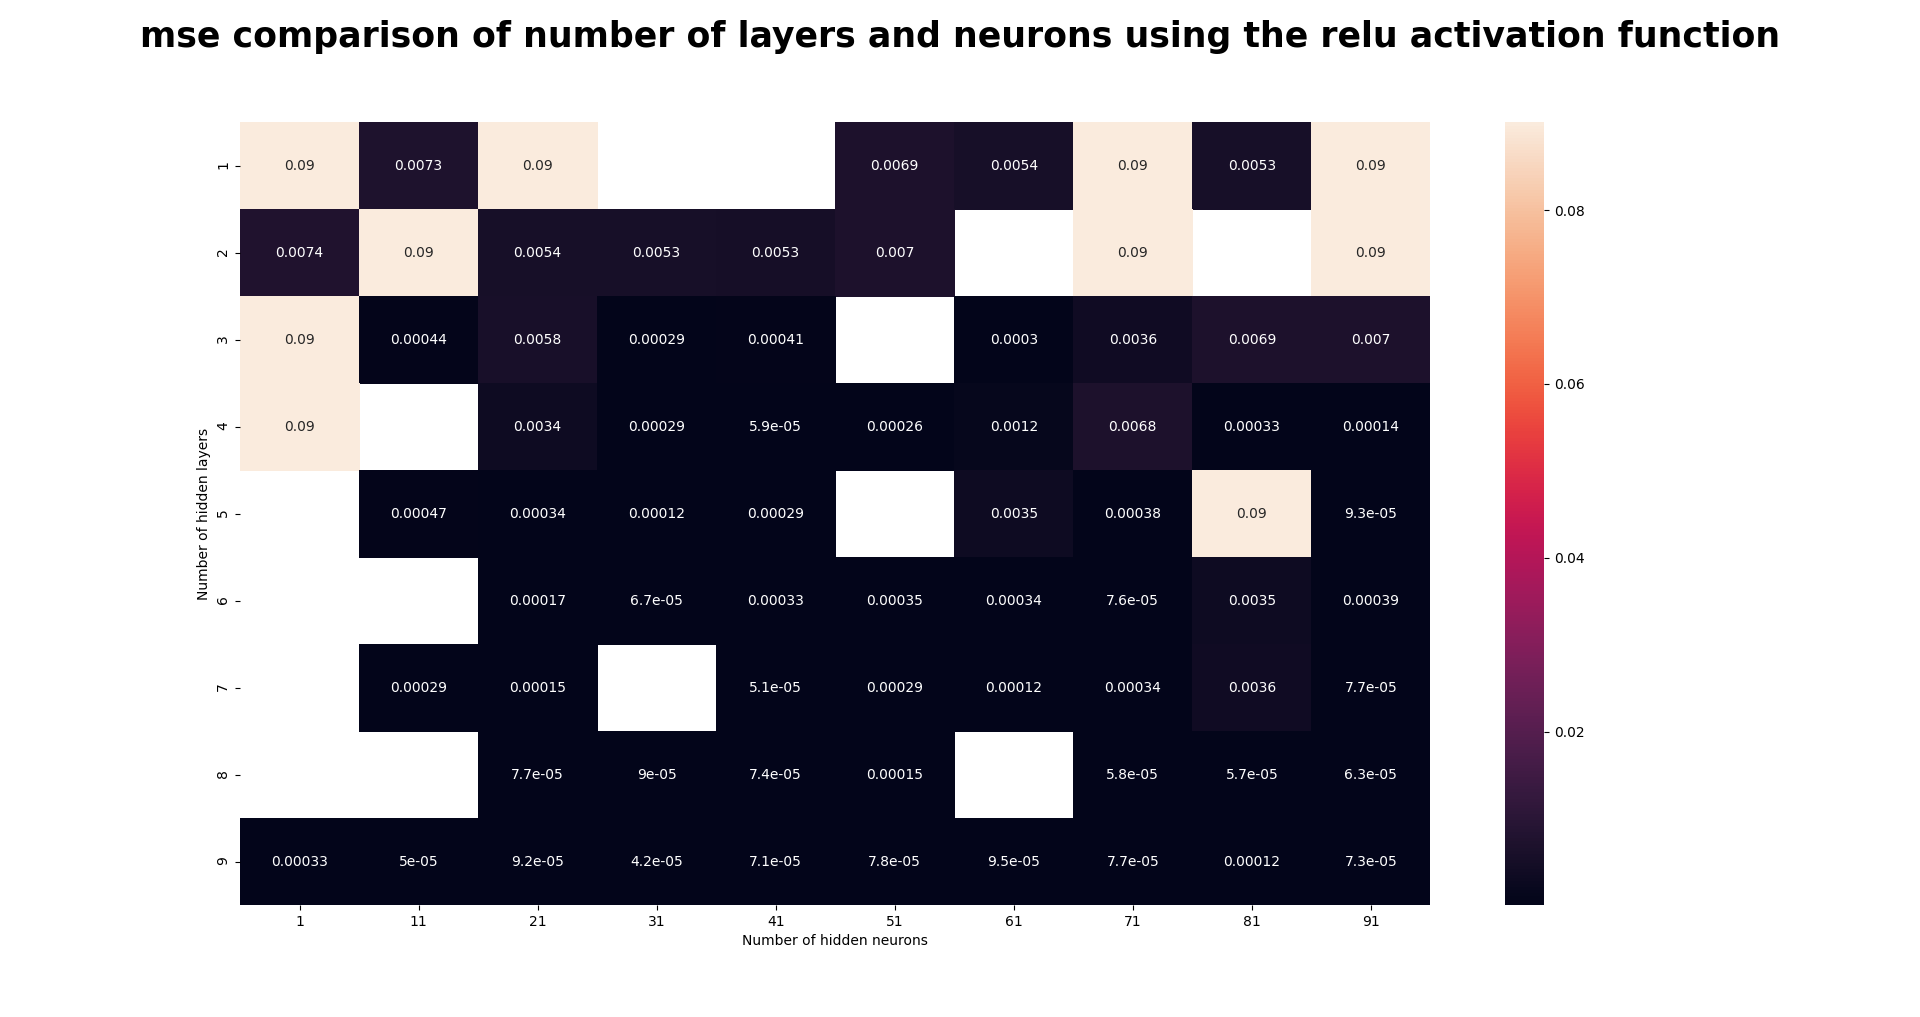
\includegraphics[width = 1\linewidth]{C:/Users/Sander/Documents/GitHub/FYS-STK4155/Project2/Project2/Report/Figures/heatmapRidge_TOTAL_relu_REAL.PNG}
\caption{\label{fig:heatmap6} Heatmap for different number of hidden layers and neurons using the sigmoid activation function. This is the Ridge equivalent.}
\end{figure}

\begin{figure}[H]
\centering
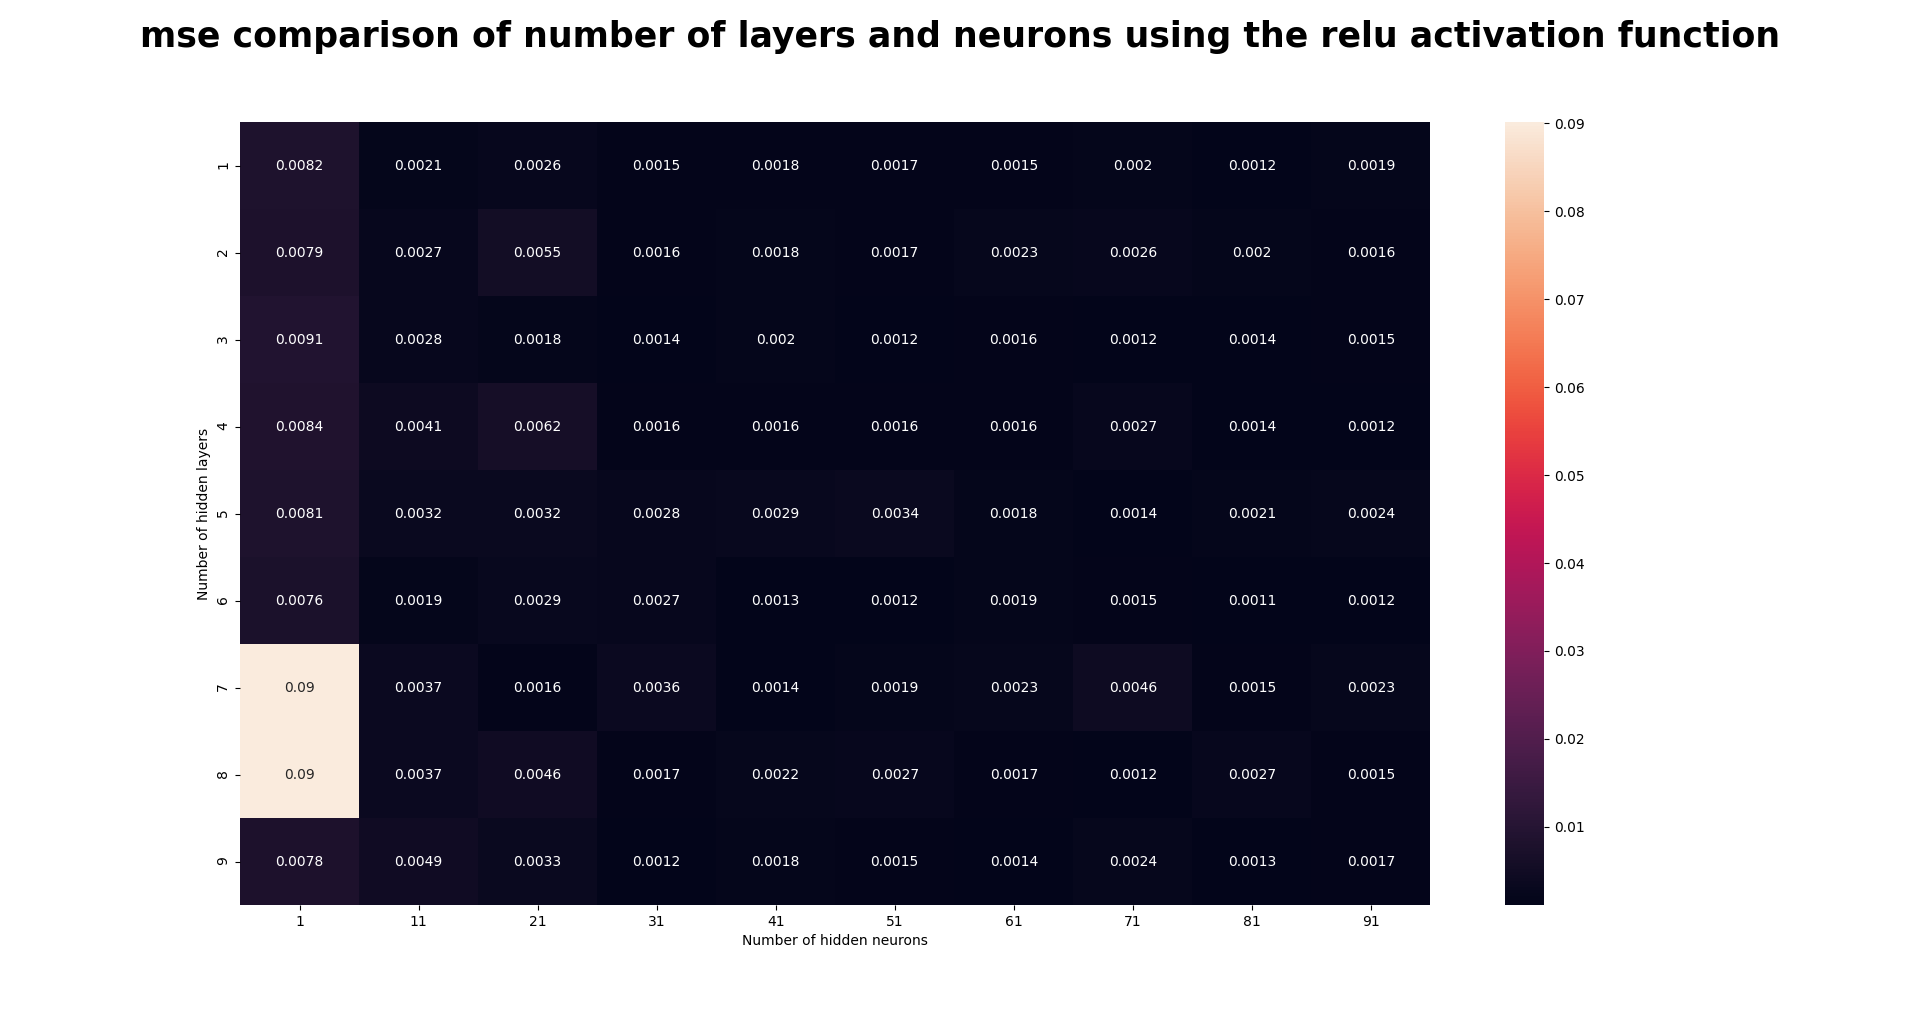
\includegraphics[width = 1\linewidth]{C:/Users/Sander/Documents/GitHub/FYS-STK4155/Project2/Project2/Report/Figures/heatmapRidge_TOTAL_relu_sci_REAL.PNG}
\caption{\label{fig:heatmap7} Heatmap for different number of hidden layers and neurons using the Scikit RELU activation function. This is the Ridge equivalent.}
\end{figure}

\begin{figure}[H]
\centering
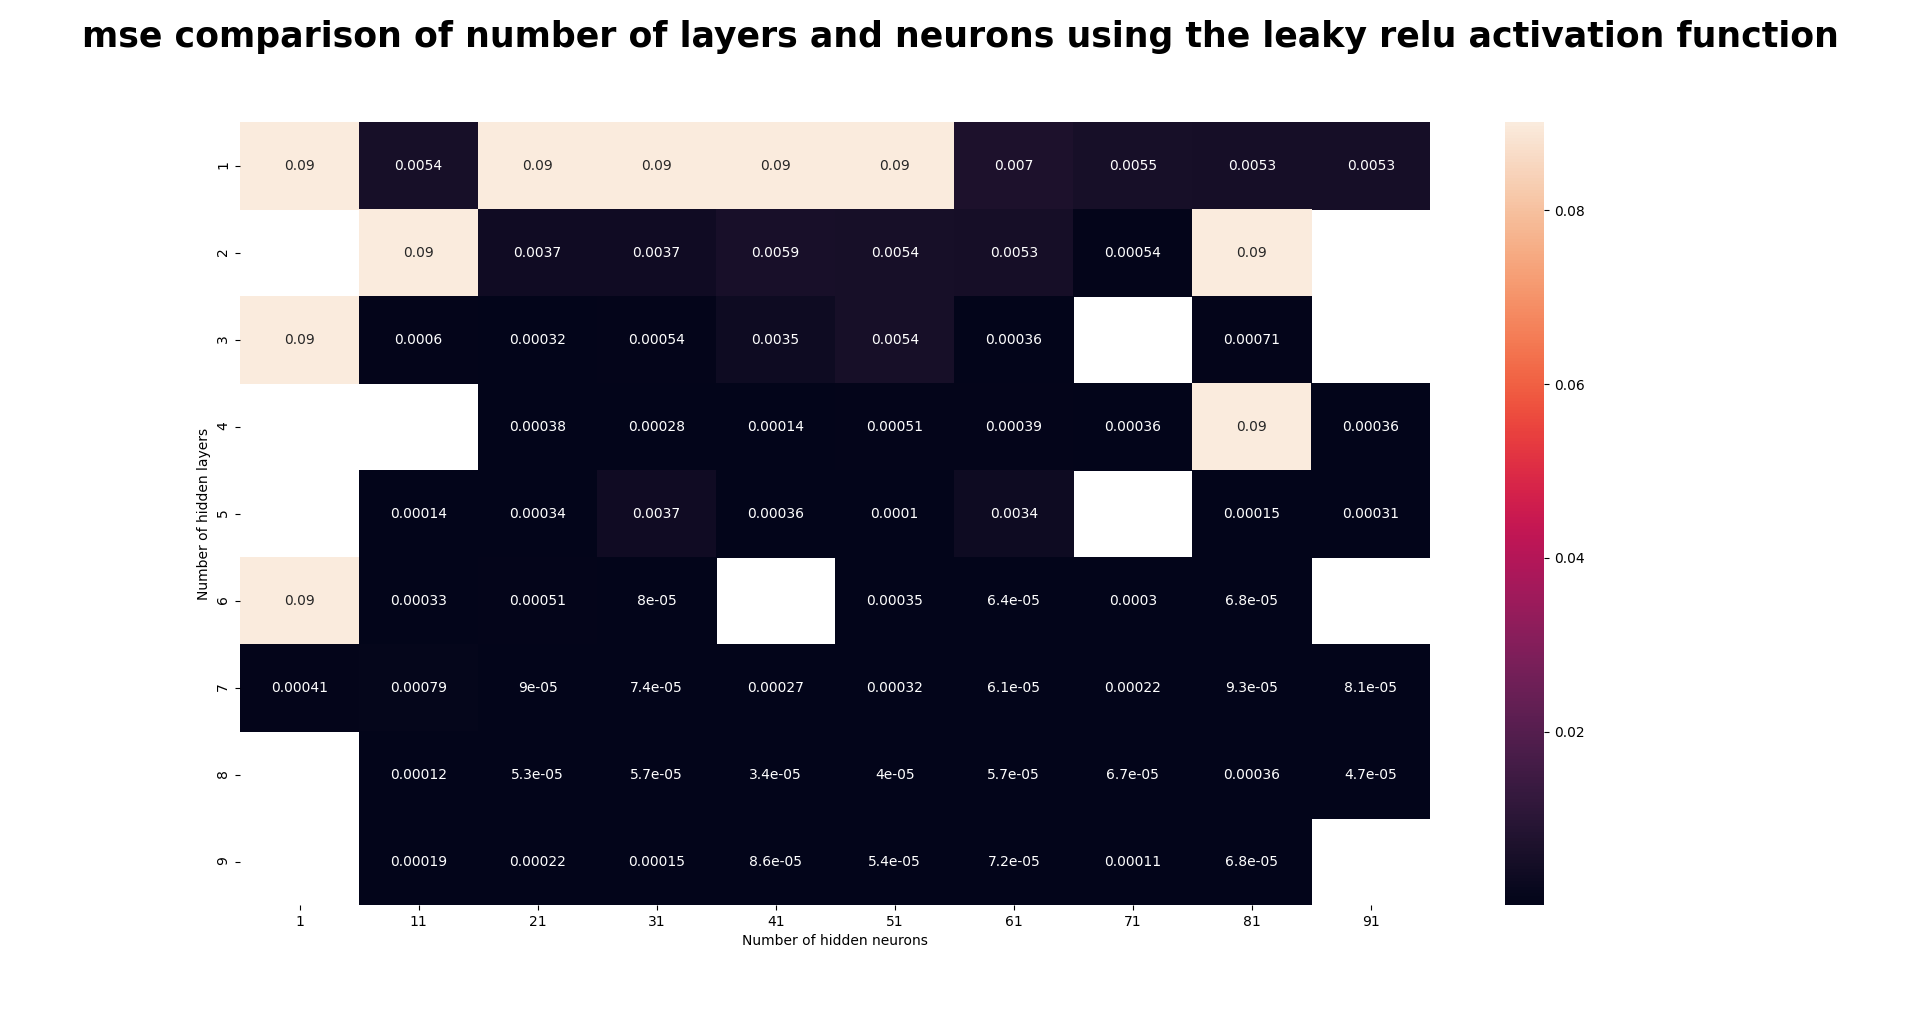
\includegraphics[width = 1\linewidth]{C:/Users/Sander/Documents/GitHub/FYS-STK4155/Project2/Project2/Report/Figures/heatmapRidge_TOTAL_leakyrelu_REAL.PNG}
\caption{\label{fig:heatmap8} Heatmap for different number of hidden layers and neurons using the leaky RELU activation function. This is the Ridge equivalent.}
\end{figure}

\newpage

\begin{center}
\Large{\textbf{Exercise d): Neural network classification}}
\end{center}

\begin{center}
\large{\textbf{Data set of hand-written digits}}
\end{center}

\noindent In this exercise we aim to classify hand-written digits given in the MNIST data set which can be downloaded from \href{{http://yann.lecun.com/exdb/mnist/}}{\nolinkurl{http://yann.lecun.com/exdb/mnist/}}. The data set contain both training data which will be used to train the neural network, and also test data which will be passed through the already trained network and compared to the actual answer. The data can be plotted and looks something like figure \ref{fig:DigitDataFig}

\begin{figure}[H]
\centering
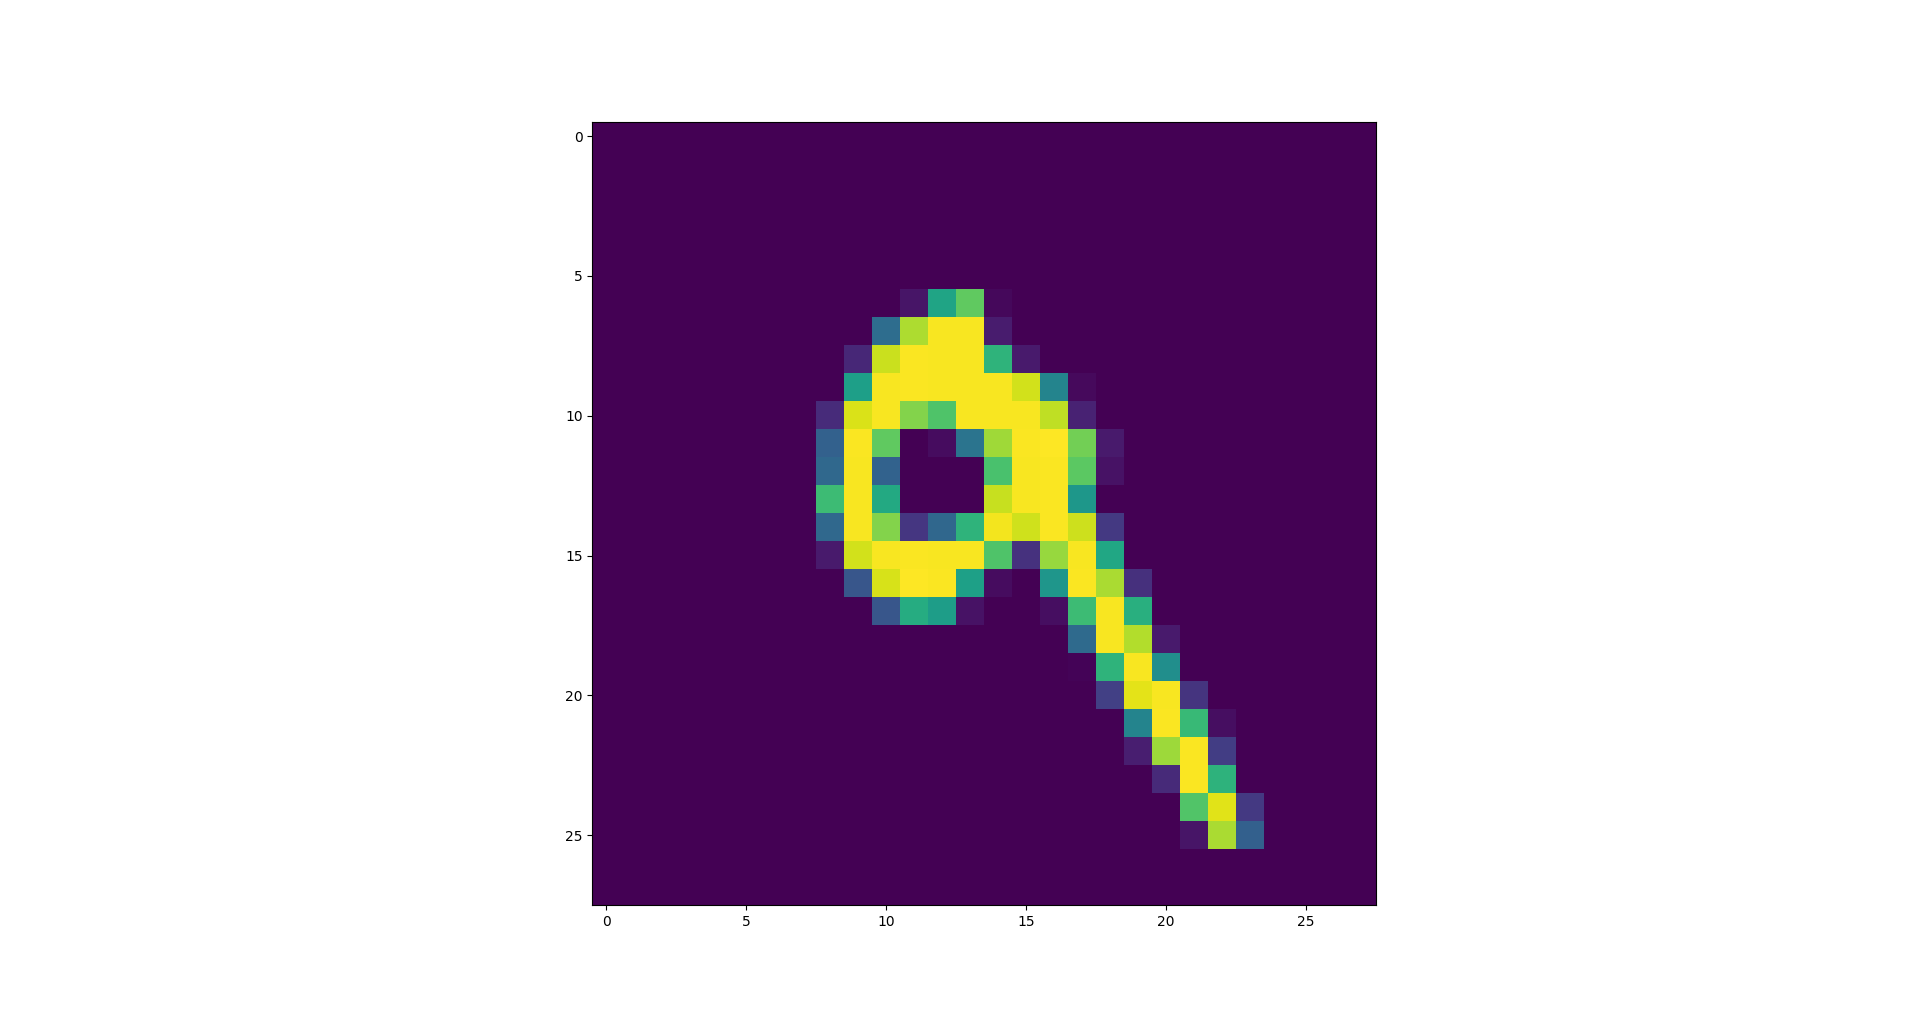
\includegraphics[width = 1\linewidth]{C:/Users/Sander/Documents/GitHub/FYS-STK4155/Project2/Project2/Report/Figures/DigitDataFig.PNG}
\caption{\label{fig:DigitDataFig} Example of how the training data looks. The digit shown is a hand-written digit that would be hard for a computer to recognize.}
\end{figure}

\begin{center}
\large{\textbf{Model evaluation principles}}
\end{center}

\noindent In order to evaluate a classification network we can no longer rely on the MSE or the $R^2$. Instead, we rely on using the accuracy score. The accuracy score is simply the correct number of prediction by the neural network divided by the total number of prediction (including wrong ones) and is defined by equation \ref{eq:acc}

\begin{equation}\label{eq:acc}
\begin{aligned}
\textrm{Accuracy} = \frac{\sum_{i = 1}^n I(f_i = y_i)}{n}
\end{aligned}
\end{equation}

\noindent where the numerator is the sum of correctly predicted digits and n is the total number of predictions. 

\begin{center}
\large{\textbf{The softmax activation function}}
\end{center}

\noindent The softmax function is a function that aims to take an input (what is passed through the neural network) and create a probability distribution of m different probabilities (m is 10 since we are working with the numbers from zero to nine). This function is given by equation \ref{eq:softmax}

\begin{equation}\label{eq:softmax}
\begin{aligned}
P(Y = y) = \frac{e^{\textbf{X}\beta}}{\sum_{i = 1}^m e^{\textbf{X}\beta}} 
\end{aligned}
\end{equation}

\noindent where \textbf{X} is the design matrix, $\beta$ is the regression coefficients matrix or weights in the neural network and P(Y = y) is the probability distribution of different possible outcomes from the neural network prediction. The softmax function allows us to categorize the input, digits in this case, into m different categories, 10 in this case, based on the probability estimated by the neural network. We can utilize the softmax function function as the output function in the output layer of the neural network, while the hidden layer activation functions can still be another function such as the sigmoid, RELU or leaky RELU. 

\newpage

\begin{center}
\Large{\textbf{Exercise 1e) a}}
\end{center}

\noindent a

\newpage

\begin{center}
\Large{\textbf{Exercise 1f) a}}
\end{center}

\noindent a

\newpage

\begin{center}
\Large{\textbf{Conclusion}}
\end{center}

\noindent a

\newpage

\begin{center}
\Large{\textbf{Future work}}
\end{center}

\noindent a

\newpage

\begin{center}
\Large{\textbf{References}}
\end{center}

\begin{itemize}
  \item a
\end{itemize}

\end{document}
